%===============================================================================

\chapter{Úvod}
\label{chap:intro}

Přestože počátky neuronových sítí sahají až do padesátých let 20. století, v~posledních několika letech se jim dostává velmi velké pozornosti.
Neuronové sítě jsou výpočetním modelem, který je používaný ve strojovém učení.
Základní myšlenkou neuronových sítí je propojení velkého množství malých jednotek do velké struktury.
Neuronové sítě jsou použitelné v~mnoha odvětvích výpočetních technologií, např. rozpoznávání hlasu, detekce objektů na obrázku či videu nebo klasifikace.

Jednou z~nevýhod neuronových sítí je jejich trénování, které může trvat velmi dlouhou dobu v~řádu dnů či týdnů.
Trénování hlubokých neuronových sítí je obvykle velmi výpočetně náročné.
Jedním ze způsobů jak snížit časovou náročnost výpočtu jakéhokoliv druhu je použití distribuovaného výpočtu.
Novým problémem při distribuovaném výpočtu je dodatečná komunikace mezi výpočetními jednotkami.
Neuronové sítě můžou obsahovat miliony parametrů, jejich přenosy tak mají nezanedbatelný vliv na délku výpočtu.

Cílem této práce je vytvořit způsob, jak ověřit výhodnost distribuovaného trénování pro zadanou neuronovou síť.
V~této práci provedu analýzu trénování sítě vzhledem k~délce natrénování jedné dávky a délce přenosu vah sítě.
Z~těchto dvou hodnot můžu vypočítat odhad délky celého trénování a zrychlení dosaženého pomocí distribuovaného výpočtu.

První kapitola se po myšlenkové stránce dá rozdělit na dvě části.
První tři sekce tvoří první část kapitoly, která se zabývá teoretickým popisem a složením neuronových sítí.
Zde se nacházejí definice základních pojmů z~oblasti neuronových sítí.
Na to navazují poslední čtyři sekce, které popisují konkrétní návrhy neuronových sítí.
Tyto sítě se nazývají VGG16E, GoogLeNet, SqueezeNet a Resnet34.

Velmi důležitou oblastí z~teorie neuronových sítí je jejich trénování, které popisuje druhá kapitola.
Začátek kapitoly slouží k~popisu samotných trénovacích algoritmů.
Druhá sekce pak popisuje výpočet gradientu, který se používá v~algoritmech na začátku kapitoly.
Konec této kapitoly je věnován algoritmům pro trénování na více výpočetních jednotkách.

Třetí kapitola popisuje nejdůležitější část této práce.
Tou jsou odhady doby paralelního trénování neuronových sítí podle použité techniky trénování. 
Paralelní trénování je buď synchronní nebo asynchronní, odhady dob trénování jsou ve dvou sekcích této kapitoly.
Výpočtu zrychlení trénování sítě je věnována poslední část této kapitoly.

Následující kapitola se zabývá implementačními prostředky, které jsem použil, abych ověřil nebo vyvrátil správnost výpočtů navržených v~předchozí kapitole.
Pro trénování jsem použil knihovnu Tensorflow, proto zde popisuji její základní principy.
Kapitola také obsahuje popis prostření, ve kterém jsem provedl experimenty.

V~následující kapitole jsem popsal provedené experimenty a jejich výsledky.
Popis samotných experimentů je pochopitelně první částí této kapitoly.
Následující tři sekce této kapitoly se věnují třem způsobům trénování, které jsem popsal v~předchozí sekci.
V~každé sekci je několik grafů, které zobrazují závislost zrychlení trénování na počtu pracovních jednotek pro danou neuronovou síť a způsob distribuovaného trénování.
Nové informace odvozené z~každého grafu jsem popsal a zhodnotil.

Poslední částí této práce je shrnutí výsledků a poznatků, které jsem zjistil při jejím vypracování. 
Tato kapitola také obsahuje návrh mechanizmu pro lepší rozdělení komunikace při trénování.

Tato práce navazuje na semestrální projekt.
Ze semestrálního projektu jsem převzal kapitolu o~neuronových sítích, popis sítě VGG16E a trénovací množiny Caltech256.
Text převzatý ze semestrálního projektu je v~kapitolách \ref{chap:nns}, \ref{chap:train} a \ref{chap:impl}.

%===============================================================================

\chapter{Neuronové sítě}
\label{chap:nns}

Práce se zabývá neuronovými sítěmi, proto je nutné vysvětlit principy, na kterých pracují.
K~tomu slouží tato kapitola.
První dvě sekce se zabývají dvěma nejrozšířenějšími typy neuronových sítí: dopřednými plně propojenými a konvolučními.
Třetí sekce je věnována těm částem neuronových sítí, které nepoužívají žádné neurony.
Poslední čtyři sekce popisují čtyři různé neuronové sítě, se kterými jsem experimentoval v~této práci.

Počátky neuronových sítí spadají až do roku 1957, kdy Frank Rosenblatt \cite{Rosenblatt1958} vytvořil první neuronovou síť -- perceptron.
Neuronové sítě jsou inspirovány neurony živých organizmů.
Historií a teorií se zabývají Ian Goodfellow, Yoshua Bengio a Aaron Courville v~knize Deep Learning \cite{Goodfellow-et-al-2016}.
Zpočátku měly neuronové sítě poměrně omezené možnosti.
To se změnilo v~90. letech, kdy počítače byly dostatečně výkonné na to, aby zvládly natrénovat několikavrstvé dopředné sítě pomocí algoritmu back-propagation.
Neuronové sítě se skládají z~malých jednotek, které se nazývají neurony.
Existuje několik způsobů, jak neurony propojit do struktury a vytvořit z~nich tak neuronovou síť.
Dva nejčastější způsoby jsou plně propojená síť a konvoluční neuronová síť, které jsou popsané v~následujících dvou podsekcích

\section{Dopředné neuronové sítě}
\label{sub:ffnn}

Dopředná neuronová síť je tvořena z~vrstev neuronů, které jsou na sebe napojeny -- výstup jedné vrstvy je napojen na vstup druhé vrstvy.
Pokud jsou propojeny všechny výstupy každé vrstvy na všechny vstupy následující vrstvy, pak se taková síť nazývá plně propojená.
Je to nejjednodušší architektura neuronové sítě.
První vrstva se nazývá vstupní a neprovádí žádný výpočet, pouze přeposílá vstup na následující vrstvu.
Poslední vrstva se nazývá výstupní.
Ostatní vrstvy se nazývají skryté vrstvy.
Diagram \ref{fig:ffcnn} ukazuje dopřednou neuronovou síť se čtyřmi neurony ve vstupní vrstvě, pěti neurony v~jedné skryté vrstvě a třemi neurony ve výstupní vrstvě.

\paragraph{Lineární jednotka.}
Lineární jednotka je typ neuronu, který provede sumu součinů vstupů neuronu a k~nim odpovídajících vah, a který k~této sumě přičte bias.
Činnost jednotky je popsaná následujícím způsobem \begin{equation}\sisetup{tight-spacing=true} \xi=W\cdot X+b,\label{eq:linear}\end{equation} kde $\xi$ je výstup, $W$ je vektor vah, $X$ je vstup a $b$ je bias.
Nevýhodou lineární jednotky je, že provádí pouze lineární transformace nad vstupem a pro popis složitějších funkcí musí být zkombinována s~nelineární aktivační funkcí.
Diagram \ref{fig:linear_unit} zobrazuje lineární jednotku s~aktivační funkcí $g()$.

\paragraph{Vrstva lineárních jednotek.}
Z~praktického hlediska je velkou výhodou lineární jednotky to, že je možné činnost jedné vrstvy plně propojené neuronové sítě definovat jako maticové násobení mezi vektorem vstupu a transponovanou maticí vah vrstvy.
První řádek matice vah vrstvy obsahuje váhy prvního neurony vrstvy atd..
Přičtení biasu odpovídá součtu výsledku maticového násobení a vektoru biasů.
Aktivační funkce je pak aplikována na každý prvek výsledku součtu.
Činnost takové vrstvy je popsaná jako \begin{equation}\sisetup{tight-spacing=true} \Xi=W^{T}\cdot X+B,\label{eq:linear_layer}\end{equation} kde $\Xi$ je výstup, $W$ je matice vah, $X$ je vstup a $B$ je bias.

\begin{figure}
\centering
\scalebox{0.8}{
\begin{tikzpicture}[auto,node distance=1em and 1em,>=triangle 45]
    \node [node_input](in1){$x_1$};
    \node [node_input,below=2em of in1](in2){$x_2$};
    \node [node_dot,below=1.5em of in2](in3){};
    \node [node_dot,below=0.2em of in3](in4){};
    \node [node_dot,below=0.2em of in4](in5){};
    \node [node_input,below=1.5em of in5](inn){$x_n$};
    \node [node_neuron,right=5em of in2](body){$\sum_{i=1}^{n}{W_{i}x_{i}}+b$};
    \node [node_neuron,right=5em of body](activ){$g()$};
    \node [node_point,right=3em of activ](out){};
    
    \draw[->] (in1) -- node{$W_1$} (body);
    \draw[->] (in2) -- node{$W_2$} (body);
    \draw[->] (inn) -- node{$W_n$} (body);
    \draw[->] (body) -- node{$\xi$} (activ);
    \draw[->] (activ) -- node{$y$} (out);
\end{tikzpicture}
}
\caption{Lineární jednotka včetně aktivační funkce $g()$.}
\label{fig:linear_unit}
\end{figure}

\subsection{Aktivační funkce}
\label{sub:activ}

Neuronová síť vytvořená kombinováním lineárních funkcí je také lineární funkce.
To znamená, že taková neuronová síť je nepoužitelná pro problémy, které nejsou lineárně separabilní.
Tento problém se řeší použitím nelineární aktivační funkce na výstup každého neuronu.
Jelikož taková síť obsahuje nelineární funkce, znamená to, že tato síť je také nelineární funkcí, a tudíž může být použita pro problémy, které jsou nelineárně separabilní.
Jako aktivační funkce se obvykle používají různé matematické funkce.

Nejoblíbenější funkcí je usměrněná lineární funkce (rectified linear unit, ReLU) popsaná následujícím způsobem \begin{equation}y=\left\{\begin{array}{ll}x&\mbox{pokud }x>0\\0&\mbox{pokud }x\leq 0\end{array}\right..\label{eq:relu}\end{equation}
Grafické znázornění této funkce je na obrázku \ref{gr:relu}.
Výhodou této funkce je její nízká výpočetní náročnost.
To platí i pro její derivaci.
Nevýhodou je, že neexistuje její derivace v~bodě 0, a že výstupní hodnoty pro $x>0$ nejsou nijak omezeny.

\begin{figure}
\centering
\begin{tikzpicture}
\begin{axis}
\addplot[color=black,domain=-4:4,xlabel={x},ylabel={y}]{max(0,x)};
\end{axis}
\end{tikzpicture}
\caption{Graf usměrněné lineární aktivační funkce.}
\label{gr:relu}
\end{figure}

Další oblíbenou aktivační funkcí je logistická funkce, která je definována následující rovnicí \begin{equation}y=\frac{1}{1+e_{-x}}.\label{eq:sigmoid}\end{equation}
Toto je jedna z~verzí logistické funkce, která se nazývá sigmoida.
Tato funkce je graficky znázorněna na obrázku \ref{gr:sigmoid}.
Výhodou této funkce je, že výstupní hodnoty jsou v~omezeném intervalu $y \in (-1,1)$, a že její derivace je definována ve všech bodech.
Nevýhodou je její výpočetní náročnost ve srovnání s~ReLU.

\begin{figure}
\centering
\begin{tikzpicture}
\begin{axis}
\addplot[color=black,domain=-4:4]{1/(1+exp(-x))};
\end{axis}
\end{tikzpicture}
\caption{Graf aktivační logistické funkce sigmoida.}
\label{gr:sigmoid}
\end{figure}

\begin{figure}
\centering
\scalebox{0.8}{
\begin{tikzpicture}[auto,node distance=1em and 1em,>=triangle 45]
    \node [node_input](in1){$x_1$};
    \node [node_input,below=3em of in1](in2){$x_2$};
    \node [node_input,below=4em of in2](in3){$x_3$};
    \node [node_input,below=3em of in3](in4){$x_4$};
    
    \node [node_neuron,right=7em of in1](h1){};
    \node [node_neuron,below=of h1](h2){};
    \node [node_neuron,below=of h2](h3){};
    \node [node_neuron,below=of h3](h4){};
    \node [node_neuron,below=of h4](h5){};
    
    \node [node_neuron,right=7em of h1](out1){};
    \node [node_neuron,right=7em of h3](out2){};
    \node [node_neuron,right=7em of h5](out3){};
    
    \node [node_point,right=3em of out1](y1){};
    \node [node_point,right=3em of out2](y2){$y_2$};
    \node [node_point,right=3em of out3](y3){$y_3$};
    
    \draw[->] (out1) -- node{$y_1$} (y1);
    \draw[->] (out2) -- node{$y_2$} (y2);
    \draw[->] (out3) -- node{$y_3$} (y3);
    
    \foreach \i in {1,...,4}
    {
        \foreach \j in {1,...,5}
        {
            \draw[->] (in\i) -- (h\j);
        }
    }
    
    \foreach \i in {1,...,5}
    {
        \foreach \j in {1,...,3}
        {
            \draw[->] (h\i) -- (out\j);
        }
    }
\end{tikzpicture}
}

\caption{
Dopředná plně propojená neuronová síť.
Pro zjednodušení diagramu nejsou zakresleny aktivační funkce neuronů.
}
\label{fig:ffcnn}
\end{figure}

\section{Konvoluční neuronové sítě}
\label{sub:cnn}

Konvoluční neuronové sítě (convolutional neural networks, CNN) jsou druhem neuronové sítě, ve které jsou neurony propojeny takovým způsobem, že jedna vrstva sítě počítá konvoluce mezi vstupem do vrstvy a váhami sítě.
První konvoluční neuronovou síť představil v~roce 1989 Yann LeCun \cite{LeCun1989}, který ji použil k~rozpoznávání číslic.
V~roce 2012 vyhrál Alexandr Krizhevsky soutěž ImageNet Large Scale Visual Recognition Challenge (ILSVRC) \cite{Krizhevsky2012} s~konvoluční neuronovou sítí, to pomohlo popularizaci tohoto druhu neuronové sítě.
Tato metoda byla výrazně úspěšnější než její konkurence.
Další výhodou konvolučních sítí je velká dostupnost datových sad a grafických karet, které dokážou zpracovat velké množství obrázků za sekundu.
Konvoluční neuronová síť se skládá ze dvou typů vrstev: konvoluční vrstvy a podvzorkovací vrstvy.

\subsection{Konvoluce}
\label{sub:conv_definition}

Konvoluce je matematická operace nad dvěma funkcemi s~argumentem z~oblasti reálných čísel, která se značí symbolem $*$.
Rovnice \begin{equation}s(t)=(x*w)(t)=\int x(a)w(t-a)da\label{eq:convolution}\end{equation} zobrazuje konvoluci nad dvěma funkcemi $x$ a $w$.
Jejím výsledkem je funkce $s$.

Problémem předchozí definice je to, že pracuje nad spojitými funkcemi.
Pro praktické použití je vhodnější konvoluce, která pracuje nad diskrétními funkcemi.
Ta je definována jako \begin{equation}s(t)=(x*w)(t)=\sum_{a=-\infty}^{\infty}{x(t-a)h(a)}.\label{eq:discrete_convolution}\end{equation}

V~konvolučních neuronových sítích se obvykle provádí konvoluce mezi dvěma několikarozměrnými poli dat.
Jedním z~těchto dvou polí je vstup do konvoluční vrstvy a druhým je část trénovatelných vah této vrstvy.
Těmto několikarozměrným polím se říká tenzory.
Jelikož oba tenzory musí být možné uložit, předpokládá se, že každá funkce se skládá z~konečného počtu nenulových bodů, které je možné si uložit, a že funkce je nulová ve všech ostatních bodech. 
V~praxi to znamená, že je možné možné implementovat konvoluci nad poli s~konečných počtem prvků.
Vzorec \begin{equation}S(i,j)=(I*K)(i,j)=\sum_{m}\sum_{n}{I(m,n)K(i-m,j-n)}\label{eq:2D_discrete_convolution}\end{equation} ukazuje diskrétní konvoluci nad dvěma dvourozměrnými poli $I$ a $K$.

\subsection{Konvoluční vrstva}
\label{sub:conv_layer}

Důležitou částí CNN jsou konvoluční vrstvy.
Každý neuron této vrstvy je propojený pouze s~několika neurony předchozí vrstvy nebo s~body vstupního obrazu, pokud je tato vrstva první.
Tyto vstupní neurony nebo body tvoří okolí jednoho neuronu nebo bodu.
Neurony konvoluční vrstvy jsou organizovány do rovin.
Všechny roviny jsou tvořeny stejným počtem neuronů.
Všechny neurony ve stejné rovině mají stejnou množinu vah.
To je založeno na úvaze, že všechny neurony v~rovině slouží k~detekci stejného příznaku.
Každý neuron provádí skalární součin mezi jeho vstupem a množinou vah roviny, ve které se nachází, je to tedy lineární jednotka.
Výstup všech neuronů v~jedné rovině se nazývá mapa příznaků.
Jedna rovina neuronů tak vlastně provede konvoluci mezi vstupem konvoluční vrstvy a množinou vah jejích neuronů.
Výstupy všech rovin neuronů tvoří výstup konvoluční vrstvy, který se označuje jako mapy příznaků.
Jeden neuron konvoluční vrstvy zobrazuje diagram \ref{fig:conv_neuron}.

Neurony konvoluční vrstvy slouží k~detekci příznaků (hrany, rohy, změna barvy atd.), které jsou pak uloženy v~mapách příznaků.
Následující vrstvy pak kombinují jednotlivé příznaky z~několika map na nové příznaky o~vyšší úrovni.

\begin{figure}
\centering
\scalebox{0.8}{
\begin{tikzpicture}[auto,x=1em,y=1em,z=1em,node distance=1em and 1em,>=triangle 45]
    \draw[fill=lightgray] (1.5,4.5) rectangle (10.5,10.5);
    \draw[fill=lightgray,xslant=1] (-9,10.5) rectangle (0,13.5);
    \draw[fill=lightgray,yslant=1] (10.5,-6) rectangle (13.5,0);
    
    \draw[step=3,xshift=1.5em,yshift=1.5em] (0,3) grid (9,9);
    \draw[xstep=3,ystep=1.5,xslant=1] (-9,10.5) grid (0,13.5);
    
    \draw[step=3] (0,0) grid (9,15);
    \draw[xstep=3,ystep=1.5,xslant=1] (-15,15) grid (-6,22.5);
    \draw[xstep=1.5,ystep=3,yslant=1] (9,-9) grid (16.5,6);
    
    \begin{scope}[shift={(20,0)}]
        \draw[fill=lightgray] (1.5,4.5) rectangle (10.5,10.5);
        \draw[fill=lightgray,xslant=1] (-9,10.5) rectangle (0,13.5);
        \draw[fill=lightgray,yslant=1] (10.5,-6) rectangle (13.5,0);
        
        \draw[step=3,xshift=1.5em,yshift=1.5em] (0,3) grid (9,9);
        \draw[xstep=3,ystep=1.5,xslant=1] (-9,10.5) grid (0,13.5);
        \draw[xstep=1.5,ystep=3,yslant=1] (10.5,-6) grid (13.5,0);
        
        \draw[dashed,gray] (1.5,4.5) -- (-9.5,4.5);
        \draw[dashed,gray] (1.5,10.5) -- (-9.5,10.5);
        \draw[dashed,gray] (4.5,13.5) -- (-6.5,13.5);
        \draw[dashed,gray] (1.5,7.5) -- (-6.5,7.5);
    \end{scope}
    
    \begin{scope}[shift={(40,9)}]
        \node [node_neuron](n){$\sum$};
        \node [node_neuron,right=2em of n](a){$g()$};
        \node [node_point,right=2em of a](o){};
        
        \draw[dashed,gray,->] (n) -- (a);
        \draw[dashed,gray,->] (a) -- (o);
        \draw[dashed,gray,->] (-9.5,1.5) -- (n);
        \draw[dashed,gray,->] (-9.5,-4.5) -- (n);
        \draw[dashed,gray,->] (-6.5,4.5) -- (n);
        \draw[dashed,gray,->] (-6.5,-1.5) -- (n);
    \end{scope}
\end{tikzpicture}
}
\caption{
Jeden neuron konvoluční vrstvy.
V~levé části diagramu je umístěn vstup do konvoluční vrstvy, které je tento neuron součástí.
Šedou barvou je zvýrazněna ta část vstupu, se kterou je neuron propojený.
Střední část diagramu obsahuje třírozměrný tensor sdílených vah neuronu/roviny.
V~pravé části je zobrazeno tělo neuronu označené symbolem $\sum$ a aktivační funkce $g()$.
}
\label{fig:conv_neuron}
\end{figure}

\section{Vrstvy neobsahující neurony}
\label{sec:noneuron}

Důležitou částí neuronových sítí jsou i vrstvy, které nepoužívají vůbec žádné neurony.
Tyto vrstvy slouží k~úpravě dat, které si mezi sebou předávají dvě jiné vrstvy.

\subsection{Vrstva maxpooling}
\label{sub:maxpooling}

Podvzorkování slouží ke snížení velikosti map příznaků, se kterými se v~konvolučních neuronových sítích pracuje.
Jednou z~myšlenek za podvzorkováním je to, že není důležitá přesná poloha příznaku, ale že stačí pouze jeho přibližná poloha vzhledem k~ostatním příznakům.
Druhou myšlenkou je snížení časové a paměťové náročnosti sítě.
To je důležité, protože v~sítích dochází ke zvyšování počtu map příznaků.
Snížení jejich velikosti by tak mělo omezit narůstání výpočetní složitosti v~pozdějších částech sítě.
Další výhodou podvzorkování je kontrola přetrénování.

Maxpooling je jedna z~možností jak provést podvzorkování.
Princip této vrstvy spočívá v~tom, že se čtvercové okolí bodu nahradí největší hodnotou z~tohoto okolí (včetně bodu samotného).
Krok maxpoolingu říká o~kolik bodů se musí posunout okolí pro získání dalšího bodu výsledku.
Pokud je krok roven jedné, velikost výstupu se rovná velikosti vstupu.
Vyšší velikost kroku způsobí snížení velikosti výstupu.

\begin{figure}
\centering
\scalebox{0.8}{
\begin{tikzpicture}[auto,x=1em,y=1em,z=1em,>=triangle 45]
    \draw[fill=lightgray] (3,3) rectangle (12,12);
    \draw[fill=lightgray] (33,6) rectangle (36,9);
    \draw[step=3,name=pre] (0,0) grid (18,18);
    \draw[step=3,name=post] (30,3) grid (39,12);
    
    \draw[gray,->] (18,18) -- (30,12);
    \draw[gray,->] (18,0) -- (30,3);
    
    \matrix[matrix of nodes,ampersand replacement=\&,inner sep=0,text height=3em,text width=3em,nodes={rectangle,anchor=center,minimum height=3em,minimum width=3em}]at(10em,10em){
    1 \& 5 \& 1 \& 2 \& 5 \& 4\\
    2 \& 4 \& 9 \& 1 \& 4 \& 6\\
    4 \& 6 \& 7 \& 8 \& 3 \& 7\\
    7 \& 4 \& 4 \& 3 \& 3 \& 9\\
    2 \& 4 \& 6 \& 7 \& 4 \& 1\\
    6 \& 8 \& 5 \& 2 \& 5 \& 6\\
    };
    
    \matrix[matrix of nodes,ampersand replacement=\&,inner sep=0,text height=3em,text width=3em,nodes={rectangle,anchor=center,minimum height=3em,minimum width=3em}]at(35.5em,8.5em){
    6 \& 9 \& 8\\
    7 \& 8 \& 9\\
    8 \& 8 \& 7\\
    };
\end{tikzpicture}
}
\caption{
Ukázka činnosti vrstvy maxpooling používající okolí bodu o~velikosti $3{\times}3$ a s~krokem 2.
Mapa příznaků nalevo je vstup do vrstvy a vpravo je výstup z~vrstvy.
Šedě je vyznačeno okolí jednoho bodu a k~němu odpovídající maximum.
}
\label{fig:maxpool}
\end{figure}

\subsection{Vrstva avgpooling}
\label{sub:avgpooling}

Tato vrstva byla navržena týmem z~univerzity Singapuru v~práci \cite{Lin2013}.
Konvoluční neuronové sítě jsou často ukončeny vektorizací map příznaků, plně propojenou vrstvou a vrstvou softmax.
Tento styl architektury je spojením konvoluční a plně propojené neuronové sítě.
Konvoluční část sítě tak slouží k~extrakci rysů a klasifikace se pak provádí pomocí plně propojené vrstvy.
Plně propojené vrstvy jsou ale náchylné k~přetrénování.

Jedním způsobem jak tento problém vyřešit je vrstva avgpooling.
Předpokládá se, že výstup poslední konvoluční vrstvy má stejný počet map příznaků jako je tříd na výstupu sítě.
Následující vrstva avgpool vypočítá průměry všech map příznaků a jejím výstupem tak bude vektor, který má délku rovnající se počtu tříd.
Síť bude ukončena vrstvou typu softmax.
Tento přístup vynucuje korespondenci mezi mapami příznaků a třídami a používá pouze nástrojů konvolučních neuronových vrstev.
Druhou výhodou je, že vrstva avgpool neobsahuje žádné parametry na rozdíl od plně propojené vrstvy.
Tím se odstraní nebezpečí přetrénování této vrstvy a zároveň se snižuje počet parametrů celé sítě, které je nutné přenést během paralelního trénování.

\subsection{Normalizace lokální odezvy}
\label{sub:lrn}

Součástí konvolučních neuronových sítí jsou také normalizační vrstvy, které slouží k~úpravě map příznaků, tak aby se ostatním vrstvám s~nimi lépe pracovalo.
To znamená, že jsou z~pohledu paralelního trénování velmi užitečné, protože obvykle neobsahují váhy, které je nutné přenášet.

Normalizace lokální odezvy (Local Response Normalization, LRN) byla vytvořena týmem z~univerzity v~Torontu a definována v~práci \cite{Krizhevsky2012}.
Inspirací bylo chování biologických neuronů, kde excitace jednoho neuronu snižuje aktivitu okolních neuronů.
Cílem této normalizace je podpoření soupeření neuronů na stejných souřadnicích v~sousedících rovinách ve stejné vrstvě sítě.
Rovnice \begin{equation}b^{i}_{x,y}=a^{i}_{x,y}/\left(k+{\alpha}\sum^{min(N-1,i+n/2)}_{j=max(0,i-n/2)}({a^{j}_{x,y}}^{2})\right)^{\beta}\label{eq:lrn}\end{equation} udává, jak vypočítat normalizaci pro každý výstup konvoluční vrstvy, kde $a^{i}_{x,y}$ je výstup neuronu $i$té roviny na souřadnicích $(x,y)$ a $b^{i}_{x,y}$ je jemu odpovídající výstup z~LRN.
$N$ je celkový počet rovin vrstvy, $n$ je počet sousedních vrstev, které mají vliv na výstup LRN a $\alpha$, $\beta$ a $k$ jsou hyperparametry.

\subsection{Normalizace dávek}
\label{sub:bn}

Normalizaci dávek (Batch Normalization, BN) navrhli Sergey Ioffe a Christian Szegedy v~práci \cite{Ioffe2015}.
Problémem při trénování sítě jsou změny rozložení aktivací neuronů.
Toto se obvykle řeší pomocí malého koeficientu učení a velkého počtu kroků trénování.
Normalizace dávek omezuje vliv tohoto jevu a umožňuje použít vyšší koeficient učení, který zrychlí trénování.
Tato normalizace se provádí pomocí statistických dat jedné dávky při trénování.
Vstupem do normalizace je dávka $\mathcal{B}=\{x_{1}, ...,x_{m}\}$ a výstupem je normalizovaná dávka $\mathcal{B}_{BN}=\{y_{i}=BN_{\gamma,\beta}(x_{i})\}$.
Rovnice \ref{eq:bn_mean} a \ref{eq:bn_var} slouží k~výpočtu průměru a směrodatné odchylky dávky.
Samotná normalizace je popsána rovnicí \ref{eq:bn_norm}.
Jelikož tato normalizace může změnit význam vrstev, tak se k~normalizaci ještě přidá škálování a posun hodnot popsané v~rovnici \ref{eq:bn_out}.

\begin{align}
\mu _{\mathcal{B}}&=\frac{1}{m}\sum^{m}_{i=1}{x_i} \label{eq:bn_mean}\\
\sigma^{2}_{\mathcal{B}}&=\frac{1}{m}\sum^{m}_{i=1}{(x_i-\mu _{\mathcal{B}})^2} \label{eq:bn_var}\\
\hat{x}_i&=\frac{x_i-\mu _{\mathcal{B}}}{\sqrt{\sigma^{2}_{\mathcal{B}}+\epsilon}} \label{eq:bn_norm}\\
y_i&=\gamma \hat{x}_i+\beta=BN_{\gamma,\beta}(x_i) \label{eq:bn_out}
\end{align}

\subsection{Funkce softmax}
\label{sub:softmax}

Výstupem neuronové sítě je často zařazení vstupu do jedné z~$n$ tříd.
Toto zařazení je implementováno pomocí vektoru délky $n$, kde každý prvek vektoru vyjadřuje příslušnost vstupu k~dané třídě.
Je možné sestavit neuronovou síť, která na výstupu dá takový vektor.
Problém je, že hodnoty ve výstupu se musí chápat v~kontextu ostatních hodnot výstupu.

Pro lepší práci s~výstupem sítě je tak vhodné provést jeho normalizaci pomocí funkce softmax.
Funkce softmax je generalizací logistické funkce pro větší počet tříd.
Tato normalizace zaručí, že každý prvek výstupu je v~intervalu (0,1) a součet všech prvků výstupu je 1.
Funkce softmax je definována nad $j$tým prvkem vektoru $z$ jako \begin{equation}softmax(z)_{i}=\frac{e^{z_i}}{\sum^{n}_{j=1}{e^{z_j}}}.\label{eq:softmax}\end{equation}

\section{VGG16E}
\label{sec:vgg16e}

Síť VGG16E (Visual Geometry Group) navrhli Karen Simonyan a Andrew Zisserman v~práci \cite{Simonyan2015}.
Vstupem sítě je RGB obrázek o~velikosti $\sisetup{tight-spacing=true}224{\times}224$ pixelů.
Obrázek je zpracován šestnácti konvolučními vrstvami, které používají filtry s~velmi malou velikostí $\sisetup{tight-spacing=true}3{\times}3$.
Toto je nejmenší filtr, který dokáže zachytit dojem vpravo, vlevo, dole, nahoře nebo ve středu.
Krok konvoluce je jeden pixel.
Padding vstupu je takový, aby výsledek konvoluce měl stejnou velikost jako vstup.
Pro filtr o~velikosti $\sisetup{tight-spacing=true}3{\times}3$ to je jeden pixel.
Prostorové podvzorkování je provedeno pomocí pěti vrstev typu maxpooling, které následují některé konvoluční vrstvy (ne všechny konvoluční vrstvy jsou následovány vrstvou maxpooling).
Maxpooling používá okno o~velikosti $\sisetup{tight-spacing=true}2{\times}2$ s~krokem $2$ pixely.
Série konvolučních a maxpooling vrstev je následována třemi plně propojenými vrstvami.
První dvě mají $4096$ kanálů, třetí provádí klasifikaci do $1000$ tříd a tudíž má $1000$ kanálů, jeden pro každou třídu.
Poslední vrstvou je softmax vrstva.
Všechny skryté vrstvy obsahují ReLU nelinearitu.
Podrobná architektura sítě je popsána v~tabulce \ref{table:vgg16e} a diagramu \ref{fig:vgg16e}.

Tato konvoluční síť se výrazně liší od ostatních konvolučních sítí.
Spíše než relativně větší filtry v~počáteční konvolučních vrstvách např. $\sisetup{tight-spacing=true}11{\times}11$ s~krokem $4$ \cite{Krizhevsky2012} nebo $\sisetup{tight-spacing=true}7{\times}7$ s~krokem $2$ \cite{Sermanet2013} používá tato síť velmi malé $\sisetup{tight-spacing=true}3{\times}3$ filtry, které se konvolvují s~každým pixelem vstupu (s~krokem 1).
Je zřejmé, že tři po sobě jdoucí konvoluční vrstvy (tzn není mezi nimi podvzorkování) s~$\sisetup{tight-spacing=true}3{\times}3$ filtrem mají stejný efektivní dosah jako filtr o~velikosti $\sisetup{tight-spacing=true}7{\times}7$.
Výhodou tohoto přístupu je použití více ReLU nelinearit místo jedné, což způsobí, že rozhodovací funkce bude více diskriminační.
Druhou výhodou je snížení počtu parametrů.
Předpokládejme, že vstup i výstup $\sisetup{tight-spacing=true}3{\times}3$ filtru má $C$ kanálů.
Tři po sobě jdoucí konvoluční vrstvy mají $3\cdot 3^2C^2=27C^2$ parametrů.
Obdobně jedna vrstva s~$\sisetup{tight-spacing=true}7{\times}7$ filtrem má  $7^2C^2=49C^2$ parametrů.
Počet parametrů se zvýšil o~$81\%$.

\begin{table}
\centering
\scalebox{0.8}{
\begin{tabular}{l|r|r}
    Typ & Velikost vah & Velikost výstupu\\
    \hhline{=|=|=}
    konvoluční & $\sisetup{tight-spacing=true}3{\times}3{\times}3{\times}64$ & $\sisetup{tight-spacing=true}128{\times}128{\times}64$\\
    konvoluční & $\sisetup{tight-spacing=true}3{\times}3{\times}64{\times}64$ & $\sisetup{tight-spacing=true}128{\times}128{\times}64$\\
    \hline
    maxpooling &  & $\sisetup{tight-spacing=true}64{\times}64{\times}64$\\
    \hline
    konvoluční & $\sisetup{tight-spacing=true}3{\times}3{\times}64{\times}128$ & $\sisetup{tight-spacing=true}64{\times}64{\times}128$\\
    konvoluční & $\sisetup{tight-spacing=true}3{\times}3{\times}128{\times}128$ & $\sisetup{tight-spacing=true}64{\times}64{\times}128$\\
    \hline
    maxpooling &  & $\sisetup{tight-spacing=true}32{\times}32{\times}128$\\
    \hline
    konvoluční & $\sisetup{tight-spacing=true}3{\times}3{\times}128{\times}256$ & $\sisetup{tight-spacing=true}32{\times}32{\times}256$\\
    konvoluční & $\sisetup{tight-spacing=true}3{\times}3{\times}256{\times}256$ & $\sisetup{tight-spacing=true}32{\times}32{\times}256$\\
    konvoluční & $\sisetup{tight-spacing=true}3{\times}3{\times}256{\times}256$ & $\sisetup{tight-spacing=true}32{\times}32{\times}256$\\
    konvoluční & $\sisetup{tight-spacing=true}3{\times}3{\times}256{\times}256$ & $\sisetup{tight-spacing=true}32{\times}32{\times}256$\\
    \hline
    maxpooling &  & $\sisetup{tight-spacing=true}16{\times}16{\times}256$\\
    \hline
    konvoluční & $\sisetup{tight-spacing=true}3{\times}3{\times}256{\times}512$ & $\sisetup{tight-spacing=true}16{\times}16{\times}512$\\
    konvoluční & $\sisetup{tight-spacing=true}3{\times}3{\times}512{\times}512$ & $\sisetup{tight-spacing=true}16{\times}16{\times}512$\\
    konvoluční & $\sisetup{tight-spacing=true}3{\times}3{\times}512{\times}512$ & $\sisetup{tight-spacing=true}16{\times}16{\times}512$\\
    konvoluční & $\sisetup{tight-spacing=true}3{\times}3{\times}512{\times}512$ & $\sisetup{tight-spacing=true}16{\times}16{\times}512$\\
    \hline
    maxpooling &  & $\sisetup{tight-spacing=true}8{\times}8{\times}512$\\
    \hline
    konvoluční & $\sisetup{tight-spacing=true}3{\times}3{\times}512{\times}512$ & $\sisetup{tight-spacing=true}8{\times}8{\times}512$\\
    konvoluční & $\sisetup{tight-spacing=true}3{\times}3{\times}512{\times}512$ & $\sisetup{tight-spacing=true}8{\times}8{\times}512$\\
    konvoluční & $\sisetup{tight-spacing=true}3{\times}3{\times}512{\times}512$ & $\sisetup{tight-spacing=true}8{\times}8{\times}512$\\
    konvoluční & $\sisetup{tight-spacing=true}3{\times}3{\times}512{\times}512$ & $\sisetup{tight-spacing=true}8{\times}8{\times}512$\\
    \hline
    maxpooling &  & $\sisetup{tight-spacing=true}4{\times}4{\times}512$\\
    \hline
    plně propojená & $\sisetup{tight-spacing=true}8192{\times}4096$ & $4096$\\
    plně propojená & $\sisetup{tight-spacing=true}4096{\times}4096$ & $4096$\\
    plně propojená & $\sisetup{tight-spacing=true}4096{\times}1000$ & $1000$\\
    softmax &  & \\
\end{tabular}
}
\caption{Struktura sítě VGG16E, která je popsaná v~sekci \ref{sec:vgg16e}.}
\label{table:vgg16e}
\end{table}

\section{GoogLeNet}
\label{sec:googlenet}

Síť GoogLeNet navrhl tým odborníků z~univerzit Michiganu a Severní Karolíny a z~firem Google a Magic Leap v~práci \cite{Szegedy2015}.
Nejjednodušším způsobem jak zvýšit výkon sítě je zvětšit její velikost.
To je možné provést pomocí zvětšení buď hloubky sítě - počtu vrstev sítě nebo šířky sítě - počtu neuronů v~každé vrstvě.
Toto je jednoduchý a bezpečný způsob jak vytvořit kvalitnější modely, který má bohužel dvě velké nevýhody.
První je zvýšení počtu parametrů, které zvyšuje šanci přetrénování a vyžaduje větší data set pro natrénování.
Druhou je velmi výrazné zvýšení výpočetních nároků.
Pokud nejsou výpočetní kapacity efektivně využity (například většina vah je blízká nule), pak je zbytečně ztrácen výpočetní výkon.
Výpočetní výkon je vždy omezený.
Základním způsobem jak toto vyřešit je použití řídce propojených vrstev.
V~praxi toto řešení naráží na špatnou optimalizaci výpočtů ve srovnání s~hustě propojenými vrstvami.

\subsection{Modul Inception}
\label{sub:inception_module}

Architektura Inception byla vytvořena jako výsledek hypotetického algoritmu pro tvorbu konvolučních neuronových sítí, který se snaží vytvořit síť s~řídce propojenými vrstvami pomocí plně propojených vrstev.
Hlavní myšlenkou architektury Inception je, jak je možné vytvořit optimální lokální řídkou strukturu konvoluční sítě pomocí dostupných hustých komponent.
Při tvorbě řídkých konvolučních sítí se vytvářejí shluky neuronů podle korelačních statistik.
To je možné provést pro každou vrstvu.
Za předpokladu, že existuje vysoká korelace mezi sousedícími neurony, je možné nahradit shluky neuronů konvolucemi.
Z~praktických důvodů byly použity konvoluce s~filtry o~velikosti $\sisetup{tight-spacing=true}1{\times}1$, $\sisetup{tight-spacing=true}3{\times}3$ a $\sisetup{tight-spacing=true}5{\times}5$.
Dodatečně se ještě provede provede maxpooling nad vstupem modulu Inception.
Výsledná architektura je pak kombinací těchto vrstev, proto je jejich výstup konkatenován.
Obrázek \ref{fig:naive_inception} zobrazuje tuto verzi modulu Inception.

Problémem této architektury je vysoká výpočetní náročnost konvolucí s~většími filtry.
Řešením tohoto problému je snížení dimenzionality před těmito konvolucemi.
Redukce dimenzionality je provedena pomocí konvolucí s~filtrem $\sisetup{tight-spacing=true}1{\times}1$, které snižují počet map příznaků.
Výhodou tohoto řešení je zavedení dodatečných ReLU nelinearit po každé redukující konvoluci.
Tato verze modulu Inception je zobrazena na obrázku \ref{fig:real_inception}.
Pro snížení paměťové náročnosti síť začíná konvolucemi a maxpoolingem a moduly typu Inception jsou použity až v~následujících vrstvách.

\begin{figure}

\centering
\scalebox{0.8}{
\begin{tikzpicture}[auto, node distance=2em and 1em,>=triangle 45]
    \node [block_point](naive_input){};
    \node [block_conv,above=of naive_input](naive_conv3){Konvoluce $\sisetup{tight-spacing=true}3{\times}3$};
    \node [block_conv,left=of naive_conv3](naive_conv1){Konvoluce $\sisetup{tight-spacing=true}1{\times}1$};
    \node [block_conv,right=of naive_conv3](naive_conv5){Konvoluce $\sisetup{tight-spacing=true}5{\times}5$};
    \node [block_maxpool,right=of naive_conv5](naive_maxpool){Maxpool $\sisetup{tight-spacing=true}3{\times}3$};
    \node [block_concat,above=of naive_conv3](naive_concat){Konkatenace};
    \node [block_point,above=of naive_concat](naive_output){};
    
    \draw [->] (naive_input) -- node [block_point](input){} (naive_conv3);
    \draw [->] (input) -| (naive_conv1);
    \draw [->] (input) -| (naive_conv5);
    \draw [->] (input) -| (naive_maxpool);
    \draw [<-] (naive_concat) -| (naive_conv1);
    \draw [->] (naive_conv3) -- (naive_concat);
    \draw [<-] (naive_concat) -| (naive_conv5);
    \draw [<-] (naive_concat) -| (naive_maxpool);
    \draw [->] (naive_concat) -- (naive_output);
\end{tikzpicture}
}

\caption{Diagram naivní verze modulu Inception, který je popsán v~podsekci \ref{sub:inception_module}.}
\label{fig:naive_inception}
\end{figure}

\begin{figure}

\centering
\scalebox{0.8}{
\begin{tikzpicture}[auto,node distance=2em and 1em,>=triangle 45]
    \node [block_point](real_input){};
    \node [block_conv,above=of real_input](real_conv3_reduction){Konvoluce $\sisetup{tight-spacing=true}1{\times}1$};
    \node [block_conv,left=of real_conv3_reduction](real_conv1_reduction){Konvoluce $\sisetup{tight-spacing=true}1{\times}1$};
    \node [block_conv,right=of real_conv3_reduction](real_conv5_reduction){Konvoluce $\sisetup{tight-spacing=true}1{\times}1$};
    \node [block_maxpool,right=of real_conv5_reduction](real_maxpool){Maxpool $\sisetup{tight-spacing=true}3{\times}3$};
    \node [block_conv,above=of real_conv1_reduction](real_conv1){Konvoluce $\sisetup{tight-spacing=true}1{\times}1$};
    \node [block_conv,above=of real_conv3_reduction](real_conv3){Konvoluce $\sisetup{tight-spacing=true}3{\times}3$};
    \node [block_conv,above=of real_conv5_reduction](real_conv5){Konvoluce $\sisetup{tight-spacing=true}5{\times}5$};
    \node [block_conv,above=of real_maxpool](real_maxpool_reduction){Konvoluce $\sisetup{tight-spacing=true}1{\times}1$};
    \node [block_concat,above=of real_conv3](real_concat){Konkatenace};
    \node [block_point,above=of real_concat](real_output){};
    
    \draw [->] (real_input) -- node [block_point](input){} (real_conv3_reduction);
    \draw [->] (input) -| (real_conv1_reduction);
    \draw [->] (input) -| (real_conv5_reduction);
    \draw [->] (input) -| (real_maxpool);
    \draw [->] (real_conv1_reduction) -- (real_conv1);
    \draw [->] (real_conv3_reduction) -- (real_conv3);
    \draw [->] (real_conv5_reduction) -- (real_conv5);
    \draw [->] (real_maxpool) -- (real_maxpool_reduction);
    \draw [<-] (real_concat) -| (real_conv1);
    \draw [->] (real_conv3) -- (real_concat);
    \draw [<-] (real_concat) -| (real_conv5);
    \draw [<-] (real_concat) -| (real_maxpool_reduction);
    \draw [->] (real_concat) -- (real_output);
\end{tikzpicture}
}

\caption{Diagram modulu Inception s~redukcí dimenzionality, který je popsán v~podsekci \ref{sub:inception_module}.}
\label{fig:real_inception}
\end{figure}

\subsection{Popis sítě}
\label{sub:googlenet_desc}

GoogLeNet je konvoluční neuronová síť využívající Inception architekturu.
Vstupem sítě je RGB obrázek o~velikosti $\sisetup{tight-spacing=true}224{\times}224$ pixelů.
Podrobná architektura sítě je popsána v~tabulce \ref{table:googlenet}.
Čísla ve sloupcích \uv{redukce před $\sisetup{tight-spacing=true}3{\times}3$}, \uv{redukce před $\sisetup{tight-spacing=true}5{\times}5$} a \uv{redukce před maxpool} udávají na kolik map příznaků bude redukován vstup do modulu Inception před konvolucí s~filtrem o~velikosti $\sisetup{tight-spacing=true}3{\times}3$, $\sisetup{tight-spacing=true}5{\times}5$ a vrstvou maxpool.
Sloupce \uv{$\sisetup{tight-spacing=true}1{\times}1$}, \uv{$\sisetup{tight-spacing=true}3{\times}3$} a \uv{$\sisetup{tight-spacing=true}5{\times}5$} udávají počet map příznaků, které jsou výsledkem odpovídajících konvolucí.
Všechny konvoluce (včetně těch v~Inception modulech) jsou následovány ReLU nelinearitou.
Síť obsahuje jednu plně propojenou vrstvu, která slouží k~její jednoduché adaptaci na různé trénovací množiny.
Síť GoogLeNet je tvořena 22 vrstvami s~parametry a 5 vrstvami, které provádějí podvzorkování.
Síť byla navržena tak, aby byla použitelná v~praxi, a aby dopředný průchod sítí mohl být proveden i na zařízeních s~omezeným výkonem.

\begin{table}
\centering
\scalebox{0.8}{
\begin{tabularx}{1.2\textwidth}{l|R|R|r|R|r|R|r|R}
    Typ & Velikost\newline filtru/krok & Velikost\newline výstupu & $\sisetup{tight-spacing=true}1{\times}1$ & redukce\newline před $\sisetup{tight-spacing=true}3{\times}3$ & $\sisetup{tight-spacing=true}3{\times}3$ & redukce\newline před $\sisetup{tight-spacing=true}5{\times}5$ & $\sisetup{tight-spacing=true}5{\times}5$ & redukce před\newline maxpool\\
    \hhline{=|=|=|=|=|=|=|=|=}
    konvoluce & $\sisetup{tight-spacing=true}7{\times}7/2$ & $\sisetup{tight-spacing=true}112{\times}112{\times}64$ & & & & & & \\
    \hline
    maxpool & $\sisetup{tight-spacing=true}3{\times}3/2$ & $\sisetup{tight-spacing=true}56{\times}56{\times}64$ & & & & & & \\
    \hline
    konvoluce & $\sisetup{tight-spacing=true}3{\times}3/1$ & $\sisetup{tight-spacing=true}56{\times}56{\times}192$ & & 64 & 192 & & & \\
    \hline
    maxpool & $\sisetup{tight-spacing=true}3{\times}3/2$ & $\sisetup{tight-spacing=true}28{\times}28{\times}192$ & & & & & & \\
    \hline
    inception 3a & & $\sisetup{tight-spacing=true}28{\times}28{\times}256$ & 64 & 96 & 128 & 16 & 32 & 32\\
    inception 3b & & $\sisetup{tight-spacing=true}28{\times}28{\times}480$ & 128 & 128 & 192 & 32 & 96 & 64\\
    \hline
    maxpool & $\sisetup{tight-spacing=true}3{\times}3/2$ & $\sisetup{tight-spacing=true}14{\times}14{\times}480$ & & & & & & \\
    \hline
    inception 4a & & $\sisetup{tight-spacing=true}14{\times}14{\times}512$ & 192 & 96 & 208 & 16 & 48 & 64\\
    inception 4b & & $\sisetup{tight-spacing=true}14{\times}14{\times}512$ & 160 & 112 & 224 & 24 & 64 & 64\\
    inception 4c & & $\sisetup{tight-spacing=true}14{\times}14{\times}512$ & 128 & 128 & 256 & 24 & 64 & 64\\
    inception 4d & & $\sisetup{tight-spacing=true}14{\times}14{\times}528$ & 112 & 144 & 288 & 32 & 64 & 64\\
    inception 4e & & $\sisetup{tight-spacing=true}14{\times}14{\times}832$ & 256 & 160 & 320 & 32 & 128 & 128\\
    \hline
    maxpool & $\sisetup{tight-spacing=true}3{\times}3/2$ & $\sisetup{tight-spacing=true}7{\times}7{\times}832$ & & & & & & \\
    \hline
    inception 5a Z& & $\sisetup{tight-spacing=true}7{\times}7{\times}832$ & 256 & 160 & 320 & 32 & 128 & 128\\
    inception 5b & & $\sisetup{tight-spacing=true}7{\times}7{\times}1024$ & 384 & 192 & 384 & 48 & 128 & 128\\
    \hline
    avgpool & $\sisetup{tight-spacing=true}7{\times}7/2$ & $\sisetup{tight-spacing=true}1{\times}1{\times}1024$ & & & & & & \\
    \hline
    dropout & & $\sisetup{tight-spacing=true}1{\times}1{\times}1024$ & & & & & & \\
    linear & & $\sisetup{tight-spacing=true}1{\times}1{\times}1000$ & & & & & & \\
    softmax & & $\sisetup{tight-spacing=true}1{\times}1{\times}1000$ & & & & & & \\
\end{tabularx}
}
\caption{Struktura sítě GoogLeNet, která je popsaná v~podsekci \ref{sub:googlenet_desc}.}
\label{table:googlenet}
\end{table}

Obavou při vytvoření této sítě byl problém mizejícího gradientu, který je popsaný v~podsekci \ref{sub:van_grad}.
Mělké sítě si s~tímto problémem dokážou velmi dobře poradit.
Řešením tohoto problému jsou postranní klasifikátory napojené na vrstvy ve střední části sítě.
Architektura postranního klasifikátoru umístěného na výstup Inception modulu 4a je popsána v~tabulce \ref{table:auxiliary_classifier}.
Druhý postranní klasifikátor je umístěn na výstup Inception modulu 4d a liší pouze v~počtu map příznaků na vstupu prvních dvou vrstev.
Síť je zakončena softmax vrstvou.
Kompletní strukturu sítě GoogLeNet zobrazuje diagram \ref{fig:googlenet}.

\begin{table}
\centering
\scalebox{0.8}{
\begin{tabular}{l|r|r}
    Typ & Velikost filtru/krok & Velikost výstupu\\
    \hhline{=|=|=}
    avgpooling & $\sisetup{tight-spacing=true}5{\times}5/3$  & $\sisetup{tight-spacing=true}4{\times}4{\times}512$\\
    konvoluční & $\sisetup{tight-spacing=true}1{\times}1{\times}128/1$ & $\sisetup{tight-spacing=true}4{\times}4{\times}128$\\
    plně propojená & $\sisetup{tight-spacing=true}2048{\times}1024$ & $1024$\\
    ReLU & &\\
    dropout 70\% & & $\sisetup{tight-spacing=true}1000$\\
    plně propojená & $\sisetup{tight-spacing=true}1024{\times}1000$ & $1000$\\
    softmax & &\\
\end{tabular}
}
\caption{Struktura postranního klasifikátoru sítě GoogLeNet, který je popsán v~podsekci \ref{sub:googlenet_desc}.}
\label{table:auxiliary_classifier}
\end{table}

\section{SqueezeNet}
\label{sec:SqueezeNet}

Síť SqueezeNet navrh tým výzkumníků z~firmy DeepScale a Stanfordovy a Kalifornské univerzity v~Berkeley\cite{Iandola2016}.
Cílem většiny výzkumu v~oblasti konvolučních neuronových sítí bylo zvýšení přesnosti.
Kromě přesnosti je ale důležitou vlastností sítě počet jejích parametrů.
Síť s~nižším počtem parametrů se efektivněji trénuje na více počítačích.
Délka komunikace mezi počítači je přímo úměrná počtu parametrů sítě, proto se sítě s~nižším počtem parametrů trénují kratší dobu.
Tato vlastnost se promítne i mimo trénováni sítě, kdy menší síť je možné rychleji nahrát do zařízení, které ji používá.
Je tak možné provádět častější aktualizace vah sítě v~zařízení.
Další výhodou menších sítí je možnost jejich implementace v~FPGA a použití ve vestavěných zařízeních.
SqueezeNet je síť, která dosahuje podobné přesnosti jako AlexNet a přitom má padesátkrát méně parametrů.

\subsection{Modul Fire}
\label{sub:fire_module}

Tento modul je založený na následujících třech principech.
Prvním je použití konvolucí s~filtrem o~velikosti $\sisetup{tight-spacing=true}1{\times}1$ místo větších filtrů o~velikosti $\sisetup{tight-spacing=true}3{\times}3$.
Tyto filtry mají devětkrát méně parametrů.
Druhou strategií je snížení počtu map příznaků před $\sisetup{tight-spacing=true}3{\times}3$ konvolucemi.
Počet parametrů $\sisetup{tight-spacing=true}3{\times}3$ konvoluce je závislý také na počtu map příznaků, které jsou vstupem a výstupem konvoluce.
Snížení se provádí pomocí konvoluce, která má na výstupu méně map příznaků než na vstupu.
Posledním principem je snižování velikosti map příznaků v~pozdní části sítě.
Velikost map příznaků sítě je závislá na velikosti vstupu a umístění vrstev pro podvzorkování.
Pokud je podvzorkování umístěno v~pozdní části sítě, pracuje síť s~většími mapami příznaků.
To zvyšuje přesnost sítě.
První dva principy mají za úkol snížit počet parametrů sítě, třetí princip slouží k~maximálnímu využití malého počtu parametrů sítě.

Modul Fire je definován pomocí dvou vrstev.
První vrstva slouží ke snížení počtu map příznaků a je tvořena jednou konvolucí s~filtrem o~velikosti $\sisetup{tight-spacing=true}1{\times}1$.
Druhá vrstva se skládá ze dvou konvolucí, první je konvoluce s~filtrem o~velikosti $\sisetup{tight-spacing=true}1{\times}1$, druhá je konvoluce s~filtrem o~velikosti $\sisetup{tight-spacing=true}3{\times}3$.
Vstupem obou konvolucí je výstup z~první vrstvy.
Výstupem celého modulu je konkatenace výstupů konvolucí ve druhé vrstvě.
Struktura modulu Fire je zobrazena na diagramu \ref{fig:fire}.

\begin{figure}
\centering
\scalebox{0.8}{
\begin{tikzpicture}[auto, node distance=2em and 1em,>=triangle 45]
    \node [block_point](input){};
    \node [block_conv,above=of input](conv1){Konvoluce $\sisetup{tight-spacing=true}1{\times}1$};
    \node [block_conv,above=of conv1](conv2){Konvoluce $\sisetup{tight-spacing=true}3{\times}3$};
    \node [block_conv,left=of conv2](conv3){Konvoluce $\sisetup{tight-spacing=true}1{\times}1$};
    \node [block_concat,above=of conv2](concat){Konkatenace};
    \node [block_point,above=of concat](output){};
    
    \draw [->] (input) -- (conv1);
    \draw [->] (conv1) -- (conv2);
    \draw [->] (conv1) -| (conv3);
    \draw [->] (conv2) -- (concat);
    \draw [<-] (concat) -| (conv3);
    \draw [->] (concat) -- (output);
    
\end{tikzpicture}
}
\caption{Diagram modulu Fire sítě SqueezeNet, který je popsán v~podsekci \ref{sub:fire_module}.}
\label{fig:fire}
\end{figure}

\subsection{Popis sítě}
\label{sub:squeezenet_desc}

SqueezeNet je konvoluční neuronová síť využívající modul Fire.
Vstupem sítě je RGB obrázek o~velikosti $\sisetup{tight-spacing=true}224{\times}224$ pixelů.
Podrobná architektura sítě je popsána v~tabulce \ref{table:squeezenet} a diagramu \ref{fig:squeezenet}.
Čísla ve sloupci \uv{Squeeze} udávají na kolik map příznaků bude redukován vstup do modulu Fire.
Sloupce $\sisetup{tight-spacing=true}1{\times}1$ a $\sisetup{tight-spacing=true}3{\times}3$ udávají počet map příznaků, které jsou výsledkem odpovídajících konvolucí.
Všechny konvoluce (včetně těch ve Fire modulech) jsou následovány ReLU nelinearitou.
SqueezeNet je tvořena 20 vrstvami s~parametry a čtyřmi vrstvami, které provádějí podvzorkování.
Poslední vrstvou je softmax vrstva.

\begin{table}
\centering
\scalebox{0.8}{
\begin{tabular}{l|r|r|r|r|r}
    Typ & Velikost filtru/krok & Velikost\newline výstupu & Squeeze & $\sisetup{tight-spacing=true}1{\times}1$ & $\sisetup{tight-spacing=true}3{\times}3$\\
    \hhline{=|=|=|=|=|=}
    konvoluce & $\sisetup{tight-spacing=true}7{\times}7/2$ & $\sisetup{tight-spacing=true}112{\times}112{\times}96$ & & &\\
    \hline
    maxpool & $\sisetup{tight-spacing=true}3{\times}3/2$ & $\sisetup{tight-spacing=true}56{\times}56{\times}96$ & & &\\
    \hline
    fire 1 & & $\sisetup{tight-spacing=true}56{\times}56{\times}128$ & $16$ & $64$ & $64$\\
    fire 2 & & $\sisetup{tight-spacing=true}56{\times}56{\times}128$ & $16$ & $64$ & $64$\\
    fire 3 & & $\sisetup{tight-spacing=true}56{\times}56{\times}256$ & $32$ & $128$ & $128$\\
    \hline
    maxpool & $\sisetup{tight-spacing=true}3{\times}3/2$ & $\sisetup{tight-spacing=true}28{\times}28{\times}256$ & & &\\
    \hline
    fire 4 & & $\sisetup{tight-spacing=true}28{\times}28{\times}256$ & $32$ & $128$ & $128$\\
    fire 5 & & $\sisetup{tight-spacing=true}28{\times}28{\times}384$ & $48$ & $192$ & $192$\\
    fire 6 & & $\sisetup{tight-spacing=true}28{\times}28{\times}384$ & $48$ & $192$ & $192$\\
    fire 7 & & $\sisetup{tight-spacing=true}28{\times}28{\times}512$ & $64$ & $256$ & $256$\\
    \hline
    maxpool & $\sisetup{tight-spacing=true}3{\times}3/2$ & $\sisetup{tight-spacing=true}14{\times}14{\times}512$ & & &\\
    \hline
    fire 8 & & $\sisetup{tight-spacing=true}14{\times}14{\times}512$ & $64$ & $256$ & $256$\\
    dropout & & $\sisetup{tight-spacing=true}14{\times}14{\times}512$ & & &\\
    konvoluce & $\sisetup{tight-spacing=true}1{\times}1/1$ & $\sisetup{tight-spacing=true}14{\times}14{\times}1000$ & & &\\
    avgpool & $\sisetup{tight-spacing=true}14{\times}14/1$ & $\sisetup{tight-spacing=true}1{\times}1{\times}1000$ & & &\\
\end{tabular}
}
\caption{Struktura sítě SqueezeNet, která je popsaná v~podsekci \ref{sub:squeezenet_desc}.}
\label{table:squeezenet}
\end{table}

\section{Resnet34}
\label{sec:resnet34}

Síť Resnet34 navrhl tým odborníků z~firmy Microsoft v~práci \cite{Kaiming2015}.
Hloubka konvoluční neuronové sítě je její velmi důležitou vlastností.
Problémem při trénování velmi hlubokých sítí je problém mizejícího gradientu, který je popsaný v~podsekci \ref{sub:van_grad}.
Tento problém je možné obejít pomocí normalizované inicializace a normalizačních vrstev, takže váhy sítě začnou konvergovat.
Druhým problémem je degradace při trénování.
Když se zvyšuje počet vrstev sítě, přesnost se nezvyšuje a následně klesá.
Nečekaně toto není způsobeno přetrénováním a přidání více vrstev zvýší chybovost modelu.
Tato degradace ukazuje, že ne všechny modely se stejně dobře trénují.

\subsection{Reziduální blok}
\label{sub:residual_block}

Nechť $\mathcal{H}(x)$ je funkce, kterou je možné aproximovat pomocí několika vrstev sítě (nemusí to být celá síť), kde $x$ je vstup do první vrstvy sítě.
Za předpokladu, že vícevrstvé sítě dokážou aproximovat složité funkce, tak můžou aproximovat i zbytkové funkce jako například $\mathcal{H}(x)-x$.
Předpokládá se, že vstup a výstup funkce má stejné rozměry.
Než se snažit natrénovat síť na aproximaci $\mathcal{H}(x)$, je lepší síť natrénovat na aproximaci zbytkové funkce $\mathcal{F}(x)=\mathcal{H}(x)-x$.
Původní funkci je tak možné vyjádřit jako $\mathcal{H}(x)=\mathcal{F}(x)+x$.
Přestože oba zápisy funkce $\mathcal{H}(x)$ je možné aproximovat pomocí neuronové sítě, jednoduchost trénování může být odlišná.
Zápis funkce $\mathcal{H}(x)=\mathcal{F}(x)+x$ je možné realizovat jako neuronovou síť s~dopřednými spojeními.

Experimenty ukázaly, že síť sestavená z~reziduálních bloků, které jsou tvořeny ze dvou nebo více konvolucí, dosahuje lepších výsledků než nereziduální síť nebo reziduální síť sestavená z~reziduálních bloků, které jsou tvořeny jednou konvolucí, s~podobnou strukturou a stejným počtem parametrů.
V~každém reziduálním bloku byla za každou konvolucí umístěna dávková normalizace a za první normalizaci a sumu byla umístěna jednotka ReLU.
Diagram \ref{fig:residuala} ukazuje jeden reziduální blok.

\begin{figure}
\centering
\scalebox{0.8}{
\begin{tikzpicture}[auto, node distance=1em and 1em,>=triangle 45]
    \node [block_point](input){};
    \node [block_conv,above=of input](conv1){Konvoluce $\sisetup{tight-spacing=true}3{\times}3$};
    \node [block_norm,above=of conv1](bn1){Dávková normalizace};
    \node [block_relu,above=of bn1](relu1){ReLU};
    \node [block_conv,above=of relu1](conv2){Konvoluce $\sisetup{tight-spacing=true}3{\times}3$};
    \node [block_norm,above=of conv2](bn2){Dávková normalizace};
    \node [block_sum,above=of bn2](sum){+};
    \node [block_relu,above=of sum](relu2){ReLU};
    \node [block_sc,right=4em of relu1](sc){};
    \node [block_point,above=of relu2](output){};
    
    \draw [->] (input) -- node [](x){} (conv1);
    \draw [->] (conv1) -- (bn1);
    \draw [->] (bn1) -- (relu1);
    \draw [->] (relu1) -- (conv2);
    \draw [->] (conv2) -- (bn2);
    \draw [->] (bn2) -- (sum);
    \draw [->] (sum) -- (relu2);
    \draw [->] (relu2) -- (output);
    \draw [->] (x) -| (sc);
    \draw [<-] (sum) -| (sc);
    
\end{tikzpicture}
}
\caption{Diagram jednoduchého reziduálního bloku sítě Resnet34, který je popsán v~podsekci \ref{sub:residual_block}.}
\label{fig:residuala}
\end{figure}

\begin{figure}
\centering
\scalebox{0.8}{
\begin{tikzpicture}[auto, node distance=1em and 1em,>=triangle 45]
    \node [block_point](input){};
    \node [block_conv,above=of input](conv1){Konvoluce $\sisetup{tight-spacing=true}3{\times}3$};
    \node [block_norm,above=of conv1](bn1){Dávková normalizace};
    \node [block_relu,above=of bn1](relu1){ReLU};
    \node [block_conv,above=of relu1](conv2){Konvoluce $\sisetup{tight-spacing=true}3{\times}3$};
    \node [block_norm,above=of conv2](bn2){Dávková normalizace};
    \node [block_sum,above=of bn2](sum){+};
    \node [block_relu,above=of sum](relu2){ReLU};
    \node [block_concat,align=left,right=4em of relu1](sc){Konkatenace\\s~tensorem nul};
    \node [block_point,above=of relu2](output){};
    
    \draw [->] (input) -- node [](x){} (conv1);
    \draw [->] (conv1) -- (bn1);
    \draw [->] (bn1) -- (relu1);
    \draw [->] (relu1) -- (conv2);
    \draw [->] (conv2) -- (bn2);
    \draw [->] (bn2) -- (sum);
    \draw [->] (sum) -- (relu2);
    \draw [->] (relu2) -- (output);
    \draw [->] (x) -| (sc);
    \draw [<-] (sum) -| (sc);
    
\end{tikzpicture}
}
\caption{Diagram reziduálního bloku sítě Resnet34 s~konkatenací s~tensorem nul pro zvýšení počtu map příznaků, který je popsán v~podsekci \ref{sub:residual_block}.}
\label{fig:residualb}
\end{figure}

\begin{figure}
\centering
\scalebox{0.8}{
\begin{tikzpicture}[auto, node distance=1em and 1em,>=triangle 45]
    \node [block_point](input){};
    \node [block_conv,above=of input](conv1){Konvoluce $\sisetup{tight-spacing=true}3{\times}3$};
    \node [block_norm,above=of conv1](bn1){Dávková normalizace};
    \node [block_relu,above=of bn1](relu1){ReLU};
    \node [block_conv,above=of relu1](conv2){Konvoluce $\sisetup{tight-spacing=true}3{\times}3$};
    \node [block_norm,above=of conv2](bn2){Dávková normalizace};
    \node [block_sum,above=of bn2](sum){+};
    \node [block_relu,above=of sum](relu2){ReLU};
    \node [block_conv,right=4em of relu1](sc){Konvoluce $\sisetup{tight-spacing=true}1{\times}1$};
    \node [block_point,above=of relu2](output){};
    
    \draw [->] (input) -- node [](x){} (conv1);
    \draw [->] (conv1) -- (bn1);
    \draw [->] (bn1) -- (relu1);
    \draw [->] (relu1) -- (conv2);
    \draw [->] (conv2) -- (bn2);
    \draw [->] (bn2) -- (sum);
    \draw [->] (sum) -- (relu2);
    \draw [->] (relu2) -- (output);
    \draw [->] (x) -| (sc);
    \draw [<-] (sum) -| (sc);
    
\end{tikzpicture}
}
\caption{Diagram reziduálního bloku sítě Resnet34 s~konvolucí pro zvýšení počtu map příznaků, který je popsán v~podsekci \ref{sub:residual_block}.}
\label{fig:residualc}
\end{figure}

\subsection{Popis sítě}
\label{sub:resnet34_desc}

Resnet34 je konvoluční neuronová síť využívající reziduální bloky popsané v~předchozí podkapitole.
Podrobná architektura sítě je popsána v~tabulce \ref{table:resnet34}.
Celkem se skládá z~34 vrstev obsahujících parametry, z~toho 32 vrstev tvoří 16 reziduálních jednotek.
Resnet34 je ukončena vrstvou avgpool, plně propojenou vrstvou a vrstvou softmax.

Důležitou částí této sítě je podvzorkování, které se provádí v~reziduálních jednotkách pomocí kroku první konvoluce o~velikosti 2.
Současně s~podvzorkováním je také provedeno zdvojnásobení počtu map příznaků, aby všechny bloky měly podobnou výpočetní náročnost.
Zde nastává problém, protože výstup konvoluce má jiné rozměry než vstup do reziduálního jádra.
Řešením je zvýšení počtu map příznaků ve vstupu před jeho sečtením s~výstupem z~konvoluce.
Existují dva přístupy: konkatenace s~tensorem nul a konvoluce s~jádrem o~velikosti $\sisetup{tight-spacing=true}1{\times}1$.
Oba způsoby jsou zobrazeny na diagramech \ref{fig:residualb} a \ref{fig:residualc}.
Konvoluce dosahuje mírně lepších výsledků, protože zvyšuje počet parametrů bloku.
Podrobná architektura sítě je popsána v~tabulce \ref{table:resnet34} a diagramu \ref{fig:resnet34}.

\begin{table}
\begin{adjustbox}{center}
\scalebox{0.8}{
\begin{tabular}{l|r|r|r|r}
    Typ & Velikost filtru/krok & Velikost výstupu & Počet & Změna velikosti a~počtu map příznaků\\
    \hhline{=|=|=|=|=}
    konvoluce & $\sisetup{tight-spacing=true}7{\times}7/2$ & $\sisetup{tight-spacing=true}112{\times}112{\times}64$ & 1 & \\
    \hline
    maxpool & $\sisetup{tight-spacing=true}3{\times}3/2$ & $\sisetup{tight-spacing=true}56{\times}56{\times}64$ & 1 & \\
    \hline
    residualní & & $\sisetup{tight-spacing=true}56{\times}56{\times}64$ & 3 & NE\\
    residualní & & $\sisetup{tight-spacing=true}28{\times}28{\times}128$ & 1 & ANO\\
    residualní & & $\sisetup{tight-spacing=true}28{\times}28{\times}128$ & 3 & NE\\
    residualní & & $\sisetup{tight-spacing=true}14{\times}14{\times}256$ & 1 & ANO\\
    residualní & & $\sisetup{tight-spacing=true}14{\times}14{\times}256$ & 5 & NE\\
    residualní & & $\sisetup{tight-spacing=true}7{\times}7{\times}512$ & 1 & ANO\\
    residualní & & $\sisetup{tight-spacing=true}7{\times}7{\times}512$ & 2 & NE\\
    \hline
    avgpool & $\sisetup{tight-spacing=true}7{\times}7/1$ & $\sisetup{tight-spacing=true}1{\times}1{\times}512$ & 1 & \\
    \hline
    plně propojená & $1000$ & $1000$ & 1 & \\
    softmax & & & & \\
\end{tabular}
}
\end{adjustbox}
\caption{Struktura sítě Resnet34, která je popsaná v~podsekci \ref{sub:resnet34_desc}.}
\label{table:resnet34}
\end{table}

%===============================================================================

\chapter{Trénování sítí}
\label{chap:train}

Velmi důležitou oblastí z~teorie neuronových sítí je jejich trénování.
V~této kapitole jsou popsány způsoby trénování.
Samotné trénovací algoritmy jsou popsány v~první sekci.
Sekce \ref{sec:grad} pak popisuje výpočet gradientu, který se používá v~algoritmech z~předchozí sekce.
Konec této kapitoly je věnován algoritmům pro trénování na více výpočetních jednotkách.

Trénováním sítí se zabývá Raúl Rojas v~knize Neural Networks: A~Systematic Introduction \cite{Rojas1996}.
Trénování sítě je vhodné nastavení vah sítě tak, aby síť pracovala z~co nejlépe.
Existuje několik algoritmů pro trénování, ale nejpoužívanější jsou algoritmy založené na zpětné propagaci chyby sítě.

\section{Trénovací algoritmy}
\label{sec:train}

Předpokládejme, že dopředná neuronová síť má $n$ vstupních a $m$ výstupních jednotek.
Může se skládat z~libovolného počtu skrytých jednotek a může být propojena jakýmkoliv dopředným způsobem.
Trénovací sada $\{(x_1,t_1),..., (x_q,t_q)\}$ této sítě se skládá z~$q$ dvojic $n$rozměrného a $m$rozměrného vektoru, které nazývají vstupní a výstupní vzor.
Když je vektor $x_p$ dán na vstup sítě, vyprodukuje síť výstup $y_p$, který se obecně liší od vzoru $t_p$.
Trénování slouží ke snížení rozdílu mezi $y_p$ a $t_p$ pro všechna $p \in \langle 1,q \rangle$.
Přesněji řečeno: cílem trénování sítě je minimalizace chybové funkce sítě $E_p$ definované následujícím způsobem \begin{equation}E_p=\frac{1}{2}\sum^{m}_{i=1}{(y_{p,i}-t_{p,i})^2}\label{eq:err}\end{equation} pro všechny vzory $(x_p,t_p)$.

Po natrénování bude síť provádět interpolaci, to znamená, že pro nové vstupní vzory podobné těm, které byly použity při trénování, bude dávat podobné výstupy.
Algoritmus zpětné propagace se používá pro nalezení lokálního minima chybové funkce sítě.
Váhy sítě jsou inicializovány náhodnými hodnotami.

\subsection{Stochastický gradientní sestup}
\label{sub:sgd}

Tento algoritmus je nejjednodušší algoritmus pro trénování hlubokých neuronových sítí.
Stochastický gradientní sestup (Stochastic gradient descent, SGD) je inkrementální algoritmus založený na úpravě vah sítě podle jejích gradientů.
Vzorec \begin{equation}w_{i,j} = w_{i,j}-\eta\nabla_{p}w_{i,j}\label{eq:sgd}\end{equation} slouží k~výpočtu velikosti váhy $w_{i,j}$ po natrénování vzoru $p$, kde $\nabla_{p}w_{i,j}$ je gradient sítě definovaný v~sekci \ref{sec:grad} vzorcem \ref{eq:grad} .
Gradient říká jakým způsobem upravit velikost váhy, to znamená, že určuje jestli se velikost váhy má snížit nebo zvýšit.
Symbol $\eta$ značí trénovací koeficient, který ovlivňuje rychlost trénování sítě díky tomu, že ovlivňuje velikosti změny vah sítě.
Vyšší trénovací koeficient zrychluje učení, protože změny vah budou větší, ale nižší zvyšuje přesnost učení, protože malé změny vah dokážou lépe aproximovat ideální hodnotu vah.
Hlavní výhodou tohoto algoritmu je jeho jednoduchá implementace a s~tím související nízká výpočetní náročnost.
Činnost tohoto algoritmu je popsána algoritmem \ref{alg:sgd}, který popisuje natrénování sítě pomocí $N$ epoch a trénovací množiny, která se skládá z~$P$ dvojic vzorů.

\begin{algorithm}
    \SetAlgoLined
    \KwIn{Trénovací sada obsahující $P$ dvojic vzorů, počet epoch $N$, neuronová síť, učící koeficient $\eta$.}
    \KwOut{Natrénované váhy $W$ neuronové sítě.}
    inicializace vah sítě $W_0$\\
    $t \leftarrow 0$\\
    \For{$n \in \langle 1,N \rangle$}{
        \For{$p \in \langle 1,P \rangle$}{
            $t \leftarrow t+1$\\
            \For{$w_{i,j}^{t} \in W_t$}{
                $w_{i,j}^{t} \leftarrow w_{i,j}^{t-1}-\eta\nabla_{n,p}w_{i,j}^{t-1}$\\
            }
        }
    }
    \Return{$W_t$}
\caption{Trénovací algoritmus stochastický gradientní sestup.}
\label{alg:sgd}
\end{algorithm}

\subsection{Algoritmus Adam}
\label{sub:adam}

Tento algoritmus navrhli Diederik Kingma a Jimmy Lei Ba ve článku \cite{Kingma2015}.
Tento způsob trénování je detailně popsán algoritmem \ref{alg:adam}.
Kde $\beta_{1}^{t}$ a $\beta_{1}^{t}$ značí umocnění každého prvku matic $\beta_{1}$ a $\beta_{1}$ na $t$tou, $g_{t}^{2}$ značí umocnění každého prvku matice $g_{t}$ na druhou, $\beta_{1}m_{t-1}$ je vynásobení matice $m_{t-1}$ skalárem $\beta_{1}$.

Adam si zaznamenává exponenciální pohybující se průměry změny vah $m_{t}$ podle algoritmu SGD a rozptyl těchto změn $v_{t}$, kde hyperparametry $\beta_1, \beta_2 \in \langle 0,1 )$ jsou váhy. které kontrolují jakým způsobem se aktualizuje hodnota průměru vzhledem k~nejnovější hodnotě.
Tyto průměry jsou odhadem prvního a druhého momentu změny váhy.
Protože jsou oba průměry inicializovány na hodnotu nula, jsou tyto odhady vychýlené k~nule.
To je obzvláště výrazné během počátečních kroků algoritmu, a když se hodnoty $\beta_1$ a $\beta_2$ blíží jedničce.
Řešením tohoto problému je použití upravených hodnot $\hat{m_{t}}$ a $\hat{v_{t}}$.
Doporučenými hodnotami pro parametry algoritmu jsou $\alpha=0,001$, $\beta_{1}=0,9$, $\beta_{2}=0,999$ a $\epsilon=10^{-8}$.

\begin{algorithm}
    \SetAlgoLined
    \KwIn{Trénovací sada obsahující $P$ dvojic vzorů, počet epoch $N$, neuronová síť, učící koeficient $\eta$.}
    \KwOut{Natrénované váhy $W$ neuronové sítě.}
    inicializace vah sítě $W_0$\\
    $m_0 \leftarrow 0$\\
    $v_0 \leftarrow 0$\\
    $t \leftarrow 0$\\
    \For{$n \in \langle 1,N \rangle$}{
        \For{$p \in \langle 1,P \rangle$}{
            $t \leftarrow t+1$\\
            $g_{t} \leftarrow \eta\nabla_{n,p}W$\\
            $m_{t} \leftarrow \beta_{1}m_{t-1}+(1-\beta_{1})g_{t}$\\
            $v_{t} \leftarrow \beta_{2}v_{t-1}+(1-\beta_{2})g_{t}^{2}$\\
            $\hat{m_{t}} \leftarrow \frac{m_{t}}{1-\beta_{1}^{t}}$\\
            $\hat{v_{t}} \leftarrow \frac{v_{t}}{1-\beta_{2}^{t}}$\\
            $W_{t} \leftarrow W_{t-1} - \alpha \frac{\hat{m_{t}}}{\sqrt{\hat{v_{t}}}+\epsilon}$\\
        }
    }
    \Return{$W_{t}$}
\caption{Trénovací algoritmus Adam.}
\label{alg:adam}
\end{algorithm}

\section{Výpočet gradientu sítě}
\label{sec:grad}

Vzorce pro výpočet gradientu sítě odvodili D. Rumelhart, G. Hinton, a R. Williams v~článku \cite{Rumelhart1986}.
Jako první se vypočítá výstup sítě pro zadaný vstup.
To znamená, že dojde k~propagaci vstupu na výstup.
Zpětnou propagací výstupu sítě skrz síť za pomoci požadovaného výstupu se vypočítávají rozdíly mezi reálnými výstupy a požadovanými výstupy všech neuronů sítě.
Z~rozdílů výstupů jsou vypočítány gradienty vah sítě, které určují jak se mají upravit jednotlivé váhy sítě, aby došlo ke snížení chyby sítě.
Pro výpočet gradientů sítě se používá vzorec \begin{equation}\nabla_{p}w_{i,j}=\delta_{p,j}y_{p,i},\label{eq:dw}\end{equation} kde $\delta_{p,j}$ je chybový signál, který je dostupný jtému neuronu vrstvy, a $y_{p,i}$ je výstup $i$tého neuronu předchozí vrstvy nebo $i$tá hodnota vstupu do neuronové sítě, pokud je tato vrstva první vrstvou sítě.
Obě veličiny jsou vzhledem k~$p$tému vzoru.

Následující dva vzorce definují hodnotu chybového signálu $\delta_{p,j}$ podle toho, ve které vrstvě se trénovaný neuron nachází.
První je vzorec \begin{equation}\delta_{p,j}=(y_{p,j}-t_{p,j})f'(\xi_{p,j}),\label{eq:dw_out}\end{equation} který určuje hodnotu chybového signálu pro neuron, který je ve výstupní vrstvě.
V~tomto vzorci $y_{p,j}$ představuje výstup $j$tého neuronu výstupní vrstvy, $t_{p,j}$ je odpovídající vzor této výstupní hodnoty z~trénovací množiny, $f'$ je derivace aktivační funkce neuronu a $\xi_{p,j}$ je výstup lineární jednotky $j$tého neuronu výstupní vrstvy před aplikací aktivační funkce (viz sekce \ref{sub:ffnn} a vzorec \ref{eq:linear}).

Pokud se neuron nachází v~jiné než výstupní vrstvě je nutné použít vzorec \begin{equation}\delta_{p,j}=\sum_{k}{\left(\delta_{p,k}w_{j,k}\right)}f'(\xi_{p,j})\label{eq:dw_hid}\end{equation} pro výpočet chybového signálu $\delta_{p,j}$.
Tento vzorec je rekurentní, protože pro výpočet hodnot chybového signálu $\delta_{p,j}$ ve skryté vrstvě jsou potřeba hodnoty chybového signálu $\delta_{p,k}$ v~následujících vrstvách.
Obdobně jako v~předchozích vzorcích $w_{j,k}$ je váha mezi $j$tým neuronem skryté vrstvy a $k$tým neuronem následující vrstvy.

Ve vzorcích \ref{eq:dw_out} a \ref{eq:dw_hid} se používá funkce $f'$, která je derivací aktivační funkce neuronu.
Velmi často se jako aktivační funkce používá usměrněná lineární funkce popsaná rovnicí \ref{eq:relu}.
Vzorec \begin{equation}y'=\left \{\begin{array}{ll}1&\mbox{pokud }x>0\\0&\mbox{pokud }x\leq 0\end{array}\right.\label{eq:relu_der}\end{equation} se používá jako derivace této funkce.
Graf \ref{gr:relu_der} ilustruje průběh této funkce.
Tento vzorec obchází problém ReLU, kterým je, že neexistuje její derivace v~bodě 0, tak, že tuto hodnotu definuje jako 0.

\begin{figure}
\begin{adjustbox}{center}
\begin{tikzpicture}
\begin{axis}
\addplot[color=black,domain=-4:0,xlabel={x},ylabel={y}]{0};
\addplot[color=black,domain=0:4,xlabel={x},ylabel={y}]{1};
\addplot[color=black,fill=black,mark=*,only marks]coordinates{(0,0)};
\addplot[color=black,fill=black,mark=o,only marks]coordinates{(0,1)};
\end{axis}
\end{tikzpicture}
\end{adjustbox}
\caption{Graf derivace aktivační usměrněné lineární funkce.}
\label{gr:relu_der}
\end{figure}

Druhou velmi používanou aktivační funkcí je logistické funkce sigmoida, která je popsaná vzorcem \ref{eq:sigmoid}.
Derivace sigmoidy je zapsána ve vzorci \begin{equation}y'=\frac{e^{-x}}{(1+e^{-x})^2},\label{eq:sigmoid_der}\end{equation} který je graficky znázorněn pomocí grafu \ref{gr:sigmoid_der}.
Grafy derivací dobře ilustrují hlavní výhodu sigmoidy jako aktivační funkce, kterou je, že její derivace je definována pro všechny body.

\begin{figure}
\begin{adjustbox}{center}
\begin{tikzpicture}
\begin{axis}
\addplot[color=black,domain=-4:4,xlabel={x},ylabel={y}]{(e^(-x))/((1+e^(-x))^2)};
\end{axis}
\end{tikzpicture}
\end{adjustbox}
\caption{Graf derivace aktivační logistické funkce sigmoida.}
\label{gr:sigmoid_der}
\end{figure}

\subsection{Odvození vzorců pro zpětnou propagaci}
\label{sub:bpp}

Odvození vzorců prezentovaných v~na začátku sekce \ref{sec:grad} provedli D. Rumelhart, G. Hinton, a R. Williams v~článku \cite{Rumelhart1986}.
Gradient vyjadřuje rychlost, jakou se veličina zvyšuje nebo snižuje v~poměru ke změnám dané proměnné.
Zpětná propagace je gradientní metoda, to znamená, že je založená na výpočtu gradientu sítě vzhledem k~jednotlivým vahám sítě.
Tento gradient se vypočítá jako parciální derivace chybové funkce vzhledem k~jedné z~vah sítě.
Vzorec \begin{align}\nabla_{p}w_{j,i}&=\pdv{E_p}{w_{j,i}}\label{eq:grad}\end{align} je zápis této derivace pro váhu $w_{j,i}$.

\paragraph{Řetízkové pravidlo derivací.}
Toto pravidlo slouží ke zjednodušení výpočtu derivace funkce $F(x)$ podle $x$.
Pravidlo bylo použito ve vzorcích \ref{eq:grad_out} a \ref{eq:grad_hid}.
Pokud $F(x)=f(g(x))$ potom platí \begin{equation}\pdv{F}{x}=\pdv{f}{g}\pdv{g}{x}.\label{eq:chain_rule}\end{equation}

Vzorec \ref{eq:grad_out} je vzorec výpočtu změny váhy $w_{j,i}$ výstupní vrstvy sítě pro vzor $p$ trénovací množiny.
Kde $E_p$ je chybová funkce pro vzor $p$, $w_{j,i}$ je váha mezi $i$tým vstupem do vrstvy a $j$tým neuronem výstupní vrstvy, $\xi_{p,j}$ je výstup lineární jednotky $j$tého neuronu před aplikací aktivační funkce (viz sekce \ref{sub:ffnn} a vzorec \ref{eq:linear}), $w_{k,j}$ je váha mezi $k$tým vstupem do vrstvy a $j$tým neuronem výstupní vrstvy, $y_{p,j}$ je výstup $j$tého neuronu.
Index $p$ značí, že se jedná o~hodnotu vypočítanou vzhledem ke vzoru $p$ z~trénovací množiny.

\begin{align}
\nabla_{p}w_{j,i}&=\pdv{E_p}{w_{j,i}}=\pdv{E_p}{\xi_{p,j}}\pdv{\xi_{p,j}}{w_{j,i}}=\pdv{E_p}{\xi_{p,j}}\pdv{\sum_k{w_{j,k}y_{p,k}}}{w_{j,i}}=\nonumber\\
&=\pdv{E_p}{\xi_{p,j}}y_{p,i}=\pdv{E_p}{y_{p,j}}\pdv{y_{p,j}}{\xi_{p,j}}y_{p,i}=(y_{p,j}-t_{p,j})g'(\xi_{p,j})y_{p,i}=\nonumber\\
&=\delta_{p,j}y_{p,i}
\label{eq:grad_out}
\end{align}

Vzorec \ref{eq:grad_hid} slouží k~výpočtu změny váhy $w_{j,i}$ skryté vrstvy sítě pro vzor $p$ trénovací množiny.
Kde $E_p$ je chybová funkce pro vzor $p$, $w_{j,i}$ je váha mezi $i$tým vstupem do vrstvy a $j$tým neuronem skryté vrstvy, $\xi_{p,j}$ je výstup lineární jednotky $j$tého neuronu před aplikací aktivační funkce (viz sekce \ref{sub:ffnn} a vzorec \ref{eq:linear}), $w_{k,j}$ je váha mezi $j$tým neuronem skryté vrstvy a $k$tým neuronem následující vrstvy, $y_{p,i}$ a $y_{p,j}$ jsou výstupy $i$tého a $j$tého neuronu.
Index $p$ značí, že se jedná o~hodnotu vypočítanou vzhledem ke vzoru $p$ z~trénovací množiny.

\begin{align}
\nabla_{p}w_{j,i}&=\pdv{E_p}{w_{j,i}}=\pdv{E_p}{\xi_{p,j}}\pdv{\xi_{p,j}}{w_{j,i}}=\pdv{E_p}{\xi_{p,j}}y_{p,i}=\pdv{E_p}{y_{p,j}}\pdv{y_{p,j}}{\xi_{p,j}}y_{p,i}=\nonumber\\
&=\pdv{E_p}{y_{p,j}}g'(\xi_{p,j})y_{p,i}=\sum_{k}{\left(\pdv{E_p}{\xi_{p,k}}\pdv{\xi_{p,k}}{y_{p,j}}\right)}g'(\xi_{p,j})y_{p,i}=\nonumber\\
&=\sum_{k}{\left(\pdv{E_p}{\xi_{p,k}}\pdv{\sum_{l}{w_{k,l}y_{p,l}}}{y_{p,j}}\right)}g'(\xi_{p,j})y_{p,i}=\sum_{k}{\left(\pdv{E_p}{\xi_{p,k}}w_{k,j}\right)}g'(\xi_{p,j})y_{p,i}=\nonumber\\
&=\sum_{k}{\left(\delta_{p,k}w_{k,j}\right)}g'(\xi_{p,j})y_{p,i}=\sum_{k}{\left(\delta_{p,k}w_{k,j}\right)}g'(\xi_{p,j})y_{p,i}=\nonumber\\
&=\delta_{i,j}y_{p,i}
\label{eq:grad_hid}
\end{align}

\subsection{Problém mizejícího gradientu}
\label{sub:van_grad}

Sepp Hochreiter ve své diplomové práci \cite{Hochreiter1991} v~roce 1991 formálně popsal problém mizejícího gradientu.
Odvození tohoto problému následně také popsal v~práci \cite{Hochreiter2001}.
Tento problém nastává při trénování neuronových sítí pomocí algoritmů založených na gradientu sítě popsaném v~sekci \ref{sec:grad}.

Tyto algoritmy používají změnu vah, která je závislá na velikosti chybového signálu a současné velikosti váhy.
Toto je popsané rovnicí \ref{eq:grad}.
Velikost chybového signálu je přímo úměrná velikosti derivace aktivační funkce.
Derivace běžné aktivační funkce sigmoidy má výstup v~intervalu $(-1,1)$.
Zpětná propagace vypočítává gradient pomocí řetízkového pravidla.
To znamená, že pro výpočet gradientu váhy neuronu v~první vrstvě $n$vrstvé sítě je potřeba vynásobit chybový signál $n$krát.
Výsledkem tohoto jevu je, že velikost chybového signálu se exponenciálně snižuje při propagaci chyb od výstupní vrstvy ke vstupní vrstvě.
Následkem toho jsou malé změny vah ve vrstvách blízkých vstupu a pomalé trénování těchto vrstev.

Tento problém postihuje hlavně sítě s~velkým počtem vrstev.
Opakem tohoto problému je problém explodujícího gradientu, kdy je velikost výstupu derivace aktivační funkce mimo interval $(-1,1)$.
V~tomto případě může docházet k~exponenciálnímu nárůstu velikosti chybového signálu.
To způsobí oscilaci vah, kdy je velikost vah upravována velmi velkými změnami, které nesnižují hodnotu chybové funkce.
Neuronové sítě problém mizejícího gradientu řeší různými způsoby.
Například síť GoogLeNet používá postranní klasifikátory, které zvyšují hodnotu gradientu díky tomu, že mají nižší hloubku než zbytek sítě.
Chybový signál vypočtený z~těchto klasifikátorů je tak méně ovlivněný průchodem vrstvami.
Síť ResNet využívá reziduálních spojení, které \uv{přeskakují} některé vrstvy.
To způsobuje, že chybový signál je ovlivněn i hlubšími vrstvami.
Tyto sítě jsou popsané v~sekcích \ref{sec:googlenet} a \ref{sec:resnet34}.

\section{Distribuované trénování}
\label{sec:dist_train}

Autoři systému Apache Singa \cite{Ooi2015} popisují dva přístupy pro distribuované trénování: modelový paralelizmus a datový paralelizmus.

V~modelovém paralelizmu je model rozdělen na několik částí, které jsou umístěny na několik výpočetních jednotek, které počítají pouze část změn vah sítě.
Výhodou tohoto přístupu je to, že umožňuje trénování velkých sítí, které jsou rozdělené na menší podsítě.
V~modelovém paralelizmu se ale musí přenášet mezivýsledky trénování mezi výpočetními jednotkami.
Na obrázku \ref{fig:model_par} je zobrazen modelový paralelizmus na dvou výpočetních jednotkách.
K~přenosům mezivýsledků dochází na hranách grafu, které vedou mezi oblastmi označenými jako \uv{Pracovní jednotka 1} a \uv{Pracovní jednotka 2}.

Datový paralelizmus je situace, kdy trénovací data jsou rozdělena na několik částí a každá část je natrénována na jiné výpočetní jednotce.
Hlavní výhodou datového paralelizmu je zrychlení natrénování sítě trénovací sadou.
Nevýhodou je to, že se celá neuronová síť musí uložit do paměti výpočetní jednotky, to klade omezení na její velikost.
Druhou nevýhodou je to, že se na každé výpočetní jednotce zároveň počítají různé hodnoty gradientů podle různých dat.
Je tak nutné vyřešit jak podle nich aktualizovat hodnoty vah.
Dalším problém je to, že každá jednotka potřebuje všechny váhy sítě.
Je tak potřeba zajistit sdílení vah mezi jednotkami.
To znamená, že budou potřeba přenosy dat a gradientů mezi jednotkami.
Tyto problémy řeší algoritmy pro synchronní a asynchronní trénování.
Obrázek \ref{fig:data_par} ilustruje datový paralelizmus na dvou výpočetních jednotkách.

Je také možné oba přístupy zkombinovat.
Tento přístup v~sobě spojuje výhody i nevýhody modelového a datového paralelizmu.
Díky tomu je možné rychleji trénovat větší sítě, ale cenou za to jsou přenosy mezivýsledků, vah i~gradientů.

\begin{figure}
\centering
\scalebox{0.8}{
\begin{tikzpicture}[auto,x=1em,y=1em,z=1em,node distance=1em and 1em,>=triangle 45]
    \draw [draw=black,fill=lightgray,opacity=0.5](3,7)--(3,-6)--(23,-6)--(23,7)--cycle;
    \draw [draw=black,fill=lightgray,opacity=0.5](3,-6.5)--(3,-19.5)--(23,-19.5)--(23,-6.5)--cycle;
    
    \node [draw,align=left]at(20,5.25){Pracovní\\ jednotka 1};
    \node [draw,align=left]at(20,-17.5){Pracovní\\ jednotka 2};
    
    \node [node_input](in1){$x_1$};
    \node [node_input,below=2em of in1](in2){$x_2$};
    \node [node_input,below=2em of in2](in3){$x_3$};
    \node [node_input,below=2em of in3](in4){$x_1$};
    
    \node [node_neuron,right=7em of in1](h2){};
    \node [node_neuron,right=7em of in2](h3){};
    \node [node_neuron,right=7em of in3](h4){};
    \node [node_neuron,right=7em of in4](h5){};
    
    \node [node_neuron,above=2em of h2](h1){};
    \node [node_neuron,below=2em of h5](h6){};
    
    \node [node_neuron,right=7em of h2](out1){};
    \node [node_neuron,right=7em of h5](out2){};
    
    \node [node_point,right=7em of out1](y1){};
    \node [node_point,right=7em of out2](y2){};
    
    \draw[->] (out1) -- node{$y_1$} (y1);
    \draw[->] (out2) -- node{$y_2$} (y2);
    
    \foreach \i in {1,...,4}
    {
        \foreach \j in {1,...,6}
        {
            \draw[->] (in\i) -- (h\j);
        }
    }
    
    \foreach \i in {1,...,6}
    {
        \foreach \j in {1,...,2}
        {
            \draw[->] (h\i) -- (out\j);
        }
    }
    
\end{tikzpicture}
}

\caption{Neuronová síť rozdělená na dvě části, které se trénují na různých výpočetních jednotkách.}
\label{fig:model_par}
\end{figure}

\begin{figure}
\centering
\scalebox{0.8}{
\begin{tikzpicture}[auto,x=1em,y=1em,z=1em,node distance=1em and 1em,>=triangle 45]
    \begin{scope}[shift={(0,0)},scale=0.4]
        \draw [draw=black,fill=lightgray,opacity=0.5](4,5)--(4,-36)--(60,-36)--(60,5)--cycle;
        
        \node [draw,align=left]at(52,-15){Pracovní\\ jednotka 1};
        
        \node [node_input](in1){$x_1$};
        \node [node_input,below=2em of in1](in2){$x_2$};
        \node [node_input,below=2em of in2](in3){$x_3$};
        \node [node_input,below=2em of in3](in4){$x_4$};
        
        \node [node_neuron,right=7em of in1](h1){};
        \node [node_neuron,right=7em of in2](h2){};
        \node [node_neuron,right=7em of in3](h3){};
        \node [node_neuron,right=7em of in4](h4){};
        
        \node [node_neuron,right=7em of h1](out1){};
        \node [node_neuron,right=7em of h4](out2){};
        
        \node [node_point,right=7em of out1](y1){};
        \node [node_point,right=7em of out2](y2){};
        
        \draw[->] (out1) -- node{$y_1$} (y1);
        \draw[->] (out2) -- node{$y_2$} (y2);
        
        \foreach \i in {1,...,4}
        {
            \foreach \j in {1,...,4}
            {
                \draw[->] (in\i) -- (h\j);
            }
        }
        
        \foreach \i in {1,...,4}
        {
            \foreach \j in {1,...,2}
            {
                \draw[->] (h\i) -- (out\j);
            }
        }
    \end{scope}
    
    \begin{scope}[shift={(0,-17)},scale=0.4]
        \draw [draw=black,fill=lightgray,opacity=0.5](4,5)--(4,-36)--(60,-36)--(60,5)--cycle;
        
        \node [draw,align=left]at(52,-15){Pracovní\\ jednotka 2};
        
        \node [node_input](in1){$x_1$};
        \node [node_input,below=2em of in1](in2){$x_2$};
        \node [node_input,below=2em of in2](in3){$x_3$};
        \node [node_input,below=2em of in3](in4){$x_4$};
        
        \node [node_neuron,right=7em of in1](h1){};
        \node [node_neuron,right=7em of in2](h2){};
        \node [node_neuron,right=7em of in3](h3){};
        \node [node_neuron,right=7em of in4](h4){};
        
        \node [node_neuron,right=7em of h1](out1){};
        \node [node_neuron,right=7em of h4](out2){};
        
        \node [node_point,right=7em of out1](y1){};
        \node [node_point,right=7em of out2](y2){};
        
        \draw[->] (out1) -- node{$y_1$} (y1);
        \draw[->] (out2) -- node{$y_2$} (y2);
        
        \foreach \i in {1,...,4}
        {
            \foreach \j in {1,...,4}
            {
                \draw[->] (in\i) -- (h\j);
            }
        }
        
        \foreach \i in {1,...,4}
        {
            \foreach \j in {1,...,2}
            {
                \draw[->] (h\i) -- (out\j);
            }
        }
    \end{scope}
    
\end{tikzpicture}
}

\caption{Dvě kopie neuronové sítě, které se trénují na různých výpočetních jednotkách.}
\label{fig:data_par}
\end{figure}

\subsection{Synchronní trénování}
\label{sub:sync}

Synchronní trénování použili Suyog Gupta, Wei Zhang a Josh Milthorpe v~práci \cite{Gupta2015}.
Algoritmus popsaný v~této práci se nazývá Hardsync.
Bližší popis tohoto algoritmu je v~práci \cite{Zinkevich2010} od pracovníků z~laboratoří firmy Yahoo!.

Při synchronním trénování jsou na všech výpočetních jednotkách spočítány gradienty pomocí stejných vah sítě.
Aktualizace vah sítě je provedena pomocí gradientů ze všech výpočetních jednotek.
Synchronizace spočívá v~tom, že jednotky, které ukončí výpočet gradientů dříve, čekají než je ukončen výpočet na všech ostatních jednotkách.
Následně je provedena aktualizace vah sítě pomocí agregace změn vah sítě.
Po aktualizaci si všechny jednotky stáhnou nové hodnoty vah.
Výhodou tohoto přístupu je to, že je založený sekvenční implementaci trénování.
Agregace dávek je založena na agregaci změn vah sítě při trénování dávkami z~trénovací množiny a je definována následujícím způsobem \begin{equation}\nabla W^{k}=\frac{1}{N}\sum_{i=1}^{N}{\nabla W^{k}_{i}},\label{eq:grad_agr}\end{equation} kde $\nabla W^{k}$ je agregovaný gradient pro $k$tou dávku, $\nabla W^{k}_{i}$ je vypočtený gradient pro $k$tou dávku z~$i$té pracovní jednotky z~celkového počtu $N$.
Proto je možné pro synchronní trénování říci následující.
Pokud $n$ pracovních jednotek provede trénování sítě dávkou o~velikosti $d$ pomocí synchronního trénování, odpovídá to tomu, jako kdyby jedna pracovní jednotka provedla trénování sítě jednou dávkou o~velikosti $nd$.
Činnost jedné pracovní jednotky je popsána algoritmem \ref{alg:sync_worker}, činnost serveru \ref{alg:sync_server}.

\begin{algorithm}
    \SetAlgoLined
    \KwIn{Trénovací sada obsahující $P$ dvojic vzorů, počet epoch $N$, neuronová síť, server s~parametry $s$.}
    $t \leftarrow 0$\\
    \For{$n \in \langle 1,N \rangle$}{
        \For{$p \in \langle 1,P \rangle$}{
            $t \leftarrow t+1$\\
            $B_t \leftarrow \text{vyber\_příklad}()$\\
            $W_t \leftarrow \text{přijmi\_nebo\_čekej\_na\_váhy\_od\_serveru}(s,t)$\\
            $\Delta W_t \leftarrow \text{vypočítej\_změny\_vah}(W_t,B_t)$\\
            $\text{odešli\_změny\_vah\_na\_server}(s,\Delta W_t)$\\
        }
    }
\caption{Činnost jedné pracovní jednotky při trénování pomocí algoritmu Hardsync.}
\label{alg:sync_worker}
\end{algorithm}

\begin{algorithm}
    \SetAlgoLined
    \KwIn{Trénovací sada obsahující $P$ dvojic vzorů, počet epoch $N$, neuronová síť, množina pracovních jednotek $M$.}
    \KwOut{Natrénované váhy $W$ neuronové sítě.}
    inicializace vah sítě $W_0$\\
    $t \leftarrow 0$\\
    \For{$n \in \langle 1,N \rangle$}{
        \For{$p \in \langle 1,P \rangle$}{
            $t \leftarrow t+1$\\
            $\text{pošli\_všem\_pracovníkům\_váhy}(M,W_{t-1},t)$\\
            $\{\Delta W_{t}\} \leftarrow \text{přijmi\_změny\_vah\_od\_všech\_pracovníků}(M)$\\
            $\Delta W_{t} \leftarrow \text{agreguj\_změny\_vah}(\{\Delta W_{t}\})$\\
            $W_{t} \leftarrow \text{aktualizuj\_váhy\_sítě}(W_{t-1},\Delta W_{t})$\\
        }
    }
    \Return{$W_{t}$}
\caption{Činnost serveru s~parametry při trénování pomocí algoritmu Hardsync.}
\label{alg:sync_server}
\end{algorithm}

\subsection{Asynchronní trénování}
\label{sub:async}

Metoda SGD popsaná v~podsekci \ref{sub:sgd} je nejčastěji používaný optimalizační algoritmus pro trénování neuronových sítí.
Bohužel formulace tohoto algoritmu je ve své podstatě sekvenční.
To znamená, že je nepraktický pro trénování při použití velmi velké trénovací množiny, kdy je potřeba několikrát natrénovat všechny vzory v~množině.
Sekvenční trénování takové množiny bude velmi časově náročné, proto může být výhodnější použít paralelní trénování na více pracovních jednotkách.

V~práci \cite{Dean2012} je předveden algoritmus Downpour SGD, který je variací na asynchronní SGD, který používá několik replik jedné neuronové sítě.
Tento algoritmus pracuje následujícím způsobem.
Jako první se rozdělí trénovací data na několik podmnožin a každá tato podmnožina se použije na natrénování repliky sítě na různých výpočetních jednotkách.
Všechny repliky komunikují pomocí centralizovaného serveru s~parametry, který uchovává současný stav všech vah sítě sdílený přes všechny výpočetní jednotky.
Je také možné použít více než jeden server pro uložení parametrů.
V~tom případě pak každý server má na starosti sdílení a aktualizace pouze části vah sítě.
Tento přístup je asynchronní, protože každá výpočetní jednotka pracuje nezávisle na ostatních výpočetních jednotkách, a protože každý server s~parametry pracuje nezávisle na ostatních serverech s~parametry.
V~Nejjednodušší implementaci algoritmu se před výpočtem změn vah sítě přenesou nejnovější hodnoty vah sítě ze serveru s~parametry na výpočetní jednotku, aby se následující změny vah nepočítaly pomocí zastaralých hodnot.
Po obdržení nejnovějších hodnot vah, jsou na výpočetní jednotce vypočítány změny vah sítě, které se následně odešlou na server s~parametry.
Server provede aktualizaci vah sítě podle těchto změn.
Činnost jedné pracovní jednotky je popsána algoritmem \ref{alg:async_worker}, činnost serveru \ref{alg:async_server}.

Výhodou algoritmu Downpour SGD je jeho vysoká robustnost.
Když při synchronním trénování dojde k~nečekanému ukončení činnosti jedné výpočetní jednotky, trénování se zastaví.
V~případě asynchronního trénování ostatní jednotky budou dále pokračovat v~trénování, protože jsou na sobě nezávislé.
Na druhou stranu současné asynchronní trénování pomocí algoritmu Downpour SGD na více výpočetních jednotkách zavádí dodatečnou náhodnost do optimalizačního procesu.
Výpočetní jednotky počítají změny vah sítě na základě mírně zastaralých hodnot vah, protože během tohoto výpočtu určitě došlo k~aktualizaci hodnot vah sítě na serveru s~parametry.
Při aktualizaci hodnot vah sítě na serveru se tak nejnovější hodnoty vah aktualizují pomocí hodnot změn, které byly vypočítány pomocí jiných starších hodnot vah.
Pokud jsou hodnoty uloženy na více serverech, může nastat situace, kdy hodnoty vah na jednom serveru jsou starší než hodnoty na jiném serveru, nebo kdy jsou aktualizace vah provedeny na různých serverech v~různém pořadí.
Výpočetní jednotka si takové váhy může stáhnout a trénovat tak pomocí vah, které byly aktualizovány různým počtem změn vah v~různém pořadí.
Příklad komunikace při asynchronním trénování je zobrazen na obrázku \ref{fig:train_par}.

\begin{figure}
\centering
\scalebox{0.8}{
\begin{tikzpicture}[auto,x=1em,y=1em,z=1em,node distance=7em and 5em,>=triangle 45,align=left]
    \node [block_server](ps){Server s~parametry};
    \node [block_worker,below=of ps](w2){Pracovní\\ jednotka 2};
    \node [block_worker,left=of w2](w1){Pracovní\\ jednotka 1};
    \node [block_worker,right=of w2](w3){Pracovní\\ jednotka 3};
    \node [block_worker,right=of w3](w4){Pracovní\\ jednotka 4};
    
    \draw[->] ([xshift=10em]ps) -- node[]{$W$} (w1);
    \draw[->] ([xshift=5em]ps) -- node[]{$W$} (w2);
    \draw[->] ([xshift=7em]ps) -- node[]{$W$} (w3);
    \draw[->] ([xshift=10em]ps) -- node[]{$W$} (w4);
    
    \draw[->] ([xshift=-10em]w1) -- node[]{$\Delta W_1$} (ps);
    \draw[->] ([xshift=-5em]w2) -- node[]{$\Delta W_2$} (ps);
    \draw[->] ([xshift=-7em]w3) -- node[]{$\Delta W_3$} (ps);
    \draw[->] ([xshift=-10em]w4) -- node[]{$\Delta W_4$} (ps);
\end{tikzpicture}
}

\caption{Komunikační diagram zobrazující interakce mezi čtyřmi pracovními jednotkami a jedním serverem s~parametry při asynchronním trénování.}
\label{fig:train_par}
\end{figure}

\begin{algorithm}
    \SetAlgoLined
    \KwIn{Trénovací sada obsahující $P$ dvojic vzorů, počet epoch $N$, neuronová síť, neuronová síť, server s~parametry $s$.}
    $t \leftarrow 0$\\
    \For{$n \in \langle 1,N \rangle$}{
        \For{$p \in \langle 1,P \rangle$}{
            $t \leftarrow t+1$\\
            $B_t \leftarrow \text{vyber\_příklad}()$\\
            $W_t \leftarrow \text{přijmi\_váhy\_od\_serveru}(s)$\\
            $\Delta W_t \leftarrow \text{vypočítej\_změny\_vah}(W_t, B_t)$\\
            $\text{odešli\_změny\_vah\_na\_server}(s,\Delta W_t)$\\
        }
    }
\caption{Činnost jedné pracovní jednotky při trénování pomocí algoritmu Downpour SGD.}
\label{alg:async_worker}
\end{algorithm}

\begin{algorithm}
    \SetAlgoLined
    \KwIn{Trénovací sada obsahující $P$ dvojic vzorů, počet epoch $N$, neuronová síť, množina pracovních jednotek $M$.}
    \KwOut{Natrénované váhy $W$ neuronové sítě.}
    inicializace vah sítě $W_0$\\
    $t \leftarrow 0$\\
    \For{$n \in \langle 1,N \rangle$}{
        \For{$p \in \langle 1,P \rangle$}{
            \ForPar{$m \in M$}{
                $t \leftarrow t+1$\\
                $\text{pošli\_pracovníkovi\_váhy}(m,W_{t-1})$\\
                $\Delta W_{t}\ \leftarrow \text{přijmi\_změny\_vah\_od\_pracovníka}(m)$\\
                $W_{t} \leftarrow \text{aktualizuj\_váhy\_sítě}(W_{t-1},\Delta W_{t})$\\
            }
        }
    }
    \Return{$W_{t}$}
\caption{Činnost serveru s~parametry při trénování pomocí algoritmu Downpour SGD.}
\label{alg:async_server}
\end{algorithm}

\subsection{Distribuovaný server}
\label{sub:dist_server}

Nikko Strom ve své práci \cite{Strom2015} představil velmi zajímavou architekturu pro paralelní trénování neuronových sítí.
Hlavním rysem této architektury je to, že nepoužívá centrální server, na kterém jsou uložené parametry.
Místo toho jsou parametry uložené na všech jednotkách a tyto jednotky si mezi sebou posílají gradienty.
Druhým rysem této architektury je vysoká míra kvantizace a využití řídkých gradientů, pro snížení komunikační zátěže.
V~práci \cite{Dean2012} je prezentována myšlenka použití více serverů s~parametry, kde každý server uchovává pouze část vah sítě.

Distribuovaný server je kombinací myšlenek uvedených v~těchto dvou pracích.
Před započtením výpočtu jsou vahám přiřazeny jednotky, na kterých budou uložené.
Algoritmus \ref{alg:weight_dist} popisuje jak jsou váhám přiřazeny jednotky.
Každé váze je přiřazena právě jedna jednotka.
Na této jednotce vždy bude uložena nejnovější hodnota této váhy.
Ostatní jednotky budou odesílat gradienty váhy, té jednotce, která je váze přiřazená.
Tato jednotka tudíž provede aktualizaci hodnoty této váhy a také odesílá nejnovější hodnotu váhy ostatním jednotkám.
Jednotky se tak chovají jako výpočetní jednotky i servery s~parametry.
Cílem distribuovaného serveru je lepší využití duplexních vlastností jednotek.
Na obrázku \ref{fig:dist_server} demonstruji rozeslání nejnovějších hodnot vah všem jednotkám.

\begin{algorithm}
    \SetAlgoLined
    \KwIn{Seznam tenzorů vah $W$, seznam jednotek pro uložení vah $N$.}
    \KwOut{Relace $WN$ přidělující každému tenzoru vah jednotku.}
    nastav ohodnocení $NS$ všech jednotek na $0$\\
    \For{$w \in W$}{
        $s \leftarrow \text{vyber\_jednotku\_s\_nejnižším\_ohodnocením}(N, NS)$\\
        $NS(s) \leftarrow NS(s) + velikost(w)$\\
        $(w, s) \in WN$\\
    }
    \Return{$WN$}
\caption{Algoritmus pro rozdělení vah uložených jako seznam tenzorů $W$ na $N$ jednotek.}
\label{alg:weight_dist}
\end{algorithm}

\begin{figure}
\centering
\scalebox{0.8}{
\begin{tikzpicture}[auto,x=1em,y=1em,z=1em,node distance=7em and 7em,>=triangle 45,align=left]
    \node [block_worker](w1){Pracovní\\ jednotka 1};
    \node [block_worker,right=of w1](w2){Pracovní\\ jednotka 2};
    \node [block_worker,below=of w1](w3){Pracovní\\ jednotka 3};
    \node [block_worker,below=of w2](w4){Pracovní\\ jednotka 4};
    
    \draw[->,transform canvas={yshift=1em}] (w1) -- node[]{$W^1$} (w2);
    \draw[->,transform canvas={xshift=-1em}] (w1) -- node[]{$W^1$} (w3);
    \draw[->,transform canvas={xshift=1em}] (w1) -- node[xshift=-3em,yshift=2em]{$W^1$} (w4);
    
    \draw[->,transform canvas={yshift=0em}] (w2) -- node[]{$W^2$} (w1);
    \draw[->,transform canvas={xshift=1em}] (w2) -- node[xshift=3em,yshift=3em]{$W^2$} (w3);
    \draw[->,transform canvas={xshift=2em}] (w2) -- node[]{$W^2$} (w4);
    
    \draw[->,transform canvas={xshift=-2em}] (w3) -- node[]{$W^3$} (w1);
    \draw[->,transform canvas={xshift=-1em}] (w3) -- node[xshift=-2em,yshift=-2em]{$W^3$} (w2);
    \draw[->,transform canvas={yshift=0em}] (w3) -- node[]{$W^3$} (w4);
    
    \draw[->,transform canvas={xshift=-1em}] (w4) -- node[xshift=3em,yshift=-2em]{$W^4$} (w1);
    \draw[->,transform canvas={xshift=1em}] (w4) -- node[]{$W^4$} (w2);
    \draw[->,transform canvas={yshift=-1em}] (w4) -- node[]{$W^4$} (w3);
\end{tikzpicture}
}
\caption{Komunikační diagram zobrazující interakce mezi čtyřmi pracovními jednotkami používajícími distribuovaný server s~parametry, kde $W^{i} \subset W$ je množina vah, které byly přiděleny na jednotku $i$.}
\label{fig:dist_server}
\end{figure}

%===============================================================================

\chapter{Odhad zrychlení}
\label{chap:est}

V~této kapitole se budu zabývat popisem nejdůležitější části mé práce.
Tou jsou odhady doby paralelního trénování neuronových sítí podle použité techniky trénování. 
Paralelní trénování je buď synchronní nebo asynchronní, odhady dob trénování jsou v~sekcích \ref{sec:est_sync} a \ref{sec:est_async}.
Zrychlení trénování sítě je věnována poslední část této kapitoly.

Každý algoritmus trénování popsaný v~kapitole \ref{sec:train}, se skládá z~přípravy na trénování, samotného trénování a ukončení trénování.
Celkovou délku výpočtu tak můžu zapsat jako \begin{equation}t_{comp}=t_{prepare}+t_{train}+t_{finish}.\label{eq:est_comp}\end{equation}
Předpokládám, že délky $t_{prepare}$ a $t_{finish}$ jsou velmi krátké ve srovnání s~$t_{train}$.
Ve vzorcích v~této kapitole předpokládám, že všechny pracovní jednotky mají stejnou rychlost komunikace se severem $t_{comm}$ a délka výpočtu gradientů na pracovní jednotce $t_{grad}$ je také stejná.

\section{Synchronní trénování}
\label{sec:est_sync}

Synchronní trénování bylo popsáno v~podsekci \ref{sub:sync}.
Důležitou vlastností tohoto způsobu trénování je to, že je možné ho rozdělit na iterace.
Ty jsou od sebe oddělené a jediným způsobem komunikace mezi nimi je přenos hodnot vah neuronové sítě na serveru s~parametry.
Díky tomu můžu provést odhad celkové délky trénování $t_{train}$ jako \begin{equation}t_{train}=It_{iter},\label{eq:est_sync_train}\end{equation} kde $I$ je počet po sobě jdoucích iterací synchronního trénování a $t_{iter}$ je délka výpočtu jedné iterace trénování.
Počet iterací je obvykle zadaný, proto se zaměřím na odhad délky trénování jedné iterace algoritmu.

\subsection{Pomocí centrálního serveru}
\label{sub:est_sync_cent}

Při tomto způsobu trénování se používá jeden centrální server, na kterém jsou uložené nejnovější hodnoty vah trénované sítě.
Centrální server je popsaný v~podsekci \ref{sub:sync}.
Při trénování pomocí centrálního serveru se používají dva typy jednotek: výpočetní jednotky a server s~parametry.
Tyto provádějí odlišné činnosti trvající odlišnou dobu, a proto je nutné vzít oba druhy jednotek v~potaz.
Délka iterace se tak rovná největší délce trénování z~délek trénování na všech jednotkách.
Vzorcem to zapíši následujícím způsobem \begin{equation}t_{iter}=max(t_{iter,ps},t_{iter,1}, ..., t_{iter,N}),\label{eq:est_sync_iter}\end{equation} kde $t_{iter,ps}$ je délka trénování na serveru s~parametry, $t_{iter,i}$ je délka trénování na $i$té pracovní jednotce.

Trénování na pracovní jednotce je možné rozdělit na tři části: přijmutí nejnovějších hodnot vah od serveru s~parametry, výpočet gradientů vah sítě a odeslání gradientů na server.
Dobu potřebnou pro aktualizaci vah zanedbávám.
Tyto činnosti je nutné provést jednu za druhou.
Není možné vypočíst gradient bez přijetí nejnovějších hodnot vah sítě nebo odeslat gradient před jeho výpočtem.
Trénování na serveru s~parametry je možné rozdělit na tři části: odeslání nejnovějších hodnot vah pracovní jednotce, čekání na dokončení výpočtu gradientů vah sítě a přijmutí gradientů.
Toto se provádí pro každou pracovní jednotku.
Zde ale nastávají dva problémy.
Server i pracovní jednotky používají duplexní spojení, to znamená, že server může odesílat první pracovní jednotce nejnovější hodnoty vah a zároveň přijímat vypočtené gradienty od druhé pracovní jednotky a také čekat na dokončení výpočtu na třetí pracovní jednotce.
Je tedy vhodné maximalizovat překrývání těchto činností.
Druhým problémem je to, že server může odesílat váhy dvou nebo více pracovním jednotkám současně.
Pokud to dělá, tak je rychlost komunikace snížená a její délka zvýšená.
Proto jsem se rozhodl, že budu uvažovat dva případy: nejlepší a nejhorší rozložení komunikace a výpočtu.

V~nejlepším případě je ideální rozložení komunikace a výpočtů.
To znamená, že server vždy posílá váhy pouze jedné výpočetní jednotce a přijímá gradienty od jedné pracovní jednotky.
To zaručí, že komunikace s~jednou pracovní jednotkou bude nejrychlejší a nejkratší možná.
Cílem je snížit dobu, po kterou pracovní jednotka komunikuje se serverem, a zajistit, aby výpočet gradientů začal co nejdříve a překrýval se s~komunikací serveru a jiné pracovní jednotky.
Pro lepší pochopení je tento případ ilustrován na sekvenčním diagramu \ref{fig:est_sync_best}.
Délku tohoto případu trénování na pracovní jednotce je tak možné zapsat jako \begin{equation}t_{iter,N}^{BEST}=(N-1)t_{comm}+t_{comm}+t_{grad}+t_{comm}=(N+1)t_{comm}+t_{grad}.\label{eq:est_sync_best_w}\end{equation}
Tento vzorec jsem odvodil podle doby trénování pracovní jednotky, která si jako poslední stáhne váhy ze serveru.
Tato jednotka bude čekat než si předchozích $N-1$ pracovních jednotek stáhne váhy a následně si je stáhne sama, provede výpočet a odešle gradienty.
Předchozí jednotky dokončí své trénování před touto jednotkou, a proto nejsou pro výpočet celkové délky trénování relevantní.
Na serveru s~parametry má trénování délku \begin{equation}t_{iter,ps}^{BEST}=Nt_{comm}+t_{grad}+t_{comm}=(N+1)t_{comm}+t_{grad}.\label{eq:est_sync_best_ps}\end{equation}
Tento vzorec jsem odvodil tak, že server musí odeslat váhy $N$ jednotkám a následně čekat, než poslední jednotka, které poslal váhy, dokončí výpočet a odešle gradienty.
Výpočty a příjmy gradientů od ostatních jednotek provede server paralelně s~odesíláním vah a výpočtem gradientů na poslední jednotce.
Ze vzorců \ref{eq:est_sync_iter}, \ref{eq:est_sync_best_w} a \ref{eq:est_sync_best_ps} vyplývá, že \begin{equation}t_{iter}^{BEST}=t_{iter,ps}^{BEST}=t_{iter,N}^{BEST}.\label{eq:est_sync_best_f}\end{equation}

\begin{figure}
\centering
\begin{tikzpicture}[align=left]
\begin{umlseqdiag}
    \umlobject[class=Zařízení,fill=white]{Pracovní jednotka 1}
    \umlobject[class=Zařízení,fill=white]{Server}
    \umlobject[class=Zařízení,fill=white]{Pracovní jednotka 2}
    \begin{umlfragment}[type=iterace, name=iter, inner xsep=2]
    \begin{umlcall}[op={přijmi váhy()},with return,dt=10,padding=5]{Pracovní jednotka 1}{Server}
    \end{umlcall}
    \begin{umlcall}[op={přijmi váhy()},with return,dt=19,padding=5]{Pracovní jednotka 2}{Server}
    \end{umlcall}
    \begin{umlcallself}[op={trénuj()},with return,dt=3,padding=3,fill=gray]{Pracovní jednotka 1}
    \end{umlcallself}
    \begin{umlcallself}[op={trénuj()},with return,dt=3,padding=3,fill=gray]{Pracovní jednotka 2}
    \end{umlcallself}
    \begin{umlcall}[op={odešli gradienty()},with return,dt=3,padding=5,fill=lightgray]{Pracovní jednotka 1}{Server}
    \end{umlcall}
    \begin{umlcall}[op={odešli gradienty()},with return,dt=3,padding=5,fill=lightgray]{Pracovní jednotka 2}{Server}
    \end{umlcall}
    \end{umlfragment}
    \end{umlseqdiag}
\end{tikzpicture}
\caption{Sekvenční diagram jedné iterace distribuovaného synchronního trénování s~centrálním serverem za předpokladu nejlepšího rozložení komunikace.}
\label{fig:est_sync_best}
\end{figure}

V~nejhorším případě je paralelní rozložení komunikace a sekvenční rozložení výpočtů.
To znamená, že server vždy posílá váhy všem výpočetním jednotkám zároveň a také zároveň přijímá gradienty od všech pracovních jednotkek.
To způsobí, že komunikace s~jednou pracovní jednotkou bude nejpomalejší a nejdelší možná.
Důsledkem toho je, že nedojde k~využití duplexních vlastností propojení serveru a pracovních jednotek, a že server musí čekat na dokončení výpočtu gradientů.
Předpokládám, že rychlost komunikace je nepřímo úměrná počtu komunikujících jednotek a délka přenosu je tak přímo úměrná počtu těchto jednotek.
Sekvenční diagram \ref{fig:est_sync_worst} ilustruje tento případ.
Délku tohoto případů trénování na jakékoliv pracovní jednotce je tak možné zapsat jako \begin{equation}t_{iter,i}^{WORST}=Nt_{comm}+t_{grad}+Nt_{comm}=2Nt_{comm}+t_{grad}.\label{eq:est_sync_worst_w}\end{equation}
Tento vzorec jsem odvodil z~toho, že $N$ pracovních jednotek přijímá od serveru nejnovější hodnoty vah sítě.
Z~toho plyne, že komunikace se serverem bude $N$krát pomalejší a $N$krát delší.
Odeslání gradientů po jejich výpočtu se provádí obdobným způsobem.
Délku tohoto případů trénování na serveru s~parametry je tak možné zapsat jako \begin{equation}t_{iter,ps}^{WORST}=Nt_{comm}+t_{grad}+Nt_{comm}=2Nt_{comm}+t_{grad}.\label{eq:est_sync_worst_ps}\end{equation}
Odvození tohoto vzorce je založené na tom, že server posílá $N$ pracovním jednotkám nejnovější hodnoty vah sítě.
Následně čeká na dokončení výpočtu na pracovních jednotkách.
Příjem gradientů server provede podobným způsobem.
Ze vzorců \ref{eq:est_sync_iter}, \ref{eq:est_sync_worst_w} a \ref{eq:est_sync_worst_ps} vyplývá, že \begin{equation}t_{iter}^{WORST}=t_{iter,ps}^{WORST}=t_{iter,N}^{WORST}.\label{eq:est_sync_worst_f}\end{equation}

\begin{figure}
\centering
\begin{tikzpicture}[align=left]
\begin{umlseqdiag}
    \umlobject[class=Zařízení,fill=white]{Pracovní jednotka 1}
    \umlobject[class=Zařízení,fill=white]{Server}
    \umlobject[class=Zařízení,fill=white]{Pracovní jednotka 2}
    \begin{umlfragment}[type=iterace, name=iter, inner xsep=2]
    \begin{umlcall}[op={přijmi váhy()},with return,dt=10,padding=13]{Pracovní jednotka 1}{Server}
    \end{umlcall}
    \begin{umlcall}[op={přijmi váhy()},with return,dt=10,padding=13]{Pracovní jednotka 2}{Server}
    \end{umlcall}
    \begin{umlcallself}[op={trénuj()},with return,dt=3,padding=3,fill=gray]{Pracovní jednotka 1}
    \end{umlcallself}
    \begin{umlcallself}[op={trénuj()},with return,dt=3,padding=3,fill=gray]{Pracovní jednotka 2}
    \end{umlcallself}
    \begin{umlcall}[op={odešli gradienty()},with return,dt=3,padding=13,fill=lightgray]{Pracovní jednotka 1}{Server}
    \end{umlcall}
    \begin{umlcall}[op={odešli gradienty()},with return,dt=3,padding=13,fill=lightgray]{Pracovní jednotka 2}{Server}
    \end{umlcall}
    \end{umlfragment}
    \end{umlseqdiag}
\end{tikzpicture}
\caption{Sekvenční diagram jedné iterace distribuovaného synchronního trénování s~centrálním serverem za předpokladu nejhoršího rozložení komunikace.}
\label{fig:est_sync_worst}
\end{figure}

Pro reálnou hodnotu délky iterace výpočtu $t_{iter}$ musí platit \begin{equation}t_{iter} \in \langle t_{iter}^{BEST},t_{iter}^{WORST} \rangle.\label{eq:est_sync_in}\end{equation}
Pro výpočet odhadu zrychlení tak použiji průměr mezi nejlepší a nejhorší délkou iterace \begin{equation}t_{iter} = \frac{t_{iter}^{BEST}+t_{iter}^{WORST}}{2}.\label{eq:est_sync_mean}\end{equation}

\subsection{Pomocí distribuovaného serveru}
\label{sub:est_sync_dist}

Hlavní vlastností trénování, které používá distribuovaný server je to, že neobsahuje centrální server, který by zpomalovat komunikaci.
To znamená, že hodnoty vah sítě jsou rozděleny na několik částí, které jsou rozmístěny na výpočetních jednotkách.
Výpočetní jednotky tak můžou stahovat nejnovější hodnoty vah umístěných na ostatních jednotkách a zároveň odesílat své váhy ostatním jednotkám.
To je velmi dobré využití duplexních vlastností pracovních jednotek.
Průběh trénování je podobný jako při trénování pomocí centrálního serveru popsaného v~podsekci \ref{sub:est_sync_cent}.

Trénování na pracovní jednotce se skládá ze z~pěti částí: příjem vah od ostatních jednotek, odeslání svých vah ostatním jednotkám, výpočet gradientů, odeslání svých gradientů ostatním jednotkám a příjem gradientů od ostatních jednotek.
Dobu potřebnou pro aktualizaci vah zanedbávám.
Příjem a odeslání hodnot vah je možné provést současně.
To stejné platí pro příjem a odeslání gradientů.
Před výpočtem, ale server musí přijmou váhy, protože jsou potřebné pro výpočet.
Pro odeslání gradientů je potřeba je před tím vypočítat.

Ideální je situace, kdy pro $N$ pracovních jednotek jsou váhy rozděleny na $N$ stejně velkých částí, které jsou rozmístěné jedna na každé jednotce.
Předpokládám, že rychlosti odesílání a přijímání jsou stejné na všech jednotkách.
Při odesílaná vah jednotka odešle jednu $N$tinu vah každé ze zbývajících $N-1$ jednotek.
Při přijímaní vah jednotka přijme jednu $N$tinu vah od každé ze zbývajících $N-1$ jednotek.
Obě tyto komunikace trvají stejnou dobu a to $t_{comm}\frac{N-1}{N}$.
Odesílání a přijímání gradientů probíhá analogickým způsobem.
Potom délku tohoto trénování je možné zapsat jako \begin{equation}t_{iter}=2t_{comm}\frac{N-1}{N}+t_{grad}.\label{eq:est_sync_dist}\end{equation}
Pro lepší pochopení je tento případ ilustrován na sekvenčním diagramu \ref{fig:est_sync_dist}.

\begin{figure}
\centering
\begin{tikzpicture}[align=left]
\begin{umlseqdiag}
    \umlobject[class=Zařízení,fill=white]{Pracovní jednotka 1}
    \umlobject[class=Zařízení,fill=white,x=5]{Pracovní jednotka 2}
    \begin{umlfragment}[type=iterace, name=iter, inner xsep=2]
    \begin{umlcall}[op={přijmi váhy()},with return,dt=10,padding=6]{Pracovní jednotka 1}{Pracovní jednotka 2}
    \end{umlcall}
    \begin{umlcall}[op={přijmi váhy()},with return,dt=-4,padding=6]{Pracovní jednotka 2}{Pracovní jednotka 1}
    \end{umlcall}
    \begin{umlcallself}[op={trénuj()},with return,dt=3,padding=3,fill=gray]{Pracovní jednotka 1}
    \end{umlcallself}
    \begin{umlcallself}[op={trénuj()},with return,dt=3,padding=3,fill=gray]{Pracovní jednotka 2}
    \end{umlcallself}
    \begin{umlcall}[op={odešli gradienty()},with return,dt=3,padding=6]{Pracovní jednotka 1}{Pracovní jednotka 2}
    \end{umlcall}
    \begin{umlcall}[op={odešli gradienty()},with return,dt=-4,padding=6]{Pracovní jednotka 2}{Pracovní jednotka 1}
    \end{umlcall}
    \end{umlfragment}
    \end{umlseqdiag}
\end{tikzpicture}
\caption{Sekvenční diagram jedné iterace distribuovaného synchronního trénování s~distribuovaným serverem.}
\label{fig:est_sync_dist}
\end{figure}

\section{Asynchronní trénování}
\label{sec:est_async}

Asynchronní trénování bylo popsáno v~podsekci \ref{sub:async}.
Hlavní vlastností tohoto způsobu trénování je to, že ho není možné rozdělit na iterace.
To znamená, že musím provést odhad doby celého trénování.
Předpokládám, že $D$ je počet dávek, které se mají natrénovat, a $N$ je počet pracovních jednotek.
Pokud každá jednotka pracuje stejnou rychlostí, stejně rychle odesílá a přijímá data a $D$ je dělitelné $N$, pak každá jednotka zpracuje $\frac{D}{N}$ dávek při trénování.

\subsection{Pomocí centrálního serveru}
\label{sub:est_async_cent}

Centrální server je popsaný v~podsekci \ref{sub:sync}.
V~podsekci \ref{sub:est_sync_cent} jsem popsal vlastnosti centrálního serveru vzhledem k~odhadu doby trénování.
Stejně jako při synchronním trénování budu uvažovat nejlepší a nejhorší rozložení komunikace mezi pracovními jednotkami a serverem s~parametry.

V~nejlepším případě je ideální rozložení komunikace a výpočtů.
Tento případ je ilustrován na sekvenčním diagramu \ref{fig:est_async_best}.
Hlavním rozdílem oproti synchronnímu trénování je to, že výpočetní jednotky nemusí čekat na ostatní jednotky.
Díky tomu může jednotka okamžitě po odeslání gradientů začít stahovat nejnovější hodnoty vah sítě.
Délku tohoto případu trénování na pracovní jednotce je tak možné zapsat jako \begin{equation}t_{train,N}^{BEST}=(N-1)t_{comm}+\frac{D}{N}(2t_{comm}+t_{grad}).\label{eq:est_async_best_w}\end{equation}
Tento vzorec jsem odvodil podle doby trénování pracovní jednotky, která si jako poslední stáhne váhy ze serveru.
Tato jednotka bude čekat než si předchozích $N-1$ pracovních jednotek stáhne váhy a následně $\frac{D}{N}$krát provede stažení nejnovějších hodnot vah serveru, výpočet gradientů a odeslání gradientů na server.
Předchozí jednotky dokončí své trénování před touto jednotkou, a proto nejsou pro výpočet celkové délky trénování relevantní.
Na serveru s~parametry má trénování délku \begin{equation}t_{train,ps}^{BEST}=N\frac{D}{N}t_{comm}+t_{grad}+t_{comm}=(D+1)t_{comm}+t_{grad}.\label{eq:est_async_best_ps}\end{equation}
Tento vzorec jsem odvodil tak, že server musí $\frac{D}{N}$krát odeslat váhy $N$ jednotkám a následně čekat, než poslední jednotka, které poslal váhy, dokončí výpočet a odešle gradienty.
Výpočty a příjmy gradientů od ostatních jednotek provede server paralelně s~odesíláním vah a výpočtem gradientů na poslední jednotce.
Ze vzorců \ref{eq:est_sync_iter}, \ref{eq:est_async_best_w} a \ref{eq:est_async_best_ps} vyplývá, že \begin{equation}t_{train}^{BEST}=max(t_{train,ps}^{BEST},t_{train,N}^{BEST}).\label{eq:est_async_best_f}\end{equation}

\begin{figure}
\centering
\begin{tikzpicture}[align=left]
\begin{umlseqdiag}
    \umlobject[class=Zařízení,fill=white]{Pracovní jednotka 1}
    \umlobject[class=Zařízení,fill=white]{Server}
    \umlobject[class=Zařízení,fill=white]{Pracovní jednotka 2}
    \begin{umlcall}[op={přijmi váhy()},with return,dt=10,padding=5]{Pracovní jednotka 1}{Server}
    \end{umlcall}
    \begin{umlcall}[op={přijmi váhy()},with return,dt=19,padding=5]{Pracovní jednotka 2}{Server}
    \end{umlcall}
    \begin{umlcallself}[op={trénuj()},with return,dt=3,padding=3,fill=gray]{Pracovní jednotka 1}
    \end{umlcallself}
    \begin{umlcallself}[op={trénuj()},with return,dt=3,padding=3,fill=gray]{Pracovní jednotka 2}
    \end{umlcallself}
    \begin{umlcall}[op={odešli gradienty()},with return,dt=3,padding=5,fill=lightgray]{Pracovní jednotka 1}{Server}
    \end{umlcall}
    \begin{umlcall}[op={odešli gradienty()},with return,dt=3,padding=5,fill=lightgray]{Pracovní jednotka 2}{Server}
    \end{umlcall}
    \begin{umlcall}[op={přijmi váhy()},with return,dt=3,padding=5]{Pracovní jednotka 1}{Server}
    \end{umlcall}
    \begin{umlcall}[op={přijmi váhy()},with return,dt=3,padding=5]{Pracovní jednotka 2}{Server}
    \end{umlcall}
    \begin{umlcallself}[op={trénuj()},with return,dt=3,padding=3,fill=gray]{Pracovní jednotka 1}
    \end{umlcallself}
    \begin{umlcallself}[op={trénuj()},with return,dt=3,padding=3,fill=gray]{Pracovní jednotka 2}
    \end{umlcallself}
    \begin{umlcall}[op={odešli gradienty()},with return,dt=3,padding=5,fill=lightgray]{Pracovní jednotka 1}{Server}
    \end{umlcall}
    \begin{umlcall}[op={odešli gradienty()},with return,dt=3,padding=5,fill=lightgray]{Pracovní jednotka 2}{Server}
    \end{umlcall}
    \end{umlseqdiag}
\end{tikzpicture}
\caption{Sekvenční diagram distribuovaného asynchronního trénování s~centrálním serverem za předpokladu nejlepšího rozložení komunikace.}
\label{fig:est_async_best}
\end{figure}

V~nejhorším případě je paralelní rozložení komunikace a sekvenční rozložení výpočtů.
To znamená, že server vždy posílá váhy všem $N$ výpočetním jednotkám a také přijímá gradienty od všech $N$ pracovních jednotek.
To způsobí, že komunikace s~jednou pracovní jednotkou bude $N$krát nejpomalejší a nejdelší možná.
Sekvenční diagram \ref{fig:est_async_worst} ilustruje tento případ.
Délku tohoto případů trénování na jakékoliv pracovní jednotce je tak možné zapsat jako \begin{equation}t_{train,i}^{WORST}=\frac{D}{N}(Nt_{comm}+t_{grad}+Nt_{comm})=\frac{D}{N}(2Nt_{comm}+t_{grad}).\label{eq:est_async_worst_w}\end{equation}
Tento vzorec jsem odvodil z~toho, že $N$ pracovních jednotek přijímá od serveru nejnovější hodnoty vah sítě.
Odeslání gradientů po jejich výpočtu se provádí obdobným způsobem.
To se provede $\frac{D}{N}$krát na každé jednotce.
Délku tohoto případu trénování na serveru s~parametry je tak možné zapsat jako \begin{equation}t_{train,ps}^{WORST}=\frac{D}{N}(Nt_{comm}+t_{grad}+Nt_{comm})=\frac{D}{N}(2Nt_{comm}+t_{grad}).\label{eq:est_async_worst_ps}\end{equation}
Odvození tohoto vzorce je založené na tom, že server posílá $N$ pracovním jednotkám nejnovější hodnoty vah sítě.
Následně čeká na dokončení výpočtu na pracovních jednotkách.
Příjem gradientů server provede podobným způsobem.
To se opakuje $\frac{D}{N}$krát.
Ze vzorců \ref{eq:est_sync_iter}, \ref{eq:est_async_worst_w} a \ref{eq:est_async_worst_ps} vyplývá, že \begin{equation}t_{train}^{WORST}=t_{train,ps}^{WORST}=t_{train,N}^{WORST}.\label{eq:est_async_worst_f}\end{equation}

\begin{figure}
\centering
\begin{tikzpicture}[align=left]
\begin{umlseqdiag}
    \umlobject[class=Zařízení,fill=white]{Pracovní jednotka 1}
    \umlobject[class=Zařízení,fill=white]{Server}
    \umlobject[class=Zařízení,fill=white]{Pracovní jednotka 2}
    \begin{umlcall}[op={přijmi váhy()},with return,dt=10,padding=13]{Pracovní jednotka 1}{Server}
    \end{umlcall}
    \begin{umlcall}[op={přijmi váhy()},with return,dt=10,padding=13]{Pracovní jednotka 2}{Server}
    \end{umlcall}
    \begin{umlcallself}[op={trénuj()},with return,dt=3,padding=3,fill=gray]{Pracovní jednotka 1}
    \end{umlcallself}
    \begin{umlcallself}[op={trénuj()},with return,dt=3,padding=3,fill=gray]{Pracovní jednotka 2}
    \end{umlcallself}
    \begin{umlcall}[op={odešli gradienty()},with return,dt=3,padding=13,fill=lightgray]{Pracovní jednotka 1}{Server}
    \end{umlcall}
    \begin{umlcall}[op={odešli gradienty()},with return,dt=3,padding=13,fill=lightgray]{Pracovní jednotka 2}{Server}
    \end{umlcall}
    \begin{umlcall}[op={přijmi váhy()},with return,dt=3,padding=13]{Pracovní jednotka 1}{Server}
    \end{umlcall}
    \begin{umlcall}[op={přijmi váhy()},with return,dt=3,padding=13]{Pracovní jednotka 2}{Server}
    \end{umlcall}
    \begin{umlcallself}[op={trénuj()},with return,dt=3,padding=3,fill=gray]{Pracovní jednotka 1}
    \end{umlcallself}
    \begin{umlcallself}[op={trénuj()},with return,dt=3,padding=3,fill=gray]{Pracovní jednotka 2}
    \end{umlcallself}
    \begin{umlcall}[op={odešli gradienty()},with return,dt=3,padding=13,fill=lightgray]{Pracovní jednotka 1}{Server}
    \end{umlcall}
    \begin{umlcall}[op={odešli gradienty()},with return,dt=3,padding=13,fill=lightgray]{Pracovní jednotka 2}{Server}
    \end{umlcall}
    \end{umlseqdiag}
\end{tikzpicture}
\caption{Sekvenční diagram distribuovaného asynchronního trénování s~centrálním serverem za předpokladu nejhoršího rozložení komunikace.}
\label{fig:est_async_worst}
\end{figure}

Pro reálnou hodnotu délky trénování $t_{iter}$ musí platit \begin{equation}t_{train} \in \langle t_{train}^{BEST},t_{train}^{WORST} \rangle.\label{eq:est_async_in}\end{equation}
Pro výpočet odhadu zrychlení tak použiji průměr mezi nejlepší a nejhorší délkou trénování \begin{equation}t_{train} = \frac{t_{train}^{BEST}+t_{train}^{WORST}}{2}.\label{eq:est_async_mean}\end{equation}

\subsection{Pomocí distribuovaného serveru}
\label{sub:est_async_dist}

Distribuovaný server je popsaný v~podsekci \ref{sub:dist_server}.
V~podsekci \ref{sub:est_sync_dist} jsem popsal vlastnosti distribuovaného serveru vzhledem k~odhadu doby trénování.

Při asynchronním trénování také předpokládám, že pro $N$ pracovních jednotek jsou váhy rozděleny na $N$ stejně velkých částí, které jsou rozmístěné jedna na každé jednotce.
Dále že rychlosti odesílání a přijímání jsou stejné na všech jednotkách.
Při komunikaci jednotka odešle nebo přijme jednu $N$tinu vah nebo gradientů.
Obě tyto komunikace trvají stejnou dobu a to $t_{comm}\frac{N-1}{N}$.
Potom je délku tohoto trénování možné zapsat jako \begin{equation}t_{train}=\frac{D}{N}(2t_{comm}\frac{N-1}{N}+t_{grad}).\label{eq:est_async_dist}\end{equation}
Sekvenční diagram \ref{fig:est_async_dist} zobrazuje takové trénování.

\begin{figure}
\centering
\begin{tikzpicture}[align=left]
\begin{umlseqdiag}
    \umlobject[class=Zařízení,fill=white]{Pracovní jednotka 1}
    \umlobject[class=Zařízení,fill=white,x=5]{Pracovní jednotka 2}
    \begin{umlcall}[op={přijmi váhy()},with return,dt=10,padding=6]{Pracovní jednotka 1}{Pracovní jednotka 2}
    \end{umlcall}
    \begin{umlcall}[op={přijmi váhy()},with return,dt=-4,padding=6]{Pracovní jednotka 2}{Pracovní jednotka 1}
    \end{umlcall}
    \begin{umlcallself}[op={trénuj()},with return,dt=3,padding=3,fill=gray]{Pracovní jednotka 1}
    \end{umlcallself}
    \begin{umlcallself}[op={trénuj()},with return,dt=3,padding=3,fill=gray]{Pracovní jednotka 2}
    \end{umlcallself}
    \begin{umlcall}[op={odešli gradienty()},with return,dt=3,padding=6]{Pracovní jednotka 1}{Pracovní jednotka 2}
    \end{umlcall}
    \begin{umlcall}[op={odešli gradienty()},with return,dt=-4,padding=6]{Pracovní jednotka 2}{Pracovní jednotka 1}
    \end{umlcall}
    \begin{umlcall}[op={přijmi váhy()},with return,dt=3,padding=6]{Pracovní jednotka 1}{Pracovní jednotka 2}
    \end{umlcall}
    \begin{umlcall}[op={přijmi váhy()},with return,dt=-4,padding=6]{Pracovní jednotka 2}{Pracovní jednotka 1}
    \end{umlcall}
    \begin{umlcallself}[op={trénuj()},with return,dt=3,padding=3,fill=gray]{Pracovní jednotka 1}
    \end{umlcallself}
    \begin{umlcallself}[op={trénuj()},with return,dt=3,padding=3,fill=gray]{Pracovní jednotka 2}
    \end{umlcallself}
    \begin{umlcall}[op={odešli gradienty()},with return,dt=3,padding=6]{Pracovní jednotka 1}{Pracovní jednotka 2}
    \end{umlcall}
    \begin{umlcall}[op={odešli gradienty()},with return,dt=-4,padding=6]{Pracovní jednotka 2}{Pracovní jednotka 1}
    \end{umlcall}
    \end{umlseqdiag}
\end{tikzpicture}
\caption{Sekvenční diagram distribuovaného asynchronního trénování s~distribuovaným serverem.}
\label{fig:est_async_dist}
\end{figure}

\section{Zrychlení}
\label{sec:speedup}

Zrychlením při paralelních  výpočtech se zabývá Peter Pacheco v~knize \cite{Pacheco2011}.
Při paralelním trénování se rozděluje práce na $N$ pracovních jednotek.
V~ideálním případě by doba trénování byla $N$krát menší.
To se nazývá lineární zrychlení a obvykle program dosahuje horšího zrychlení, protože paralelní program vyžaduje přenosy dat a komunikaci mezi pracovními jednotkami.
Zrychlení je definováno následujícím způsobem \begin{equation}S=\frac{t_{serial}}{t_{parallel}},\end{equation} kde $t_{serial}$ je délka výpočtu na jedné výpočetní jednotce a $t_{parallel}$ na $N$ jednotkách.
Pokud je zrychlení lineární pak $S=N$.

V~mém případě budu používat vzorec \begin{equation}S=\frac{Dt_{grad}}{t_{parallel}},\end{equation} kde $D$ je počet dávek, které se mají natrénovat, $t_{grad}$ je délka výpočtu gradientů a $t_{train}$ je délka trénování.
Aktualizace vah zanedbávám v~sériovém i paralelním trénování.
Doba strávená přípravou výpočtu a ukončením výpočtu není důležitá a proto ji také zanedbávám.

%===============================================================================

\chapter{Implementační prostředky}
\label{chap:impl}

Tato kapitola slouží k~seznámení s~prostředky, které jsem použil při implementaci experimentů, které jsem provedl, abych ověřil nebo vyvrátil správnost výpočtů navržených v~předchozí kapitole.
První sekce je věnována knihovně Tensorflow, pomocí kfvteré jsem implementoval trénování sítí.
Vysvětluji zde základní principy, na kterých je tato knihovna postavena.
Následující část obsahuje popis prostření, ve kterém jsem provedl experimenty.
To se skládá ze dvou částí: pracovní jednotky a trénovací sady.

\section{Tensorflow}
\label{sec:tf}

Tensorflow je knihovna popsaná v~práci \cite{Abadi2015} pro tvorbu programů, které využívají principů strojového učení, mezi které patří i neuronové sítě popsané v~kapitole \ref{chap:nns}.
Výpočty vyjádřené pomocí knihovny Tensorflow je možné spustit na mnoha různých zařízeních pouze s~minimálními změnami jako například na mobilních telefonech, tabletech, osobních počítačích, ale i na distribuovaných systémech skládajících se z~velkého množství propojených procesorů nebo grafických karet.
Tato knihovna byla použita pro implementaci trénování neuronových sítí v~mnoha oborech jako jsou rozpoznávání hlasu, počítačové vidění a robotika.
Tato sekce se zbývá knihovnou Tensorflow.

\subsection{Základní principy knihovny Tensorflow}
\label{sub:tf_basics}

Základní principy knihovny Tensorflow byly definovány pracovníky z~výzkumného týmu Google Brain v~práci \cite{Abadi2016}.
Tensorflow byl vytvořen na základě dřívější knihovny DistBelief za účelem jejího nahrazení knihovnou, která je více flexibilní.

Pro tvorbu programů se používá abstrakce založená na grafech toku dat.
To zvyšuje přenositelnost programů napsaných pomocí této knihovny.
Graf je sestaven pomocí vysokoúrovňového skriptovacího jazyka, který umožňuje programátorům pracovat s~různými architekturami a optimalizačními algoritmy bez potřeby modifikace podprogramu popisujícího nízkoúrovňovou funkcionalitu.
Obě knihovny používají grafy toků dat pro reprezentaci svých modelů. 
Hlavním rozdílem mezi knihovnami Tensorflow a DistBelief je úroveň popisu, které používají.
Zatímco DistBelief používá pouze několik komplexních vrstev, Tensorflow používá velké množství jednodušších vrstev implementující jednotlivé matematické operace (maticové násobením, konvoluce, ...) jako vrcholy v~grafu toku dat.
Tento přístup umožňuje programátorům definování vlastních vrstev pomocí vysokoúrovňového skriptovacího jazyka.
Mnoho optimalizačních algoritmů potřebuje definované gradienty vrstev, tvoření vrstev z~jednoduchých operátorů umožňuje automatický výpočet těchto gradientů.
Vrcholy grafu můžou také reprezentovat měnitelný stav a operace na jeho změnu, to umožňuje experimentaci s~různými trénovacími algoritmy.

Typický program používající knihovnu Tensorflow se skládá ze dvou částí: definice programu, neuronové sítě a pravidel pro její trénování jako grafu toků dat a interpretace tohoto grafu na jednom nebo více zařízeních.
Protože interpretace grafu požaduje, aby byl graf kompletní a během ní se neměnil, může Tensorflow provést optimalizace založené na informacích o~celém grafu.
Například je možné rozložit zátěž na všechna jádra GPU pomocí toho, že graf obsahuje informace o~tom, které operace si vzájemně předcházejí, a které je možné provést zároveň.
Je tak možné přesně naplánovat a optimalizovat celý výpočet ještě před tím než začne.

\subsection{Výpočetní graf}
\label{sub:dfg}

Výpočetní graf je reprezentací neuronové sítě a algoritmu jejího  trénování.
Je to orientovaný graf, ve kterém vrcholy reprezentují operace a hrany přenosy dat mezi těmito operacemi, směr hran určuje směr přenosu dat.
Pokud je proměnná $C$ výsledkem binární operace mezi proměnnými $A$ a $B$, potom hrany vedou z~$A$ do operace, z~$B$ do operace a z~operace do $C$.
Na obrázku \ref{fig:compt_tree} je zobrazena jedna plně propojená vrstva sítě jako výpočetní graf.
Následující odstavce popisují jednotlivé části výpočetního grafu.

\begin{figure}
\centering
\scalebox{0.8}{
\begin{tikzpicture}[auto,x=1em,y=1em,z=1em,node distance=5em and 3em,>=triangle 45,align=left]
    \node [node_op](X){$x$};
    \node [node_point,right=of X](p1){};
    \node [node_op,right=of p1](W){$W^T$};
    \node [node_op,above=of p1](mm){$\text{maticové\ násobení}$};
    \node [node_point,right=of mm](p2){};
    \node [node_op,right=of p2](bias){$B$};
    \node [node_op,above=of p2](add){$\text{součet\ vektorů}$};
    \node [node_op,above=of add](xi){$\Xi$};
    
    \draw [->] (X) -- (mm);
    \draw [->] (W) -- (mm);
    \draw [->] (mm) -- (add);
    \draw [->] (bias) -- (add);
    \draw [->] (add) -- (xi);
\end{tikzpicture}
}
\caption{Výpočetní graf znázorňující činnost jedné plně propojené vrstvy popsané rovnicí \ref{eq:linear_layer}, kde $W^T$ je transponovaná matice vah, $X$ je vektor vstupů do vrstvy, $B$ je bias a $\Xi$ je výstup z~vrstvy.}
\label{fig:compt_tree}
\end{figure}

\paragraph{Operace.}
Velkou výhodou reprezentace výpočtu jako výpočetního grafu je intuitivní a vizuální zobrazení vzájemných závislostí operací.
V~Tensorflow uzly grafu reprezentují operace, hrany vedoucí do nich vstupy těchto operací a hrany vedoucí z~nich výstupy operací.
Uzly v~grafu reprezentují operace a celý graf tak reprezentuje transformaci vstupních dat na výstupní.
Každá operace má libovolný počet vstupů a výstupů.
Operace může reprezentovat matematickou operaci, konstantu, proměnnou, kontrolu toku, operaci s~diskem nebo i komunikaci po síti.
Konstanty je možné si definovat jako operace, které mají jeden výstup a žádné vstupy, a které vždy vracejí na výstup stejnou hodnotu.
Proměnné jsou analogicky operace, které mají jeden výstup a žádné vstupy, a které vracejí na výstup aktuální hodnotu proměnné.
Každá operace musí mít odpovídající implementaci.
Těmto implementacím se říká kernely.
Každý kernel je implementací pouze pro jeden typ zařízení (procesor, grafická karta, ...).

\paragraph{Tenzory.}
V~Tensorflow hrany grafu reprezentují toky dat mezi operacemi.
Tenzor je vícerozměrná matice hodnot stejného typu s~konstantní velikostí.
Důležitou vlastností tenzoru je řád, který určuje počet rozměrů tenzoru.
Tvar tenzoru je definován jako ntice, popisující počet složek tensoru v~odpovídajícím rozměru.
Velikost tvaru tenzoru se rovná řádu tenzoru.
Z~matematického pohledu je tenzor generalizací matice, vektoru a skaláru, který je tenzorem o~řádu nula.
Z~informatického hlediska jsou tenzory vstupy a výstupy operací.
Tenzory v~Tensorflow jsou symbolické reprezentace dat, které neukládají žádná data a slouží pouze k~jejich adresaci.
Při tvorbě výpočetního grafu jsou tenzory výstupy operací jako například $A+B$.
Výsledkem je tenzor, který je možné použít jako vstup do další operace.
Takový tenzor se tak vlastně používá jako reprezentace spojení mezi dvěma operacemi (hrana ve výpočetním grafu).
Speciálním typem tenzoru je řídký tenzor, který je možné použít pro snížení paměťové náročnosti v~některých případech

\paragraph{Proměnné.}
Výpočetní graf je obvykle při trénování pomocí algoritmů z~kapitoly \ref{chap:train} vícekrát interpretován.
Mezi dvěma interpretacemi je většina tenzorů odstraněna.
Je ale nutné uchovávat některé hodnoty mezi dvěma různými interpretacemi grafu: váhy a parametry sítě.
Proto existují speciální operace, kterým se říká proměnné, a které slouží k~uložení a nahrání perzistentních dat, které je možné použít k~uložení dat tenzorů mezi dvěma různými interpretacemi grafu.
Proměnné jsou definované typem dat a tvarem.
Tensorflow používá několik operací, které slouží k~práci s~proměnnými.
Při vytvoření proměnné je nutné zadat tenzor sloužící k~inicializaci proměnné při interpretaci grafu.
Tvar a typ dat je odvozen z~tohoto tenzoru.

\paragraph{Sezení.}
Interpretace výpočetního grafu se v~Tensorflow provádí pomocí prostředí, kterému se říká sezení.
Sezení je zodpovědné za alokaci a správu prostředků pro interpretaci jako je například paměť pro uložení proměnných a dat tenzorů.
Dále sezení poskytuje rutiny pro interpretaci samotnou.
Tato metoda dostane na vstupu, které hodnoty uzlů má vypočítat.
Dále se stará o~nahrazení některých uzlů grafu reálnými hodnotami poskytnutými programátorem při jejím spuštění.
Při invokaci Tensorflow začne od hodnot požadovaných uzlů a zpětně prochází graf a zkoumá závislosti a plánuje výpočet požadovaných hodnot.
Výpočty jsou umísťovány na jednu nebo více pracovních jednotek.

\paragraph{Zařízení.}
Zařízení se starají o~výpočetní část knihovny Tensorflow.
Každá pracovní jednotka se může starat o~jedno nebo více zařízení.
Každé zařízení má typ a jméno.
Jména zařízení se skládají z~typu zařízení a indexu zařízení na této pracovní jednotce.
V~případě distribuovaného zpracování pak jméno zařízení také obsahuje i identifikaci výpočetní jednotky.
Příkladem jmen jsou {\tt /job:localhost/device:cpu:0}, které identifikuje první procesor na lokální výpočetní jednotce, nebo {\tt /job:worker/task:8/device:gpu:1}, které identifikuje druhou grafickou kartu na pracovní jednotce 8.
Každý objekt zařízení má na starosti správu paměti na odpovídajícím zařízení a provedení výpočtů na zařízení, které požadují jiné části knihovny.
Pro daný výpočetní graf je hlavní činností knihovny Tensorflow umístit výpočty a proměnné na zařízení.
Umístění výpočtů a proměnných je možné nechat provést automaticky pomocí algoritmu, který rozděluje práci v~závislosti na odhadu délky jejího trvání a závislostech ve výpočetním grafu.
Manuální umístění se provádí pomocí funkce {\tt device()}.

\paragraph{Distribuovaný výpočet.}
Poté co byly výpočty a proměnné umístěny na zařízení, je graf rozdělen na podgrafy, které odpovídají jednotlivým zařízením.
Každá hrana grafu vedoucí z~$a$ na zařízení $A$ do $b$ na jiném zařízení $B$ je nahrazena hranou vedoucí z~$a$ do nového uzlu $send$ na zařízení $A$, hranou vedoucí z~nového uzlu $recv$ na zařízení $B$ do $b$ a hranou vedoucí z~uzlu $send$ do $recv$.
Uzly $send$ a $recv$ jsou speciální uzly, které slouží k~přenosu dat z~jednoho zařízení na druhé.
Obrázek \ref{fig:compt_tree_dist} ilustruje výsledek takové úpravy provedené na výpočetním grafu jedné plně propojené vrstvy z~obrázku \ref{fig:compt_tree}.
Toto izoluje všechny implementace přenosů dat pouze do dvou typů uzlů sítě.
Výhodou tohoto přístupu je zjednodušeni knihovny.
Poslední částí je optimalizace, kdy se všechny uzly typu $send$ a $recv$ na stejném zařízení sloučí do jednoho uzlu typu $send$ a jednoho uzlu typu $recv$.
Cílem této optimalizace je snížení paměťových nároků komunikace, protože sloučené uzly používají jeden vstupní nebo výstupní buffer.
To je pochopitelně výhodnější než velké množství bufferů pro mnoho uzlů typu $send$ a $recv$.

\begin{figure}
\centering
\scalebox{0.8}{
\begin{tikzpicture}[auto,x=1em,y=1em,z=1em,node distance=5em and 3em,>=triangle 45,align=left]
    \draw [draw=black,fill=lightgray,opacity=0.5](-3,-3)--(-3,17)--(20,17)--(20,-3)--cycle;
    \draw [draw=black,fill=lightgray,opacity=0.5](-3,20)--(-3,40)--(20,40)--(20,20)--cycle;
    
    \node [draw,align=left]at(16,15){Zařízení 1};
    \node [draw,align=left]at(1,38){Zařízení 2};
    
    \node [node_op](X){$x$};
    \node [node_point,right=of X](p1){};
    \node [node_op,right=of p1](W){$W^T$};
    \node [node_op,above=of p1](mm){$\text{Maticové\ násobení}$};
    \node [node_op,above=of mm](send){$\text{send}$};
    \node [node_op,above=of send](recv){$\text{recv}$};
    \node [node_point,right=of recv](p2){};
    \node [node_op,right=of p2](bias){$B$};
    \node [node_op,above=of p2](add){$\text{Součet\ vektorů}$};
    \node [node_op,above=of add](xi){$\Xi$};
    
    \draw [->] (X) -- (mm);
    \draw [->] (W) -- (mm);
    \draw [->] (mm) -- (send);
    \draw [->] (send) -- (recv);
    \draw [->] (recv) -- (add);
    \draw [->] (bias) -- (add);
    \draw [->] (add) -- (xi);
\end{tikzpicture}
}
\caption{
Výpočetní graf znázorňující činnost jedné plně propojené vrstvy popsané rovnicí \ref{eq:linear_layer}, kde $W^T$ je transponovaná matice vah, $X$ je vektor vstupů do vrstvy, $B$ je bias a $\Xi$ je výstup z~vrstvy.
Výpočet je rozdělen na dvě části, které se provádějí na dvou různých zařízeních.
}
\label{fig:compt_tree_dist}
\end{figure}

\section{Trénovací prostředí}
\label{sec:env}

Tato sekce popisuje prostředí, ve kterém jsem provedl experimenty.
Hlavní částí trénovacího prostředí jsou pracovní jednotky, které jsem použil v~experimentech.
Popis jedné jednotky je v~první podsekci této sekce.
Při trénování jsem použil trénovací množinu Caltech256, která je popsaná ve druhé podsekci této sekce.

\subsection{Pracovní jednotka}
\label{sub:worker}

Experimenty jsem provedl v~učebně O204 Fakulty informačních technologií Vysokého učení technického v~Brně.
Podrobný popis složení jedné výpočetní jednotky je v~tabulce \ref{table:o204pc}.
Na výpočetních jednotkách je nainstalován Linuxový operační systém CentOS 6.
Při experimentech jsem použil Python ve verzi 3.6 a Tensorflow verze 1.1.

\begin{table}
\centering
\begin{tabular}{l|l}
    Součástka & Typ součástky\\
    \hhline{=|=}
    Základní deska & MB GA-H97-D3H3i\\
    Procesor & Intel Core i5-4460\\
    Paměť & 8 GB RAM\\
    Grafická karta & NVidia GTX970 4GB\\
    Disk & disk 250 GB\\
    Ethernetové rozhraní & 1Gbps duplexní\\
\end{tabular}
\caption{Součásti jedné výpočetní jednotky, na které byly provedeny experimenty.}
\label{table:o204pc}
\end{table}

\subsection{Trénovací množina}
\label{sub:dataset}

Griffin, Holub a Perona \cite{Griffin2007} vytvořili v~roce 2007 trénovací množinu Caltech256.
Tato trénovací množina byla zvolena pro použití v~experimentech v~této práci.
Caltech256 je založen na předchozí trénovací množině Caltech101.
Obě trénovací množiny obsahují různorodé obrázky (např.: zvířata, dopravní prostředky, nářadí atd.) rozdělené do tříd.
Caltech256 obsahuje 29~780 obrázků rozdělených do 256 tříd, Caltech101 pouze 8677 obrázků rozdělených do 101 tříd.
Dalším rozdílem je to, že obrázky v~trénovací množině Caltech101 jsou uměle narotovány tak, aby objekt na všech obrázcích v~dané třídě směřoval stejným směrem.
V~trénovací množině Caltech256 objekty nejsou narotovány.
Obě trénovací množiny jsou zaměřeny na rozpoznávání jednotlivých objektů, které se nacházejí ve středu obrázku.
Každá třída v~Caltech256 obsahuje 80 nebo více obrázků, třída v~Caltech101 obsahuje pouze 31 nebo více obrázků.
Pro experimenty jsem vybral trénovací množinu Caltech256.
Každý obrázek byl převeden na velikost $\sisetup{tight-spacing=true}224{\times}224$ pixelů.

%===============================================================================

\chapter{Experimenty}
\label{chap:res}

Důležitou částí této práce je ověření vzorců odvozených v~kapitole \ref{chap:est} pomocí experimentů.
Tato kapitola se zabývá těmito experimenty a jejich výsledky.
V~první sekci jsem popsal experimenty.
Následující tři sekce této kapitoly se věnují třem způsobům trénování, které jsou popsané v~sekci \ref{sec:exp}.
V~každé sekci je několik grafů.
Každý graf zobrazuje závislost zrychlení trénování na počtu pracovních jednotek pro danou neuronovou síť a způsob distribuovaného trénování.
Nové informace odvozené z~každého grafu jsem popsal a zhodnotil.

\section{Popis experimentů}
\label{sec:exp}

Tato sekce sekce popisuje experimenty, které jsem provedl, abych ověřil jejich přesnost.
Provedl jsem experimenty, které používají tři různé způsoby natrénování $D=128$ dávek na $N$ pracovních jednotkách.

\paragraph{Synchronní trénování se spojením dávek.}
Při tomto způsobu trénování se na každé výpočetní jednotce provede výpočet gradientů jedné dávky z~trénovací množiny.
Tyto trénování proběhla synchronně a paralelně.
Gradienty se pošlou na sever, který je aplikuje na váhy sítě.
V~jedné iteraci algoritmu se tak natrénuje $N$ dávek.
Po provedení $\frac{D}{N}$ iterací je natrénováno $D$ dávek.

\paragraph{Synchronní trénování s~rozdělením dávek.}
Tento způsob trénování na každé výpočetní jednotce provede výpočet gradientů jedné $N$tiny dávky z~trénovací množiny.
Gradienty se následně odešlou na sever, který pomocí nich aktualizuje váhy sítě.
V~jedné iteraci algoritmu se tak natrénuje jedna dávka.
Pro natrénování $D$ dávek se tak musí provést $D$ iterací algoritmu.
Tento přístup dává stejné výsledky jako sekvenční trénování.

\paragraph{Asynchronní trénování.}
Poslední způsob trénování, se kterým jsem experimentoval, je asynchronní trénování, které na každé výpočetní jednotce vypočte gradienty jedné dávky z~trénovací množiny.
Gradienty se následně odešlou na sever, který pomocí nich provede výpočet nejnovějších vah sítě.
Pro natrénování $D$ dávek se tak musí provést $\frac{D}{N}$ trénování na každé pracovní jednotce.

\section{Sekvenční trénování}
\label{sec:res_seq}

První částí experimentů je sekvenční trénování provedené na jedné pracovní jednotce.
To slouží k~určení hodnot $t_{grad}$ a $t_{comm}$, které se použijí ve vzorcích z~kapitoly \ref{chap:est}.
Výsledky těchto experimentů jsou zapsány v~tabulce \ref{table:res_seq}.
Tabulka obsahuje naměřené střední hodnoty délky výpočtu a přenosu v~sekundách.

\begin{table}
\centering
\begin{tabular}{l|r|r}
    Síť & Délka výpočtu (s) & Délka přenosu (s)\\
    \hhline{=|=|=}
    VGG16E & 0,719 & 5,153\\
    GoogLeNet & 0,763 & 0,210\\
    SqueezeNet & 0,758 & 0,033\\
    Resnet34 & 0,821 & 0,811\\
\end{tabular}
\caption{Naměřené střední délky výpočtu gradientů a přenosu pro neuronové sítě použité v~této práci.}
\label{table:res_seq}
\end{table}

\section{Synchronní trénování se spojením dávek}
\label{sec:res_sync_join}

Toto trénování jsem provedl na všech neuronových sítích popsaných v~sekcích \ref{sec:vgg16e} až \ref{sec:resnet34}.
Na grafu \ref{gr:sync_join_vgg16e} je zrychlení trénování sítě VGG16E tímto způsobem na jedné až čtyřech pracovních jednotkách.
Z~tohoto grafu vyplývá, že tato síť není vhodná pro distribuované trénování, protože ve všech případech dosahuje zrychlení nižšího než 1.
Pro centrální server bylo toto přesně předpovězeno pomocí výpočtu odhadu zrychlení.
Pro distribuovaný server byl odhad méně přesný.
Tento odhad ale správně říká, že nejlepším způsobem jak trénovat síť VGG16E je použití jedné pracovní jednotky.

\begin{figure}
\centering
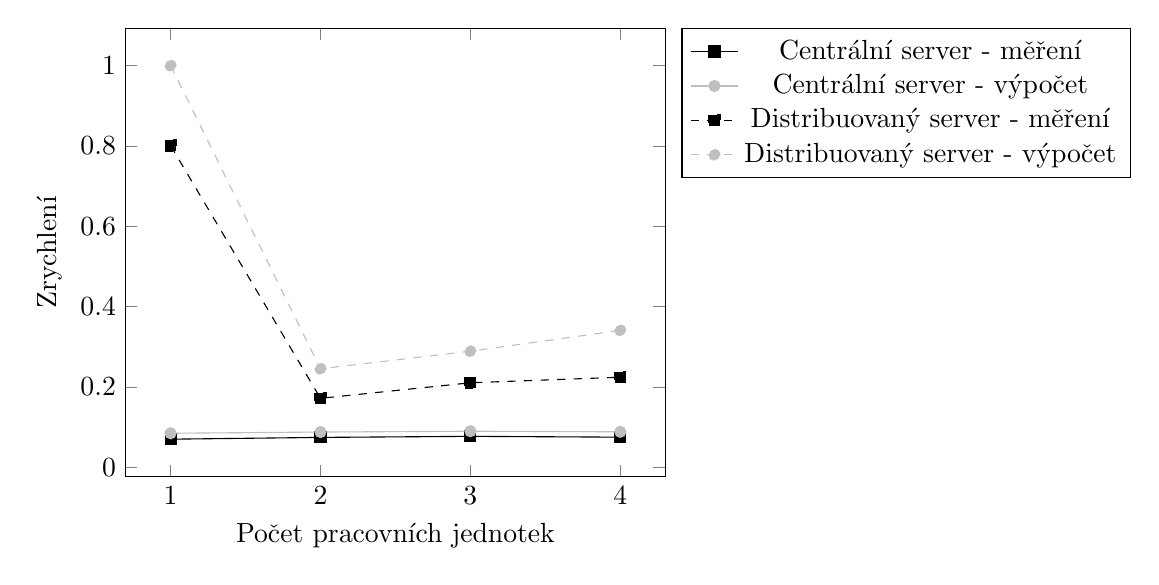
\begin{tikzpicture}
\begin{axis}[domain=1:4,xtick={1,2,3,4},xlabel={Počet pracovních jednotek},ylabel={Zrychlení},legend pos=outer north east]
\addplot[color=black,mark=square*]coordinates{(1,0.0697683325)(2,0.0742096687)(3,0.0768732879)(4,0.0748125092)};
\addplot[color=lightgray,mark=*]coordinates{(1,0.0845006079)(2,0.0875797841)(3,0.0895867948)(4,0.0882144472)};
\addplot[color=black,mark=square*,dashed]coordinates{(1,0.8008191205)(2,0.171497577)(3,0.210260728)(4,0.2240734765)};
\addplot[color=lightgray,mark=*,dashed]coordinates{(1,1)(2,0.2450480659)(3,0.2889043645)(4,0.3406430757)};
\legend{Centrální server - měření,Centrální server - výpočet,Distribuovaný server - měření,Distribuovaný server - výpočet}
\end{axis}
\end{tikzpicture}
\caption{Zrychlení trénování sítě VGG16E při použití synchronního trénování se spojením dávek.}
\label{gr:sync_join_vgg16e}
\end{figure}

Graf \ref{gr:sync_join_googlenet} ukazuje zrychlení trénování sítě GoogLeNet na jedné až osmi pracovních jednotkách.
Z~tohoto grafu vyplývá, že tato síť je vhodná pro distribuované trénování, protože ve všech případech dosahuje zrychlení vyššího než 1.
Pro centrální server bylo toto přesně předpovězeno pomocí výpočtu odhadu zrychlení.
Pro distribuovaný server byl odhad méně přesný, ale správně říkal, jak se zrychlení zachová se zvyšujícím se počtem pracovních jednotek.
Tyto odhady správně určily, že nejlepším způsobem jak trénovat síť GoogLeNet je použití distribuovaného serveru a osmi pracovních jednotek.

\begin{figure}
\centering
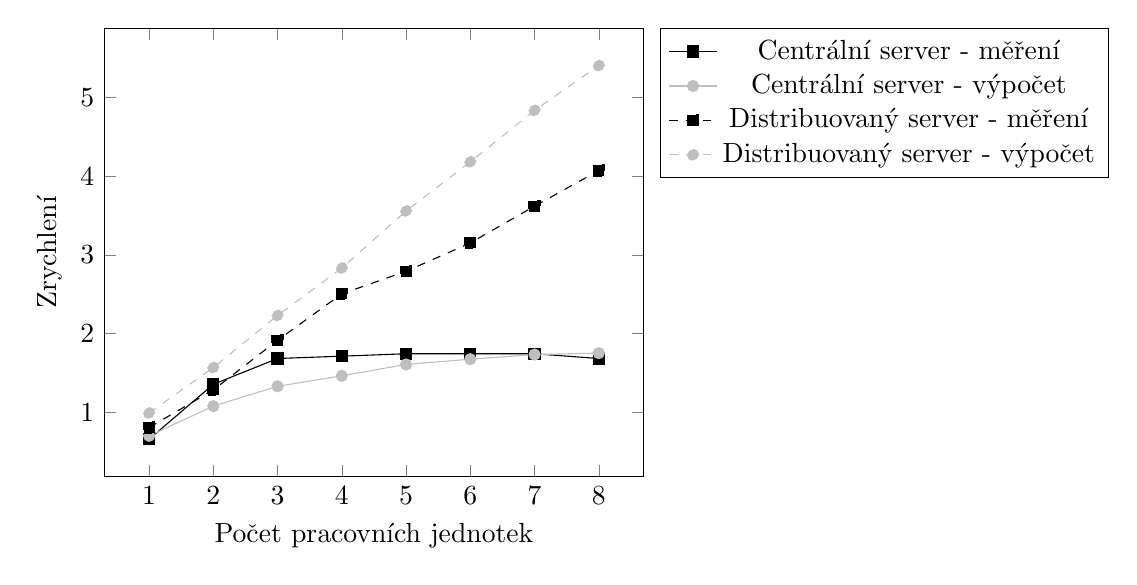
\begin{tikzpicture}
\begin{axis}[domain=1:8,xtick={1,2,3,4,5,6,7,8},xlabel={Počet pracovních jednotek},ylabel={Zrychlení},legend pos=outer north east]
\addplot[color=black,mark=square*]coordinates{(1,0.6601502887)(2,1.3569755935)(3,1.6845214264)(4,1.7140744339)(5,1.744682906)(6,1.744682906)(7,1.744682906)(8,1.6845214264)};
\addplot[color=lightgray,mark=*]coordinates{(1,0.7027592832)(2,1.0797030714)(3,1.3314030678)(4,1.4649503391)(5,1.6090284145)(6,1.6759416177)(7,1.7347251018)(8,1.7528795351)};
\addplot[color=black,mark=square*,dashed]coordinates{(1,0.8074565515)(2,1.2855558254)(3,1.9157302497)(4,2.5051857111)(5,2.7914926495)(6,3.1516852495)(7,3.6186015827)(8,4.0709267806)};
\addplot[color=lightgray,mark=*,dashed]coordinates{(1,0.992248062)(2,1.569093763)(3,2.2307898125)(4,2.8329983603)(5,3.5570531207)(6,4.1814025589)(7,4.83492834)(8,5.4032627024)};
\legend{Centrální server - měření,Centrální server - výpočet,Distribuovaný server - měření,Distribuovaný server - výpočet}
\end{axis}
\end{tikzpicture}
\caption{Zrychlení trénování sítě GoogLeNet při použití synchronního trénování se spojením dávek.}
\label{gr:sync_join_googlenet}
\end{figure}

Graf \ref{gr:sync_join_squeezenet} zobrazuje zrychlení trénování sítě SqueezeNet na jedné až osmi pracovních jednotkách.
Tento graf říká, že tato síť je velmi vhodná pro distribuované trénování, protože ve všech případech dosahuje zrychlení vyššího než 1.
Pro centrální server bylo toto přesně předpovězeno pomocí výpočtu odhadu zrychlení.
Pro distribuovaný server byl odhad méně přesný, ale správně říkal, jak se zrychlení zachová se zvyšujícím se počtem pracovních jednotek.
Tyto odhady správně určily, že nejlepším způsobem jak trénovat síť SqueezeNet je použití osmi pracovních jednotek.
Na typu použitého serveru nezáleží.
To je způsobeno velmi malým počtem vah této sítě.

\begin{figure}
\centering
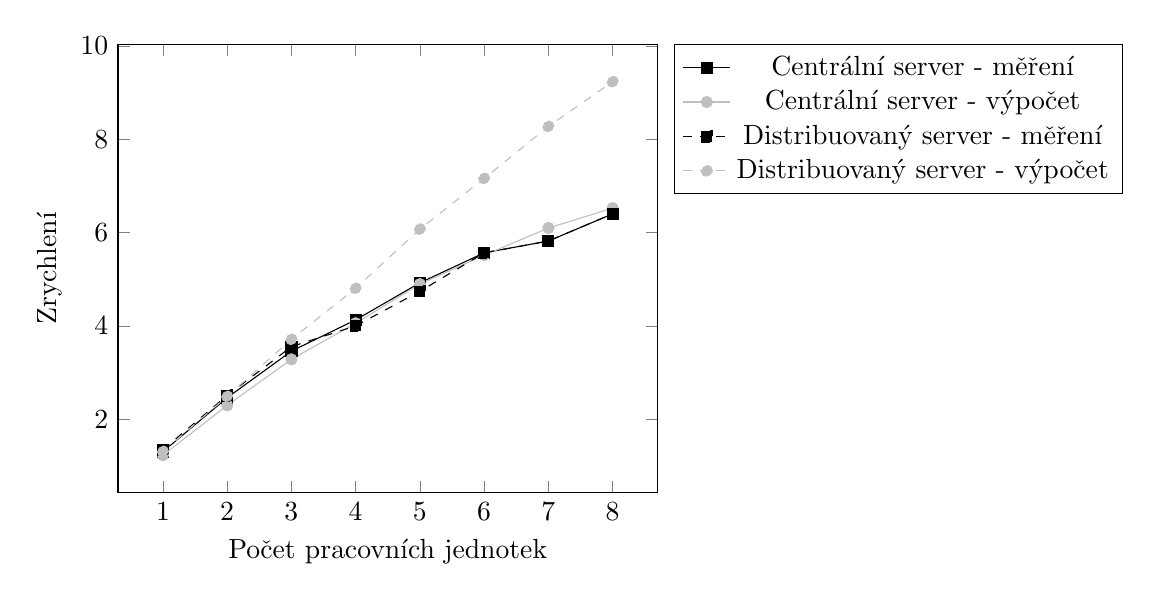
\begin{tikzpicture}
\begin{axis}[domain=1:8,xtick={1,2,3,4,5,6,7,8},xlabel={Počet pracovních jednotek},ylabel={Zrychlení},legend pos=outer north east]
\addplot[color=black,mark=square*]coordinates{(1,1.306122449)(2,2.4615384615)(3,3.4594594595)(4,4.1290322581)(5,4.9230769231)(6,5.5652173913)(7,5.8181818182)(8,6.4)};
\addplot[color=lightgray,mark=*]coordinates{(1,1.2291076898)(2,2.2981199353)(3,3.2838351138)(4,4.0569683372)(5,4.8952877237)(6,5.5134372866)(7,6.0974104024)(8,6.5219881601)};
\addplot[color=black,mark=square*,dashed]coordinates{(1,1.3473684211)(2,2.5098039216)(3,3.5555555556)(4,4)(5,4.7407407407)(6,5.5652173913)(7,5.8181818182)(8,6.4)};
\addplot[color=lightgray,mark=*,dashed]coordinates{(1,1.3095612077)(2,2.490303696)(3,3.7126663393)(4,4.8046936965)(5,6.0733903008)(6,7.1581776491)(7,8.272391696)(8,9.2322273034)};
\legend{Centrální server - měření,Centrální server - výpočet,Distribuovaný server - měření,Distribuovaný server - výpočet}
\end{axis}
\end{tikzpicture}
\caption{Zrychlení trénování sítě SqueezeNet při použití synchronního trénování se spojením dávek.}
\label{gr:sync_join_squeezenet}
\end{figure}

Zrychlení trénování sítě Resnet34 na jedné až osmi pracovních jednotkách zobrazuje graf \ref{gr:sync_join_resnet34}.
Z~tohoto grafu vyplývá, že síť Resnet34 je vhodná pro tento způsob distribuovaného trénování, protože ve všech případech dosahuje zrychlení vyššího než 1.
Pro centrální server bylo toto přesně předpovězeno pomocí výpočtu odhadu zrychlení.
Odhad zrychlení pro distribuovaný server byl méně přesný, ale správně předpověděl, jak se zachová při zvýšení počtu pracovních jednotek.
Tyto odhady správně určily, že nejlepším způsobem jak trénovat síť Resnet34 je použití osmi pracovních jednotek a distribuovaného serveru.

\begin{figure}
\centering
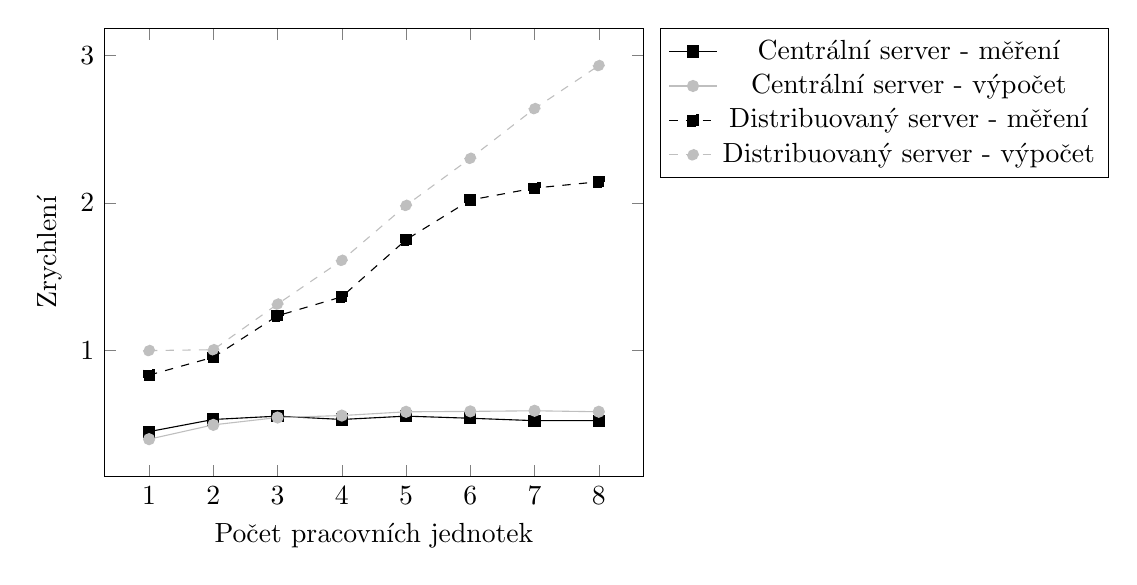
\begin{tikzpicture}
\begin{axis}[domain=1:8,xtick={1,2,3,4,5,6,7,8},xlabel={Počet pracovních jednotek},ylabel={Zrychlení},legend pos=outer north east]
\addplot[color=black,mark=square*]coordinates{(1,0.4508741315)(2,0.5332673737)(3,0.5558395377)(4,0.5332673737)(5,0.5558395377)(6,0.5415137764)(7,0.5252683631)(8,0.5252683631)};
\addplot[color=lightgray,mark=*]coordinates{(1,0.3997081134)(2,0.4966705391)(3,0.5464628319)(4,0.5597317406)(5,0.5852335211)(6,0.5880164777)(7,0.5921446289)(8,0.5855157104)};
\addplot[color=black,mark=square*,dashed]coordinates{(1,0.8337593066)(2,0.9550333875)(3,1.2359255603)(4,1.3643334108)(5,1.7508945438)(6,2.0202629352)(7,2.1010734526)(8,2.1439525026)};
\addplot[color=lightgray,mark=*,dashed]coordinates{(1,1)(2,1.0058906208)(3,1.3149228513)(4,1.6113233322)(5,1.9835271161)(6,2.3025694526)(7,2.6394072908)(8,2.9309359055)};
\legend{Centrální server - měření,Centrální server - výpočet,Distribuovaný server - měření,Distribuovaný server - výpočet}
\end{axis}
\end{tikzpicture}
\caption{Zrychlení trénování sítě Resnet34 při použití synchronního trénování se spojením dávek.}
\label{gr:sync_join_resnet34}
\end{figure}

\section{Synchronní trénování s~rozdělením dávek}
\label{sec:res_sync_split}

Tento způsob trénování jsem testoval na všech neuronových sítí kromě sítě VGG16E.
Na grafu \ref{gr:sync_split_googlenet} je zakreslena závislost zrychlení trénování sítě GoogLeNet na počtu pracovních jednotek.
Síť GoogLeNet je není vhodná pro trénování tímto způsobem, pokud je použit centrální server.
Při použití distribuovaného serveru je výhodnost tohoto způsobu trénování vyšší.
Přesnost odhadu pro centrální server je poměrně velká.
Pro distribuovaný server je odhad velmi nepřesný a dokonce říká, že se trénování zrychlí, přestože měření tvrdí opak.
Nejlepším způsobem jak trénovat 

\begin{figure}
\centering
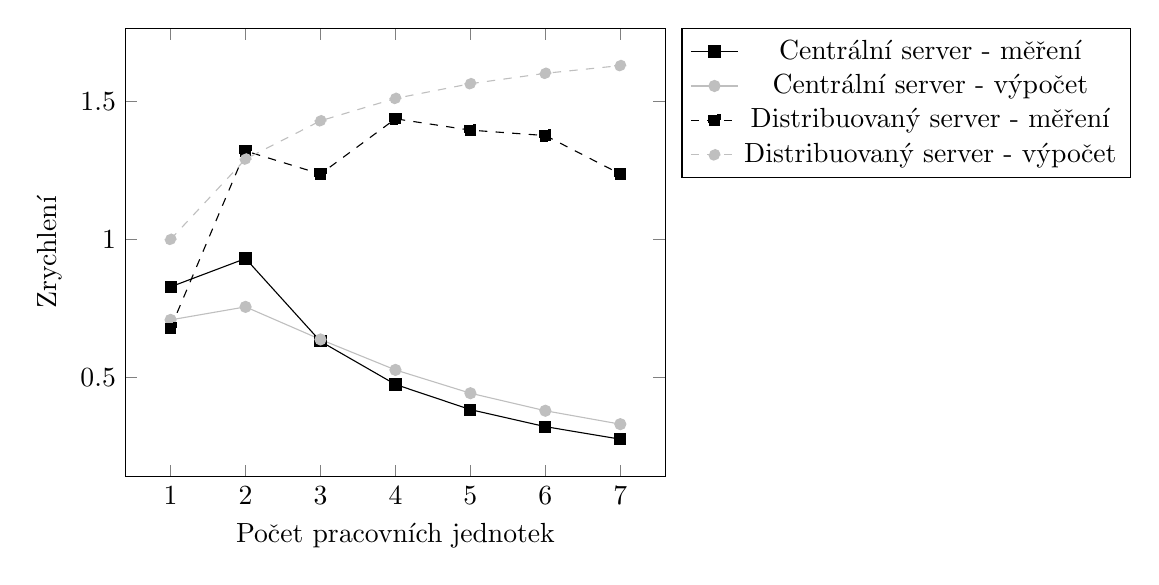
\begin{tikzpicture}
\begin{axis}[domain=1:7,xtick={1,2,3,4,5,6,7},xlabel={Počet pracovních jednotek},ylabel={Zrychlení},legend pos=outer north east]
\addplot[color=black,mark=square*]coordinates{(1,0.8279851079)(2,0.9304975498)(3,0.6303370499)(4,0.4742827317)(5,0.3831460499)(6,0.3213889564)(7,0.275995036)};
\addplot[color=lightgray,mark=*]coordinates{(1,0.7082495901)(2,0.7553650186)(3,0.6372965447)(4,0.5269463139)(5,0.4425448133)(6,0.3790382073)(7,0.3304279278)};
\addplot[color=black,mark=square*,dashed]coordinates{(1,0.6784877968)(2,1.3203005775)(3,1.2367372498)(4,1.4367976873)(5,1.3957463248)(6,1.3760879258)(7,1.2367372498)};
\addplot[color=lightgray,mark=*,dashed]coordinates{(1,1)(2,1.2909537514)(3,1.4296032252)(4,1.5107300372)(5,1.5639815268)(6,1.6016183246)(7,1.6296301928)};
\legend{Centrální server - měření,Centrální server - výpočet,Distribuovaný server - měření,Distribuovaný server - výpočet}
\end{axis}
\end{tikzpicture}
\caption{Zrychlení trénování sítě GoogLeNet při použití synchronního trénování s~rozdělením dávek.}
\label{gr:sync_split_googlenet}
\end{figure}

Graf \ref{gr:sync_split_squeezenet} ilustruje závislost zrychlení trénování sítě SqueezeNet na počtu pracovních jednotek.
Síť SqueezeNet je velmi vhodná pro trénování tímto způsobem pomocí obou typů serveru.
Při použití distribuovaného serveru je výhodnost tohoto způsobu trénování vyšší.
Pro oba typy serverů je odhad přesný a dokonce správně určuje, že při použití centrálního serveru je nejrychlejší výpočet na čtyřech pracovních jednotkách.
Nejlepším způsobem jak trénovat je použití distribuovaného serveru a osmi pracovních jednotek.

\begin{figure}
\centering
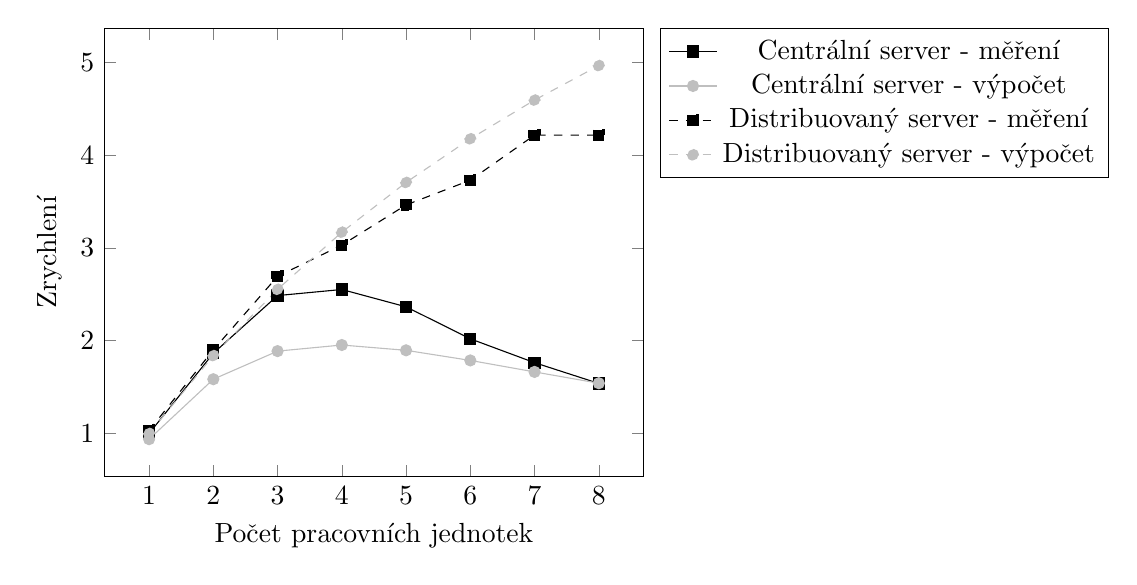
\begin{tikzpicture}
\begin{axis}[domain=1:7,xtick={1,2,3,4,5,6,7,8},xlabel={Počet pracovních jednotek},ylabel={Zrychlení},legend pos=outer north east]
\addplot[color=black,mark=square*]coordinates{(1,0.9998450318)(2,1.8650955401)(3,2.4867940535)(4,2.5522360022)(5,2.3654870265)(6,2.0205201684)(7,1.7633630561)(8,1.5394439379)};
\addplot[color=lightgray,mark=*]coordinates{(1,0.9385645226)(2,1.585002829)(3,1.8878472111)(4,1.9537836357)(5,1.8965102752)(6,1.7876047803)(7,1.663740994)(8,1.5416520428)};
\addplot[color=black,mark=square*,dashed]coordinates{(1,1.0317549796)(2,1.9016660409)(3,2.6940268913)(4,3.0307802527)(5,3.4637488602)(6,3.7301910802)(7,4.2167377428)(8,4.2167377428)};
\addplot[color=lightgray,mark=*,dashed]coordinates{(1,1)(2,1.839459684)(3,2.5541662015)(4,3.170005658)(5,3.7061656929)(6,4.1771705061)(7,4.5942164803)(8,4.9660736412)};
\legend{Centrální server - měření,Centrální server - výpočet,Distribuovaný server - měření,Distribuovaný server - výpočet}
\end{axis}
\end{tikzpicture}
\caption{Zrychlení trénování sítě SqueezeNet při použití synchronního trénování s~rozdělením dávek.}
\label{gr:sync_split_squeezenet}
\end{figure}

Na grafu \ref{gr:sync_split_resnet34} je zanesena závislost zrychlení trénování sítě Resnet34 na počtu pracovních jednotek.
Síť Resnet34 není vhodná pro trénování tímto způsobem pomocí obou typů serveru, protože zrychlení je vždy menší než 1.
Při použití distribuovaného serveru je zrychlení tohoto způsobu trénování vyšší, ale je stále menší než 1.
Pro centrální server je odhad velmi přesný.
Pro distribuovaný server je odhad méně přesný, ale stále správně předpovídá, jak se velikost zrychlení zachová při zvyšujícím se počtu pracovních jednotek.
Nejlepším způsobem jak trénovat je sekvenční trénování na jedné pracovní jednotce.

\begin{figure}
\centering
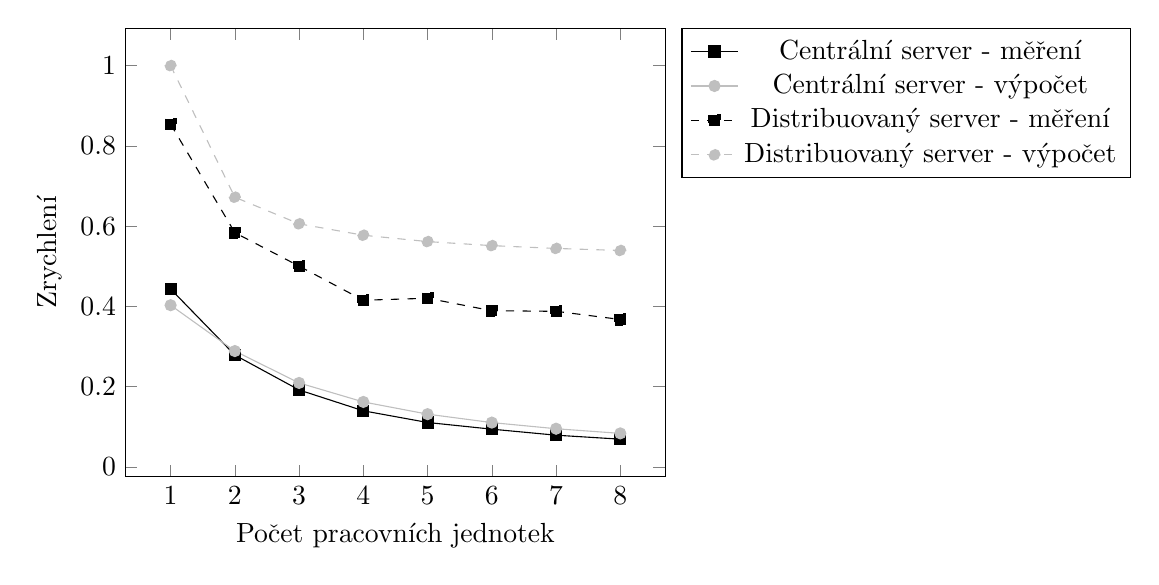
\begin{tikzpicture}
\begin{axis}[domain=1:7,xtick={1,2,3,4,5,6,7,8},xlabel={Počet pracovních jednotek},ylabel={Zrychlení},legend pos=outer north east]
\addplot[color=black,mark=square*]coordinates{(1,0.4432644415)(2,0.2786569566)(3,0.1917037822)(4,0.1396990328)(5,0.1105828133)(6,0.0939657179)(7,0.0789283791)(8,0.069023438)};
\addplot[color=lightgray,mark=*]coordinates{(1,0.402830833)(2,0.2886116788)(3,0.2091775297)(4,0.161819459)(5,0.1313687896)(6,0.1103599714)(7,0.0950581318)(8,0.0834414386)};
\addplot[color=black,mark=square*,dashed]coordinates{(1,0.8540948994)(2,0.5836315146)(3,0.5002555839)(4,0.4152319076)(5,0.4202146905)(6,0.3890876764)(7,0.3876519285)(8,0.3673205337)};
\addplot[color=lightgray,mark=*,dashed]coordinates{(1,1)(2,0.6719130755)(3,0.6056750537)(4,0.5772233575)(5,0.5614002305)(6,0.5513247756)(7,0.544346637)(8,0.5392278664)};
\legend{Centrální server - měření,Centrální server - výpočet,Distribuovaný server - měření,Distribuovaný server - výpočet}
\end{axis}
\end{tikzpicture}
\caption{Zrychlení trénování sítě Resnet34 při použití synchronního trénování s~rozdělením dávek.}
\label{gr:sync_split_resnet34}
\end{figure}

\section{Asynchronní trénování}
\label{sec:res_async}

Asynchronní trénování jsem provedl na všech neuronových sítích popsaných v~sekcích \ref{sec:vgg16e} až \ref{sec:resnet34}.
Na grafu \ref{gr:async_vgg16e} je zrychlení trénování sítě VGG16E tímto způsobem na jedné až čtyřech pracovních jednotkách.
Z~tohoto grafu vyplývá, že tato síť není vhodná pro distribuované trénování, protože ve všech případech dosahuje zrychlení nižšího než 1.
Pro centrální server bylo toto přesně předpovězeno pomocí výpočtu odhadu zrychlení.
Pro distribuovaný server byl odhad méně přesný.
Tento odhad ale správně říká, že nejlepším způsobem jak trénovat síť VGG16E je použití jedné pracovní jednotky a sekvenčního trénování.

\begin{figure}
\centering
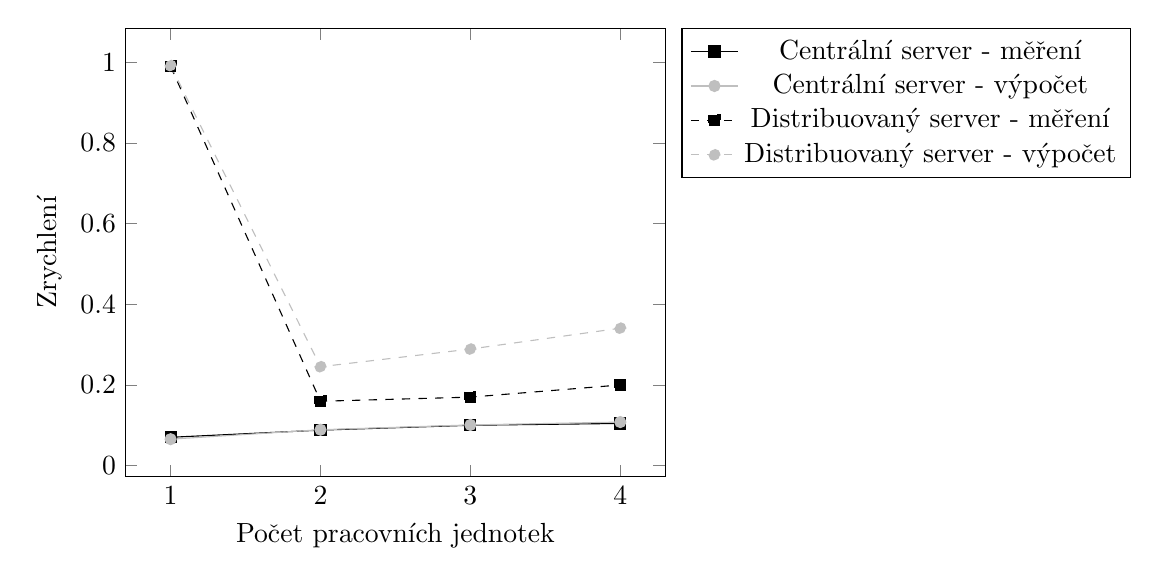
\begin{tikzpicture}
\begin{axis}[domain=1:4,xtick={1,2,3,4},xlabel={Počet pracovních jednotek},ylabel={Zrychlení},legend pos=outer north east]
\addplot[color=black,mark=square*]coordinates{(1,0.0699272581)(2,0.0877087608)(3,0.0997770302)(4,0.1042969409)};
\addplot[color=lightgray,mark=*]coordinates{(1,0.0652599741)(2,0.0887274335)(3,0.100622154)(4,0.1076889262)};
\addplot[color=black,mark=square*,dashed]coordinates{(1,0.9902602028)(2,0.159332524)(3,0.1696025762)(4,0.1997704964)};
\addplot[color=lightgray,mark=*,dashed]coordinates{(1,0.992248062)(2,0.2450480659)(3,0.2889043645)(4,0.3406430757)};
\legend{Centrální server - měření,Centrální server - výpočet,Distribuovaný server - měření,Distribuovaný server - výpočet}
\end{axis}
\end{tikzpicture}
\caption{Zrychlení trénování sítě VGG16E při použití asynchronního trénování.}
\label{gr:async_vgg16e}
\end{figure}

Graf \ref{gr:async_googlenet} ukazuje zrychlení trénování sítě GoogLeNet na jedné až osmi pracovních jednotkách.
Z~tohoto grafu vyplývá, že tato síť je vhodná pro distribuované trénování, protože ve všech případech dosahuje zrychlení vyššího než 1.
Pro oba typy serverů byl odhad méně přesný, ale správně říkal, jak se zrychlení zachová se zvyšujícím se počtem pracovních jednotek.
Tyto odhady správně určily, že nejlepším způsobem jak asynchronně trénovat síť GoogLeNet je použití distribuovaného serveru a osmi pracovních jednotek.

\begin{figure}
\centering
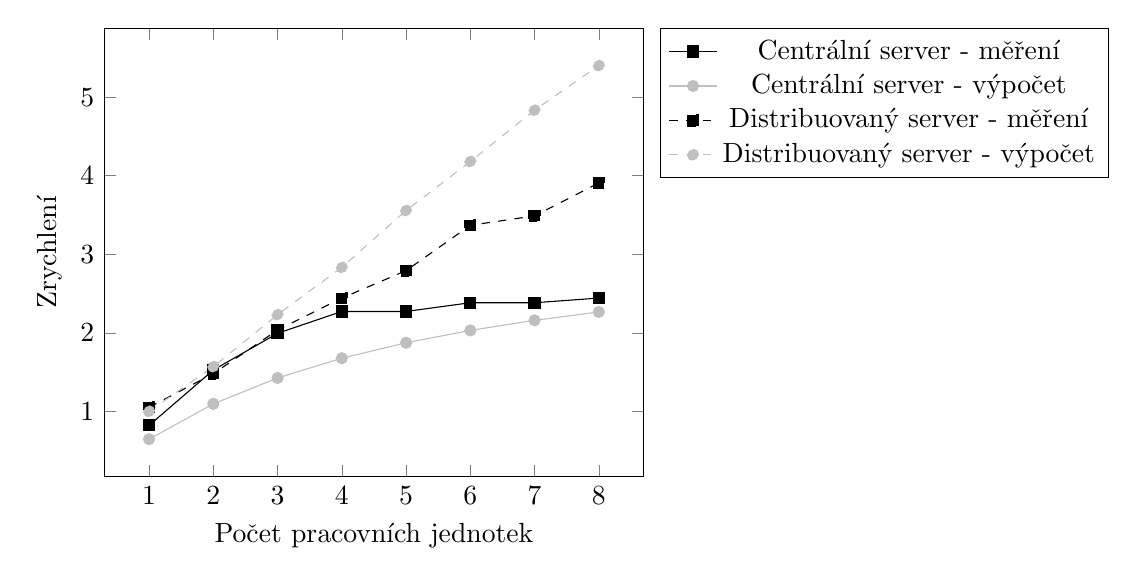
\begin{tikzpicture}
\begin{axis}[domain=1:8,xtick={1,2,3,4,5,6,7,8},xlabel={Počet pracovních jednotek},ylabel={Zrychlení},legend pos=outer north east]
\addplot[color=black,mark=square*]coordinates{(1,0.8210272499)(2,1.5265975427)(3,1.9939233211)(4,2.2721451799)(5,2.2721451799)(6,2.3829815301)(7,2.3829815301)(8,2.4425560683)};
\addplot[color=lightgray,mark=*]coordinates{(1,0.6454768757)(2,1.0952850079)(3,1.4252317811)(4,1.6764611776)(5,1.8732335621)(6,2.0307800061)(7,2.159145208)(8,2.2652216931)};
\addplot[color=black,mark=square*,dashed]coordinates{(1,1.0505617498)(2,1.4803370111)(3,2.0354633903)(4,2.4425560683)(5,2.7914926495)(6,3.3690428529)(7,3.4893658119)(8,3.9080897094)};
\addplot[color=lightgray,mark=*,dashed]coordinates{(1,1)(2,1.569093763)(3,2.2307898125)(4,2.8329983603)(5,3.5570531207)(6,4.1814025589)(7,4.83492834)(8,5.4032627024)};
\legend{Centrální server - měření,Centrální server - výpočet,Distribuovaný server - měření,Distribuovaný server - výpočet}
\end{axis}
\end{tikzpicture}
\caption{Zrychlení trénování sítě GoogLeNet při použití asynchronního trénování.}
\label{gr:async_googlenet}
\end{figure}

Graf \ref{gr:async_squeezenet} zobrazuje zrychlení trénování sítě SqueezeNet na jedné až osmi pracovních jednotkách.
Tento graf říká, že tato síť je velmi vhodná pro distribuované trénování, protože ve všech případech dosahuje zrychlení vyššího než 1.
Pro centrální server bylo toto přesně předpovězeno pomocí výpočtu odhadu zrychlení.
Pro distribuovaný server byl odhad méně přesný, ale správně říkal, jak se zrychlení zachová se zvyšujícím se počtem pracovních jednotek.
Tyto odhady správně určily, že nejlepším způsobem jak asynchronně trénovat síť SqueezeNet je použití osmi pracovních jednotek.
Na typu použitého serveru nezáleží.

\begin{figure}
\centering
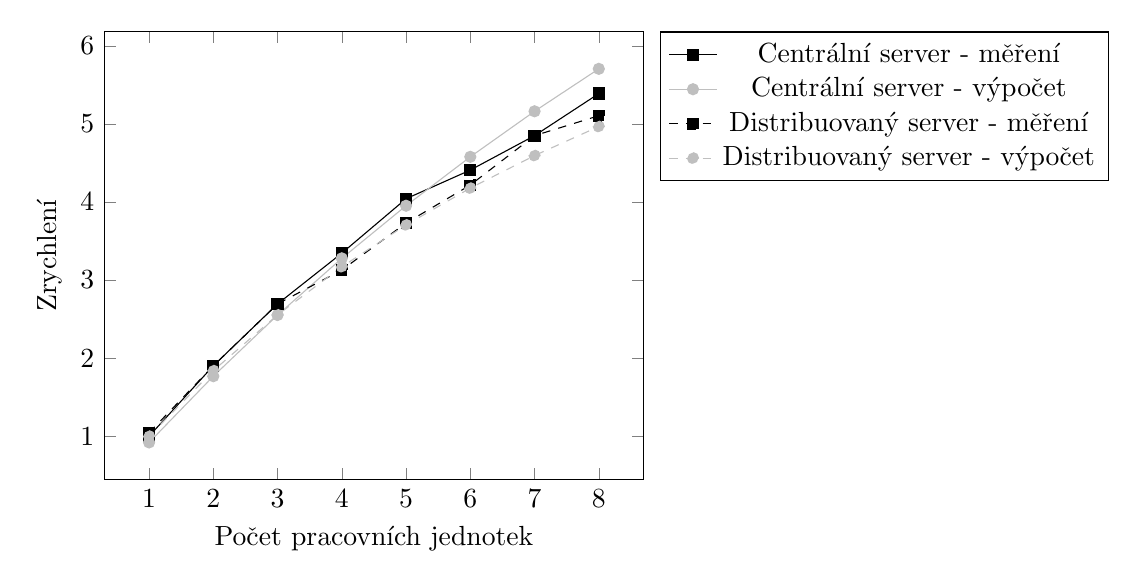
\begin{tikzpicture}
\begin{axis}[domain=1:8,xtick={1,2,3,4,5,6,7,8},xlabel={Počet pracovních jednotek},ylabel={Zrychlení},legend pos=outer north east]
\addplot[color=black,mark=square*]coordinates{(1,0.9998450318)(2,1.9016660409)(3,2.6940268913)(4,3.3443092443)(5,4.0410403369)(6,4.4084076402)(7,4.8492484043)(8,5.3880537825)};
\addplot[color=lightgray,mark=*]coordinates{(1,0.919729842)(2,1.7679485785)(3,2.5519440474)(4,3.2780570224)(5,3.9518300004)(6,4.5781287985)(7,5.1612425858)(8,5.7049666843)};
\addplot[color=black,mark=square*,dashed]coordinates{(1,1.0428491192)(2,1.9016660409)(3,2.6940268913)(4,3.1285473576)(5,3.7301910802)(6,4.2167377428)(7,4.8492484043)(8,5.1044720045)};
\addplot[color=lightgray,mark=*,dashed]coordinates{(1,1)(2,1.839459684)(3,2.5541662015)(4,3.170005658)(5,3.7061656929)(6,4.1771705061)(7,4.5942164803)(8,4.9660736412)};
\legend{Centrální server - měření,Centrální server - výpočet,Distribuovaný server - měření,Distribuovaný server - výpočet}
\end{axis}
\end{tikzpicture}
\caption{Zrychlení trénování sítě SqueezeNet při použití asynchronního trénování.}
\label{gr:async_squeezenet}
\end{figure}

Zrychlení trénování sítě Resnet34 na jedné až osmi pracovních jednotkách zobrazuje graf \ref{gr:async_resnet34}.
Z~tohoto grafu vyplývá, že síť Resnet34 je vhodná pro tento způsob distribuovaného trénování, pouze pokud se použije distribuovaný server.
Pro trénování pomocí centrálního serveru tato síť není vhodná, protože zrychlení trénování je nižší než 1.
To bylo přesně předpovězeno pomocí výpočtu.
Odhad zrychlení pro distribuovaný server je méně přesný, ale správně předpověděl, jak se zachová při zvýšení počtu pracovních jednotek.
Tyto odhady správně určily, že nejlepším způsobem jak asynchronně trénovat síť Resnet34 je použití osmi pracovních jednotek a distribuovaného serveru.

\begin{figure}
\centering
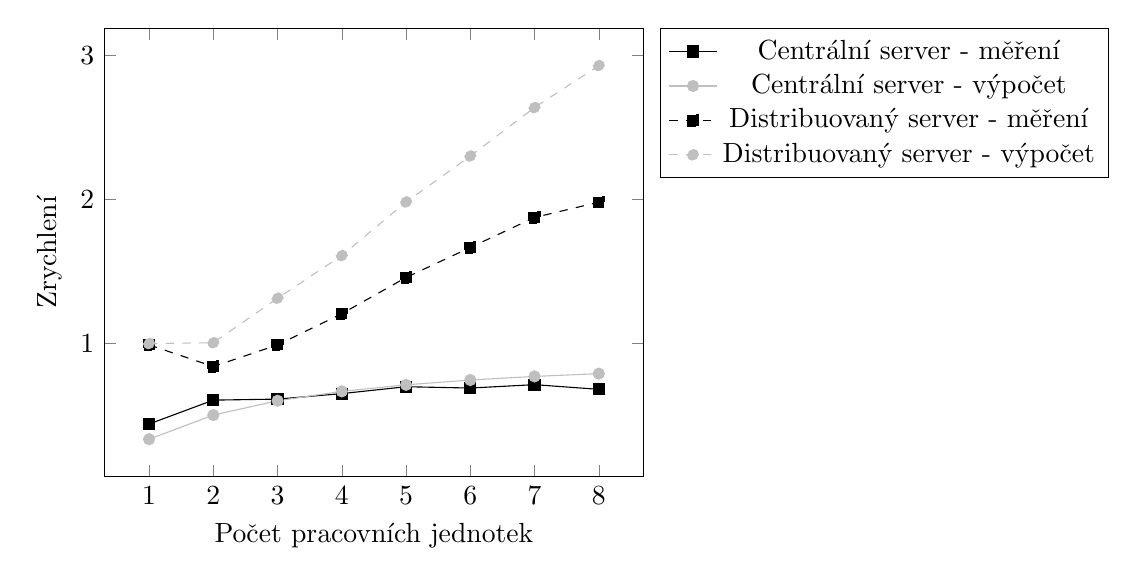
\begin{tikzpicture}
\begin{axis}[domain=1:8,xtick={1,2,3,4,5,6,7,8},xlabel={Počet pracovních jednotek},ylabel={Zrychlení},legend pos=outer north east]
\addplot[color=black,mark=square*]coordinates{(1,0.4414019858)(2,0.6072466626)(3,0.6143489627)(4,0.6525072834)(5,0.7003578175)(6,0.6911425831)(7,0.7146508342)(8,0.6821667054)};
\addplot[color=lightgray,mark=*]coordinates{(1,0.3359565378)(2,0.503450619)(3,0.602855849)(4,0.6680289176)(5,0.7135786103)(6,0.7468418646)(7,0.7719075949)(8,0.7912348817)};
\addplot[color=black,mark=square*,dashed]coordinates{(1,0.9910723833)(2,0.840429381)(3,0.9910723833)(4,1.2075134785)(5,1.4590787865)(6,1.6675186131)(7,1.8759584398)(8,1.9821447666)};
\addplot[color=lightgray,mark=*,dashed]coordinates{(1,1)(2,1.0058906208)(3,1.3149228513)(4,1.6113233322)(5,1.9835271161)(6,2.3025694526)(7,2.6394072908)(8,2.9309359055)};
\legend{Centrální server - měření,Centrální server - výpočet,Distribuovaný server - měření,Distribuovaný server - výpočet}
\end{axis}
\end{tikzpicture}
\caption{Zrychlení trénování sítě Resnet34 při použití asynchronního trénování.}
\label{gr:async_resnet34}
\end{figure}

%===============================================================================

\chapter{Diskuze}
\label{chap:disc}

V~této kapitole shrnu výsledky, které jsem prezentoval v~předchozí kapitole.
První polovinu této kapitoly zabírá zhodnocení výsledků experimentů.
Druhá polovina je věnována návrhu mechanizmu, který by měl zrychlit paralelní trénování pomocí optimalizace komunikace se serverem.

\section{Zhodnocení výsledků}
\label{sec:res_eval}

Při sekvenčním trénování jsem naměřil délky výpočtu jedné dávky a přenosu vah od serveru k~pracovní jednotce.
Délky výpočtu gradientů všech čtyř sítí jsou si podobné, i když se sítě liší ve struktuře a počtu vah.
To považuji za velmi výhodné, protože délky přenosu tak budou mít hlavní vliv na celkovou délku trénování.
Délky přenosu vah sítí se výrazně liší v~závislosti na jejich počtu.
SqueezeNet je síť s~nejmenším počtem vah a délka přenosu byla nejkratší.
Délka přenosu vah sítě GoogLeNet je přibližně sedmkrát delší.
Váhy sítě Resnet34 se přenesou za 27krát delší dobu.
Pro síť VGG16E přenos vah trval 170krát déle než pro síť SqueezeNet.
Délky přenosu vah odpovídají počtu parametrů sítě.

Síť VGG16E je velmi nevhodná pro paralelní trénování, protože používá velké množství vah.
Jejich přenosy tak velmi výrazně zpomalovaly trénování sítě.
Výsledkem je to, že nejlepším způsobem jak trénovat tuto síť je sekvenční trénování na jedné pracovní jednotce.

Resnet34 také není vhodná pro paralelní trénování, protože používá velké množství vah.
Nejlepšího výsledku jsem dosáhl, když jsem Resnet34 synchronně trénoval na osmi pracovních jednotkách pomocí distribuovaného serveru.
V~tom případě bylo zrychlení 2,1.
To je velmi malé zrychlení na to, že jsem použil osm pracovních jednotek.

Síť GoogLeNet je vhodná pouze v~některých případech.
Při asynchronním trénování je dosaženo zrychlení 3,9 a při použití synchronního trénování s~rozdělením dávek zrychlení 4.
V~obou případech musí být použit distribuovaný server, jinak je zrychlení výrazně horší.

SqueezeNet je síť, která byla navržena, aby měla velmi malý počet vah.
To je velmi výhodné pro její paralelní trénování a projevuje se to velmi výrazným zrychlením při trénování na více výpočetních jednotkách.
Nejlepší výsledek je zrychlení 6,5, kterého bylo dosaženo při synchronním trénování se spojením dávek na osmi pracovních jednotkách pomocí distribuovaného serveru.

Ve většině případů bylo nejlepším způsobem trénování použití osmi výpočetních jednotek a distribuovaného serveru nebo sekvenční trénování na jedné jednotce.
Zajímavým případem je trénování sítě SqueezeNet při použití synchronního trénování s~rozdělením dávek pomocí centrálního serveru.
Toto trénování je popsané grafem \ref{gr:sync_split_squeezenet}.
V~tomto případě je trénování nejrychlejší při použití čtyř výpočetních jednotek.
Výpočet odhadů tento nezvyklý případ předpověděl.

Zrychlení při použití distribuovaného serveru bylo většinou větší než při použití centrálního serveru.
Jediným případem, kdy bylo přibližně stejně velké, je při asynchronním a synchronním trénování se spojením dávek sítě SqueezeNet.
To bylo způsobeno velmi malým počtem vah této sítě.
Kvůli tomu je vliv zrychlené komunikace na celkovou délku výpočtu velmi malý.
Ve všech ostatních případech použití distribuovaného serveru zvýšilo zrychlení trénování.
To je způsobeno velmi malým počtem vah této sítě.

Krajním případem bylo distribuované trénování na jedné pracovní jednotce.
Při použití centrálního serveru bylo trénování vždy pomalejší než sekvenční.
To je tím, že se vlastně jedná o~sekvenční trénování, které před a po každém výpočtu gradientů provádí přenos dat z~a na server.
Toto trénování bude vždy pomalejší než sekvenční trénování na jedné jednotce.
To se potvrdilo při výpočtu i při experimentování.
Při použití distribuovaného serveru bylo trénování mírně pomalejší než sekvenční.
To je způsobeno dodatečnými přenosy vah a gradientů v~rámci jedné jednotky, mezi serverovou a výpočetní částí jednotky.

\section{Návrh na další práci}
\label{sec:prop}

V~kapitole \ref{chap:est} jsem při trénování s~centrálním serverem popsal případ nejlepšího rozložení komunikace a výpočtů.
Tento případ využíval toho, že k~serveru přistupovala pouze jedna pracovní jednotka.
To způsobilo, že komunikace probíhala na nejvyšší možné rychlosti.
To je ideální případ, který málokdy nastane.
Existuje ale způsob jak zaručit, že tento případ nastane pokaždé, když se bude k~serveru přistupovat.
Je totiž možné zaručit exkluzivní přístup k~serveru pomocí semaforu.

Navrhuji tedy vytvoření systému, který bude řídit přístup k~serveru.
Tento systém bude založen na semaforu definovaném Edsgerem W. Dijkstrou v~práci \cite{Dijkstra2002}.
Na serveru bude umístěn semafor s~frontou, který omezuje přenos dat se serverem pouze na jednu pracovní jednotku.
Ostatní jednotky musí čekat ve frontě, pokud chtějí přístup k~serveru.
Velmi krátké přenosy dat (ve srovnání s~přenosem vah a gradientů) tomuto semaforu nepodléhají pro snížení režie.
Pro server s~duplexním spojením mezi ním a pracovními jednotkami je potřeba vytvořit dva semafory: jeden pro přenos dat směrem na server a druhý pro přenos dat ze serveru.

Pokud se serverem komunikuje všech $N$ pracovních jednotek zároveň, pak je délka této komunikace $t_{par}=Nt_{comm}$.
Pokud pracovní jednotky přistupují k~serveru jedna po druhé, pak je délka přenosu dat vždy $t_{comm}$.
V~nejlepším případě je fronta semaforu volná, potom je délka komunikace \begin{equation}t_{sem}^{BEST}=0t_{comm}+t_{comm}=t_{comm}.\end{equation}
V~tomto případě nemusí jednotka čekat ve frontě a může okamžitě začít komunikovat.
V~nejhorším případě je ve frontě $N-1$ pracovních jednotek, potom je délka komunikace \begin{equation}t_{sem}^{WORST}=(N-1)t_{comm}+t_{comm}=Nt_{comm}=t_{par}.\end{equation}
To znamená, že jednotka musí čekat, než předchozích $N-1$ procesů dokončí své přenosy dat.
Pro reálnou délku komunikace omezenou semaforem musí platit \begin{equation}t_{sem} \in \langle t_{sem}^{BEST}, t_{sem}^{WORST}\rangle.\end{equation}
Z~toho vyplývá, že $t_{sem} \leq t_{par}$.

Tento mechanizmus je možné zkombinovat s distribuovaným serverem.

%===============================================================================

\chapter{Závěr}
\label{chap:conc}

Má práce se zabývá paralelním trénováním neuronových sítí.
Její hlavní částí je návrh vzorců, které je možné použít na odhad délky trénování sítě na základě délky trénování jedné dávky a doby přenosu vah ze serveru na pracovní jednotku.
Z~délky trénování je možné vypočítat zrychlení trénování na daném počtu pracovních jednotek.
Pro ověření přesnosti těchto vzorců jsem provedl experimenty, které testovali přesnost odhadu zrychlení trénování čtyř neuronových sítí třemi různými způsoby pomocí dvou typů serveru s~parametry.
Tyto experimenty ukázali, že výpočty navržené v~této práci je možné použít k~odhadu doby trénování a zrychlení.
V~každém případě trénování výpočty určily ideální počet výpočetních jednotek a typ serveru.
Pro implementaci trénování jsem použil knihovnu Tensorflow. 

Pro sítě s~velmi velkým počtem parametrů jako je VGG16E je nejvhodnější sekvenční trénování na jedné pracovní jednotce, protože doba strávená přenosem vah a gradientů je velmi velmi vysoká a zabraňuje zrychlení výpočtu.
Ve všech případech paralelního trénování této sítě bylo zrychlení menší jak 1, to bylo předpovězeno pomocí výpočtu.
Přestože síť Resnet34 má menší počet vah ve srovnání s~dříve uvedenou sítí, paralelní trénování této sítě nebylo výhodné.
Použití distribuovaného serveru bylo nutné pro dosažení zrychlení většího než 1.
Síť GoogLeNet má malý počet vah ve srovnání s~dříve uvedenými sítěmi, a proto paralelní trénování této sítě bylo výhodnější.
Přestože má tato síť méně vah než předchozí sítě, je stále použití distribuovaného serveru vhodné pro dosažení vyššího zrychlení.
Sítě s~velmi malým počtem vah jako je SqueezeNet se trénují velmi dobře na více paralelních jednotkách.
Doba strávené přenosem vah nebo gradientů je velmi malá ve srovnání s~dobou výpočtu gradientů jedné dávky.
Při trénování sítě SqueezeNet na osmi výpočetních jednotkách jsem dosáhl zrychlení 6,5.
Ve všech případech dokázaly moje odhady určit, jak se bude měnit velikost zrychlení trénování sítě při trénování na více výpočetních jednotkách.

Druhou nejdůležitější částí práce je návrh distribuovaného serveru.
Cílem tohoto serveru zkrácení doby komunikace a tudíž i trénování.
Toho je dosaženo zvýšením využití duplexního spojení mezi jednotkami, které provádějí trénování.
Distribuovaný server zvýšil zrychlení nebo dosáhl stejného zrychlení jako centrální server ve všech případech.
Použití distribuovaného serveru nikdy nezpůsobilo snížení zrychlení.

Dále jsem navrhl mechanizmus pro zefektivnění předávání vah a gradientů při trénování.
Cílem tohoto mechanizmu je zajistit co nejrychlejší přenos dat mezi jednotkami.
Toho by se mělo dosáhnout pomocí omezení počtu jednotek, které komunikují s~jednou jednotkou v~každém směru, pomocí semaforu.
Tento mechanizmus je možné zkombinovat s~distribuovaným serverem.

%===============================================================================
